%%%%%%%%%%%%%%%%%%%%%%%%%%%%%%%%%%%%%%%%%%%%%%%%%%%%%%%%%%%%%%%%%%%%%%%%%%%%
%                                                                          %
%              (C) Copyright 1995 The Board of Trustees of the             %
%                          University of Illinois                          %
%                           All Rights Reserved                            %
%								  	   %
%%%%%%%%%%%%%%%%%%%%%%%%%%%%%%%%%%%%%%%%%%%%%%%%%%%%%%%%%%%%%%%%%%%%%%%%%%%%

%%%%%%%%%%%%%%%%%%%%%%%%%%%%%%%%%%%%%%%%%%%%%%%%%%%%%%%%%%%%%%%%%%%%%%%%%%%%
% RCS INFORMATION:
%
%       $RCSfile: ug.tex,v $
%       $Author: jim $        $Locker:  $                $State: Exp $
%       $Revision: 1.8 $      $Date: 2002/02/20 22:26:04 $
%
%%%%%%%%%%%%%%%%%%%%%%%%%%%%%%%%%%%%%%%%%%%%%%%%%%%%%%%%%%%%%%%%%%%%%%%%%%%%
% DESCRIPTION:
%
%%%%%%%%%%%%%%%%%%%%%%%%%%%%%%%%%%%%%%%%%%%%%%%%%%%%%%%%%%%%%%%%%%%%%%%%%%%%
% REVISION HISTORY:
%
% $Log: ug.tex,v $
% Revision 1.8  2002/02/20 22:26:04  jim
% Added alchemical free energy docs "as is", fixed only to build.
%
% Revision 1.7  2002/02/13 16:40:30  jim
% Moved psfgen to separate directory tree based on Justin's version.
%
% Revision 1.6  2001/02/23 02:03:04  jim
% Added documentation on psfgen.
%
% Revision 1.5  1999/10/08 02:29:36  jim
% Now works with LaTeX 2e and can produce PDF files.
%
% Revision 1.4  1999/02/26 06:57:15  jim
% Changes to make latex2html work.
%
% Revision 1.3  1999/02/02 21:35:29  jim
% Added free energy documentation from David Hurwitz.
%
% Revision 1.2  1998/08/21 02:26:22  jim
% Added more docs, cleaned up a bit, switched figure system.
%
% Revision 1.1  1998/01/05 21:12:30  dhardy
% user guide, first draft
%
% Revision 1.4  1996/05/20 16:39:37  brunner
% Put all necessary bib entries into ug.bib, to remove duplicate entries.
%
% Revision 1.3  1996/05/15 19:21:07  jean
% ready (I hope) for 1.4 beta release
%
% Revision 1.2  1996/03/24 21:53:19  jean
% failed attempt to increase subsection depth (sigh)
%
% Revision 1.1  1995/06/19 16:08:14  nelson
% Initial revision
%
%%%%%%%%%%%%%%%%%%%%%%%%%%%%%%%%%%%%%%%%%%%%%%%%%%%%%%%%%%%%%%%%%%%%%%%%%%%%

\documentclass[11pt]{article}
\usepackage{graphicx}

% define margins, etc
\topmargin	0.1in
\oddsidemargin	0in
\evensidemargin	0in
\textheight	8.80in
\textwidth	6.50in
\marginparsep	0.25cm
\headheight	0in
\headsep	0in
%\footskip	0.5in
%\footheight	0in%

% define macros
%%%%%%%%%%%%%%%%%%%%%%%%%%%%%%%%%%%%%%%%%%%%%%%%%%%%%%%%%%%%%%%%%%%%%%%%%%%%
%                                                                          %
%              (C) Copyright 1995 The Board of Trustees of the             %
%                          University of Illinois                          %
%                           All Rights Reserved                            %
%								  	   %
%%%%%%%%%%%%%%%%%%%%%%%%%%%%%%%%%%%%%%%%%%%%%%%%%%%%%%%%%%%%%%%%%%%%%%%%%%%%

%
% generally useful macros
%
\newcommand{\REFAND} {\&}
\newcommand{\ETALNP}{\mbox{\it et al}}
\newcommand{\ETAL}{\mbox{\ETALNP{\it.}}}
\newcommand{\eqnref}[1] {\mbox{eq (\ref{#1})}}
\newcommand{\mycite}[2] {\cite{#2}}
%\newcommand{\mycite}[2] {}

\newcommand{\NAMD} {NAMD}
\newcommand{\NAMDDATE} {\today}
\newcommand{\NAMDAUTHORS} {M.~Bhandarkar, A.~Bhatele, E.~Bohm, R.~Brunner, F.~Buelens, C.~Chipot, A.~Dalke, S.~Dixit, G.~Fiorin, P.~Freddolino, P.~Grayson, J.~Gullingsrud, A.~Gursoy, D.~Hardy, C.~Harrison, J.~H\'enin, W.~Humphrey, D.~Hurwitz, N.~Krawetz, S.~Kumar, D.~Kunzman, C.~Lee, C.~Mei, M.~Nelson, J.~Phillips, O.~Sarood, A.~Shinozaki, G.~Zheng, F.~Zhu}

% The file namd_version.tex is automatically generated by the Makefile.

\newcommand{\NAMD} {NAMD}
\newcommand{\NAMDDATE} {\today}
\newcommand{\NAMDVER} {2.3b1}
\newcommand{\NAMDAUTHORS} {M.~Bhandarkar, R.~Brunner, A.~Dalke, J.~Gullingsrud, A.~Gursoy, W.~Humphrey, D.~Hurwitz, N.~Krawetz, M.~Nelson, J.~Phillips, A.~Shinozaki}



%
% macros for style conventions when describing the program.
%

% name of class or object in program
\newcommand{\OBJ}[1] {{\bf\tt#1}}

% function arguments
\newcommand{\FA}[2] {{\rm{\bf#1}\ {\it#2}}}

% global function name
\newcommand{\FN}[3] {{\rm\bf#1}\ {\tt #2(}#3{\tt)}}

% class member function name
\newcommand{\FNO}[4] {{\rm\bf#2}\ \OBJ{#1::}{\tt#3(}#4{\tt)}}

% list item, for optional components, parameters, etc.
\newcommand{\TTLISTITEM}[1] {\item {\tt #1} \\}
\newcommand{\RMLISTITEM}[1] {\item {\rm #1} \\}
\newcommand{\BOLDLISTITEM}[1] {\item {\bf #1} \\}
\newcommand{\EMLISTITEM}[1] {\item {\em #1} \\}
\newcommand{\LISTITEM}[1] {\RMLISTITEM{#1}}

%
% other generally useful macros
%

% Other program names, formatted nicely
\newcommand{\FEP} {FEP}
\newcommand{\VMD} {VMD}
\newcommand{\MDCOMM} {MDComm}
\newcommand{\MDSCOPE} {MDScope}
\newcommand{\CESB} {MDScope}
\newcommand{\ALLNAMES} {MDScope}
\newcommand{\SMALLMDSCOPE} {mdscope}
\newcommand{\SMALLCESB} {mdscope}
\newcommand{\SMALLALLNAMES} {mdscope}

% full name for MDScope, i.e., what it stands for
\newcommand{\MDSCOPENAME} {Molecular Dynamics computational environment}

% title of MDScope paper
\newcommand{\MDSCOPEPAPER} {MDScope: A Visual Computing Environment for
Structural Biology}

% default definitions for title and description
% \newcommand{\DOCTITLE} {Documentation Guides}
% \newcommand{\DOCDESC} {
%   This document includes the \NAMD\ Installation, Users, and
% Programmers Guides, which document how to obtain, install, use, and
% modify the molecular graphics program \NAMD.}


%%%%%%%%%%%%%%%%%%%%%%%%%%%%%%%%%%%%%%%%%%%%%%%%%%%%%%%%%%%%%%%%%%%%%%%%%%%%
%                                                                          %
%              (C) Copyright 1995 The Board of Trustees of the             %
%                          University of Illinois                          %
%                           All Rights Reserved                            %
%								  	   %
%%%%%%%%%%%%%%%%%%%%%%%%%%%%%%%%%%%%%%%%%%%%%%%%%%%%%%%%%%%%%%%%%%%%%%%%%%%%

\newcommand{\DOCTITLE} {User's Guide}
\newcommand{\DOCDESC} {%
The \NAMD\ {\em\DOCTITLE\/} describes how to run and use the 
various features of the molecular dynamics program \NAMD.  
This guide includes the capabilities of the program, how 
to use these capabilities, the necessary input files and 
formats, and how to run the program both on uniprocessor 
machines and in parallel.}
\newcommand{\PG}{\NAMD\ {\it Programmer's Guide\/}}
\newcommand{\UG}{\NAMD\ {\it User's Guide\/}}
\newcommand{\prettypar}{

\smallskip

}

%%%%%%%%%%%%%%%%%%%%%%%%%%%%%%%%%%%%%%%%%%%%%%%%%%%%%%%%%%
% GENERAL STUFF
%%%%%%%%%%%%%%%%%%%%%%%%%%%%%%%%%%%%%%%%%%%%%%%%%%%%%%%%%%

\newcommand{\eg}{{\it e.g.\/}}
\newcommand{\ie}{{\it i.e.\/}}

%%%%%%%%%%%%%%%%%%%%%%%%%%%%%%%%%%%%%%%%%%%%%%%%%%%%%%%%%%
% FORMULAE
%%%%%%%%%%%%%%%%%%%%%%%%%%%%%%%%%%%%%%%%%%%%%%%%%%%%%%%%%%

\newcommand{\gradx}{\mbox{\boldmath$\nabla_{\!\!x}\,$}}
\newcommand{\vx}{{\mbox{\boldmath{$x$}}}}
\newcommand{\bm}[1]{{\mbox{\boldmath{$#1$}}}}


\newcommand{\KEY}[1]{{\tt #1}}
\newcommand{\IKEY}[1]{{\tt #1\index{#1 psfgen command}}}
\newcommand{\OKEY}[1]{$[${\tt #1}$]$}
\newcommand{\ARG}[1]{$<${\em #1}$>$}
\newcommand{\OARG}[1]{$[${\em #1}$]$}
\newcommand{\ARGDEF}[2]{$<${\em #1}$>$: #2}
\newcommand{\KEYDEF}[2]{{\tt #1}: #2}
\newcommand{\COMMAND}[4]{%
  #1 \\ {\bf Purpose:} #2 \\ {\bf Arguments:} #3 \\ {\bf Context:} #4 }

\newcommand{\icommand}[1]{#1\index{#1 command}}

\newcommand{\NAMDCONF}[4]{%
%  \addcontentsline{toc}{subparagraph}{#1}%
  {\bf \tt #1 } $<$ #2 $>$ \index{#1 parameter} \\%
  {\bf Acceptable Values: } #3 \\%
  {\bf Description: } #4%
}

\newcommand{\NAMDCONFWDEF}[5]{%
%  \addcontentsline{toc}{subparagraph}{#1}%
  {\bf \tt #1 } $<$ #2 $>$ \index{#1 parameter} \\%
  {\bf Acceptable Values: } #3 \\%
  {\bf Default Value: } #4 \\%
  {\bf Description: } #5%
}

\newcommand{\NAMDCONFTAG}[4]{%
%  \addcontentsline{toc}{subparagraph}{#1}%
  {\bf \tt #1 } $<$ tag $>$ $<$ #2 $>$ \index{#1 parameter} \\%
  {\bf Acceptable Values: } #3 \\%
  {\bf Description: } #4%
}

\newcommand{\NAMDCONFTAGWDEF}[5]{%
%  \addcontentsline{toc}{subparagraph}{#1}%
  {\bf \tt #1 }  $<$ tag $>$ $<$ #2 $>$ \index{#1 parameter} \\%
  {\bf Acceptable Values: } #3 \\%
  {\bf Default Value: } #4 \\%
  {\bf Description: } #5%
}
\newcommand{\XNCOMP}[3]{%
  {\bf \NAMD\ Parameter: \tt #1 } \\%
  {\bf X-PLOR Parameter: \tt #2 } \\%
  #3%
}


\input{psfgen_macros}

\setcounter{secnumdepth}{3}
%% \setcounter{tocdepth}{5} %% very detailed table of contents
\setcounter{tocdepth}{4}

%
% the document itself
%

\begin{document}

% initial pages for the guide - title, TOC, etc.
%%%%%%%%%%%%%%%%%%%%%%%%%%%%%%%%%%%%%%%%%%%%%%%%%%%%%%%%%%%%%%%%%%%%%%%%%%%%
%                                                                          %
%              (C) Copyright 1995 The Board of Trustees of the             %
%                          University of Illinois                          %
%                           All Rights Reserved                            %
%								  	   %
%%%%%%%%%%%%%%%%%%%%%%%%%%%%%%%%%%%%%%%%%%%%%%%%%%%%%%%%%%%%%%%%%%%%%%%%%%%%

% title page

\thispagestyle{empty}

\vspace*{0.3in}

\begin{centering}
  \rule{6in}{0.04in}				\\	\vspace{0.25in}
  {\Huge \NAMD\ \DOCTITLE}			\\	\vspace{0.25in}
  {\Large Version \NAMDVER}			\\	\vspace{0.20in}
  \rule{6in}{0.04in}				\\	\vspace{0.25in}
  {\Large \NAMDAUTHORS}				\\	\vspace{0.20in}
  \NAMDDATE					\\	\vspace{0.20in}
  \rule{6in}{0.04in}				\\	\vspace{0.25in}
  {\large       Theoretical Biophysics Group}                  \\ 
  {\large       University of Illinois and Beckman Institute}  \\ 
  {\large       405 N. Mathews}                                \\ 
  {\large       Urbana, IL  61801}                             \\
\end{centering}
\vspace{0.2in}

\begin{center}
  {\Large \bf Description}
\end{center}

\noindent \DOCDESC
\vspace{0.1in} \\
NAMD development is supported by National Institutes of Health
grant NIH~P41-GM104601.



% copyright and permissions notices
\newpage

\thispagestyle{empty}

\vspace*{0.1in}

\begin{centering}
{\LARGE \NAMD\ Version \NAMDVER}\\
\bigskip
{\large Authors: \NAMDAUTHORS} \\
\medskip
{\large Theoretical Biophysics Group, Beckman Institute, University of Illinois.} \\
\bigskip
{\large \copyright 1995-99 The Board of Trustees of the University of Illinois.
All Rights Reserved} \\
\bigskip
\end{centering}

  \rule{6in}{0.04in}				\\	\vspace{0.25in}

{\bf \LARGE \noindent NOTICE}
\vspace{0.25 in}

\noindent The program \NAMD\ is {\it not\/} in the public domain.
However, it is freely available without fee for
education, research, and commercial purposes.  By obtaining copies
of this and other files that comprise the \NAMD\ program, you, 
the Licensee, agree to abide by the following
conditions and understandings with respect to the copyrighted software:

\begin{enumerate}
\item The software is copyrighted in the name of the Board of Trustees
of the University of Illinois (UI), and ownership of the software
remains with the UI.

\item Permission to use and modify this software and its documentation
is hereby granted  to Licensee.  In addition,
permission to copy this work and any derived works is
granted to Licensee, provided that

\begin{enumerate}
\item the copyright notice and this permission notice appear on
all such copies, 
\item that proper credit be given by citing

\begin{quotation}
         \noindent M. Nelson, W. Humphrey, A. Gursoy, A. Dalke,
	 L. Kale, R. Skeel and K. Schulten.
	 NAMD - A parallel, object-oriented molecular dynamics program.
	 {\it J. Supercomputing App.}, 10:251-268, 1996.
\end{quotation}

\noindent for \NAMD\ and

\begin{quotation}
	 \noindent W. T. Rankin and J. A. Board, Jr., Tech Rept. 95-002,
	 EE Dept., Duke Univ.
\end{quotation}

\noindent for DPMTA
\item that \NAMD\ and any derived works are not redistributed for a fee,
\item that programs derived from \NAMD\ be given a different name.
\end{enumerate}

\item Licensee may not use the name, logo, or any other symbol of the UI
    nor the names of any of its employees nor any adaptation thereof in
    advertizing or publicity pertaining to the software without specific
    prior written approval of the UI.

\item THE UI MAKES NO REPRESENTATIONS ABOUT THE SUITABILITY OF THE
    SOFTWARE FOR ANY PURPOSE.  IT IS PROVIDED "AS IS" WITHOUT EXPRESS
    OR IMPLIED WARRANTY.

\item The UI shall not be liable for any damages suffered by Licensee from
    the use of this software.
\end{enumerate}



% table of contents
\newpage
\tableofcontents

% list of figures
\newpage
\listoffigures

% list of tables
% \listoftables
%
% There are currently NO tables in either the User Guide or 
% the Programmer's Guide.  
%

\newpage


% Introduction
%%%%%%%%%%%%%%%%%%%%%%%%%%%%%%%%%%%%%%%%%%%%%%%%%%%%%%%%%%%%%%%%%%%%%%%%%%%%
%                                                                          %
%              (C) Copyright 1995 The Board of Trustees of the             %
%                          University of Illinois                          %
%                           All Rights Reserved                            %
%								  	   %
%%%%%%%%%%%%%%%%%%%%%%%%%%%%%%%%%%%%%%%%%%%%%%%%%%%%%%%%%%%%%%%%%%%%%%%%%%%%


\section{Introduction}
\label{section:intro}

\NAMD\ is a parallel molecular dynamics program for UNIX 
platforms designed for high-performance 
simulations in structural biology.  This document describes how to use 
\NAMD, its features, and the platforms on which it runs.
The document is divided into several sections:
\begin{description}
\item[Section \ref{section:intro}] gives an overview of \NAMD.
\item[Section \ref{section:start}] lists the basics for getting started.
\item[Section \ref{section:files}] describes \NAMD\ file formats.
\item[Section \ref{section:psfgen}] explains PSF file generation with psfgen.
\item[Section \ref{section:basic}] lists basic simulation options.
\item[Section \ref{section:add}] lists additional simulation options.
\item[Section \ref{section:xplorequiv}] provides hints for X-PLOR users.
\item[Section \ref{section:sample}] provides sample configuration files.
\item[Section \ref{section:run}] gives details on running \NAMD.
\item[Section \ref{section:avail}] gives details on installing \NAMD.
\end{description}

We have attempted to make this document 
complete and easy to understand and to make \NAMD\ itself
easy to install and run.
We welcome your suggestions for improving the documentation or code
at {\tt namd@ks.uiuc.edu}.

\subsection{New features in version \NAMDVER}

\subsubsection*{Improved Parallel Scaling and Serial Performance}

Load balancer and communication library improvements that allow
NAMD to scale to 1000 or more processors on PSC's Lemieux are
included in this release.  For more modest Linux clusters we now
provide TCP versions that outperform traditional UDP for gigabit
ethernet and all released Linux binaries are built with the Intel
compiler for better performance on Pentium 4 and Xeon processors
and no penalty for Pentium III or Athlon processors.  Finally,
the inner loop has been optimized to incorporate pairlists that
are saved between steps and automatically adjusted.  Pairlists
can be disabled to save memory via the pairlistMinProcs option.

\subsubsection*{Trajectory Reading and Interaction Energy Analysis}

A new ``coorfile'' command allows Tcl scripts to read coordinates
from DCD files, allowing energies and forces to be evaluated for
a saved trajectory.  This is most usefully combined with the new
pair interaction feature, allowing the isolation of forces between
two specified groups of atoms, or within a single group.

\subsubsection*{Improved Constant Pressure Simulation and Coordinate Wrapping}

Average pressure is calculated for steps between energy outputs.
Berendsen method uses average rather then instantaneous pressure.
Pressure contributions due to steering forces handled consistently.
Ratio of first two basis vectors can be fixed for flexible cells.
Any connected fragment can be wrapped to the periodic cell on
output, rather than only wrapping water molecules.  Coordinates
can be wrapped to the true nearest image for hexagonal or similar
highly faceted periodic cells.


\subsection{\NAMD\ and molecular dynamics simulations}

Molecular dynamics (MD) simulations compute atomic trajectories by solving
equations of motion numerically using empirical force fields, such as the 
CHARMM force field, that approximate the actual atomic force in 
biopolymer systems. Detailed information about MD simulations can be found in
several books such as 
\mycite{(Allen and Tildesley),(McCammon and Harvey)}{ALLE87,MCCA87}. 
In order to conduct MD simulations, various computer programs have been 
developed including
X-PLOR \mycite{(Br\"unger, 1992)}{BRUN92b} and 
CHARMM \mycite{(Brooks \ETAL, 1983)}{BROO83}.
These programs were originally developed for serial machines. 
Simulation of large molecules, however, require enormous computing power. 
One way to achieve such simulations is to utilize parallel computers. In recent 
years, distributed memory parallel computers have been offering
cost-effective computational power.  \NAMD\ was designed to run efficiently
on such parallel 
machines for simulating large molecules. 
\NAMD\ is particularly well suited to the increasingly popular Beowulf-class PC clusters, which are quite similar to the workstation clusters for which is was originally designed.
Future versions of \NAMD\ will also make efficient use of clusters of multi-processor workstations or PCs.
\prettypar
\NAMD\ has several important features: 

\begin{itemize}

\item{\bf Force Field Compatibility}\\
The force field used by \NAMD\ is the same as that used by the programs 
CHARMM \mycite{(Brooks \ETAL, 1983)}{BROO83} and X-PLOR 
\mycite{(Br\"unger, 1992)}{BRUN92b}.  This force field includes local 
interaction terms consisting of bonded interactions between 2, 3, and 4 atoms 
and pairwise interactions including electrostatic and van der Waals forces.
This commonality allows simulations to migrate between these three programs.

\item{\bf Efficient Full Electrostatics Algorithms}\\
\NAMD\ incorporates the Particle Mesh Ewald (PME) algorithm,
which takes the full electrostatic interactions into account.
This algorithm reduces the computational complexity of electrostatic
force evaluation from $O(N^2)$ to $O(N \log N)$.

\item{\bf Multiple Time Stepping}\\
The velocity Verlet integration method
\mycite{M. P. Allen and D. J. Tildesley, 1987}{ALLE87}
is used to advance the positions and velocities of the atoms in time.
To further reduce the cost of the evaluation of 
long-range electrostatic forces, 
a multiple time step scheme is employed.  The local
interactions (bonded, van der Waals and electrostatic interactions within a
specified distance) are calculated at each time step.  The longer range
interactions (electrostatic interactions beyond the specified distance) are
only computed less often.
This amortizes the cost of computing the electrostatic forces over several timesteps.
A smooth splitting function is used to separate a quickly varying short-range portion of the electrostatic interaction from a more slowly varying long-range component.
It is also possible to employ an intermediate timestep for the short-range non-bonded interactions, performing only bonded interactions every timestep.


\item{\bf Input and Output Compatibility}\\
The input and output file formats used by \NAMD\ are identical to those
used by CHARMM and X-PLOR.  Input formats include coordinate files in PDB format
\mycite{(Bernstein \ETAL, 1977)}{BERN77}, structure files in X-PLOR PSF format, 
and energy parameter files in either ~CHARMM or X-PLOR formats.
Output formats include PDB coordinate files and binary DCD trajectory files.
These similarities assure that the molecular dynamics trajectories from \NAMD\ 
can be read by CHARMM or X-PLOR and that the user can exploit the many 
analysis algorithms of the latter packages.

\item{\bf Dynamics Simulation Options}\\
MD simulations may be carried out using several options, including
\begin{itemize}
  \item Constant energy dynamics,
  \item Constant temperature dynamics via
  \begin{itemize}
    \item Velocity rescaling,
    \item Velocity reassignment,
    \item Langevin dynamics,
  \end{itemize}
  \item Periodic boundary conditions,
  \item Constant pressure dynamics via
  \begin{itemize}
    \item Berendsen pressure coupling,
    \item Nos\'{e}-Hoover Langevin piston,
  \end{itemize}
  \item Energy minimization,
  \item Fixed atoms,
  \item Rigid waters,
  \item Rigid bonds to hydrogen,
  \item Harmonic restraints,
  \item Spherical or cylindrical boundary restraints.
\end{itemize}

\item{\bf Easy to Modify and Extend}\\
Another primary design objective for \NAMD\ is extensibility and 
maintainability. In order to achieve this, it is designed in an 
object-oriented style with C++. Since molecular dynamics is a new field,
new algorithms and techniques are continually being developed.
\NAMD's modular design allows one to integrate and test new algorithms 
easily.  If you are contemplating a particular modification to \NAMD\
you are encouraged to contact the developers at {\tt namd@ks.uiuc.edu}
for guidance.

\item{\bf Interactive MD simulations}\\
A system undergoing simulation in \NAMD\ may be viewed and
altered with \VMD; for instance, forces can be applied to a set of atoms
to alter or rearrange part of the molecular structure.  For more information
on \VMD, see {\tt http://www.ks.uiuc.edu/Research/vmd/}.  

\item{\bf Load Balancing}\\
An important factor in parallel applications is the equal distribution
of computational load among the processors. In parallel molecular simulation,
a spatial decomposition that evenly distributes the computational load
causes the region of space mapped to each processor to become very irregular, 
hard to compute and difficult to generalize to the evaluation of many different
types of forces.  \NAMD\ addresses this problem by using a simple uniform 
spatial decomposition where the entire model is split into uniform cubes of 
space called {\em patches}. An initial load balancer assigns patches
and the calculation of interactions among the atoms within them
to processors such that the computational load is balanced as much as possible.
During the simulation, an incremental load balancer monitors the load
and performs necessary adjustments.

\end{itemize}

\subsection{User feedback}

If you have problems installing or running \NAMD\ after
reading this document, please send a
complete description of the problem by email to {\tt namd@ks.uiuc.edu}.  If
you discover and fix a problem not described in this manual we would
appreciate if you would tell us about this as well, so we can alert
other users and incorporate the fix into the public distribution.
\prettypar
We are interested in making \NAMD\ more useful to the molecular modeling
community.  Your suggestions are welcome at {\tt namd@ks.uiuc.edu}.
We also appreciate hearing about how you are using \NAMD\ in your work.

\subsection{Acknowledgments}

This work is supported by grants from the National Science
Foundation (BIR-9318159) and the National Institute of Health 
(PHS 5 P41 RR05969-04).
\prettypar
The authors would particularly like to thank the members of the
Theoretical Biophysics Group, past and present, who have helped
tremendously in making suggestions, pushing for new features, and
testing bug-ridden code.



% Getting started
\newpage
\section{Getting Started}
\label{section:start}

\subsection{What is needed}

Before running \NAMD, explained in section \ref{section:run}, 
the following may be needed:
\begin{itemize}
\item
Because \NAMD\ depends on CHARMM or X-PLOR for providing input files, 
it is recommended that the user get and install CHARMM or X-PLOR.  
%See \verb$<URL>$ for instructions.  
\item
The companion \MDSCOPE\ visualization program \VMD\ is not required.  
If desired, see \verb$http://www.ks.uiuc.edu/vmd$ for instructions.  
\item
The initial structure of the molecular system is needed in the 
form of a PDB file.  
%(Should we cite a page number in X-PLOR manual?)  
\item
If \VMD\ is not being used as a GUI, then the user must provide 
a \NAMD\ configuration file. % (check this!)  
This is discussed in sections 
\ref{section:config}, \ref{section:files}, 
\ref{section:basic}, and \ref{section:add}.  
\end{itemize}

\subsection{\NAMD\ configuration file}
\label{section:config}

Besides these input and output files, \NAMD\ also uses 
a file referred to as the {\it configuration file\/}.  
This file specifies what dynamics options and values that 
\NAMD\ should use, such as the number of timesteps to perform, 
initial temperature, etc.  
The options and values in this file control how 
the system will be simulated.  
The format and options used in this configuration 
file are described in Section \ref{section:config}.  

A \NAMD\ configuration file contains a set of options and values.  
The options and values specified determine the exact behavior of
\NAMD, what features are active or inactive, how long the simulation
should continue, etc.  Section \ref{section:configsyntax} describes how
options are specified within a \NAMD\ configuration file.  Section
\ref{section:configparams} describes the various parameters that are
available and how to use them.  Section \ref{section:xplorequiv}
describes the relation between specific \NAMD\ and X-PLOR dynamics
options.  Several sample \NAMD\ configuration files are shown
in Section \ref{section:sample}


\subsubsection{Configuration parameter syntax}
\label{section:configsyntax}
Each line
in the configuration files consists of a $keyword$ identifying the option
being specified, and a $value$ which is a parameter to be used for this
option.  The keyword and value can be separated by only white space:
\begin{verbatim}
keyword            value
\end{verbatim}
or the keyword and value can be separated by an equal sign and white space:
\begin{verbatim}
keyword      =     value
\end{verbatim}
Blank lines in the configuration file are ignored.  Comments are prefaced by
a \verb!#! and may appear on the end of a line with actual values:
\begin{verbatim}
keyword            value          #  This is a comment
\end{verbatim}
or may be at the beginning of a line:
\begin{verbatim}
#  This entire line is a comment . . . 
\end{verbatim}
Some keywords require several lines of data.
These are generally implemented to either allow the data to be read from a file:
\begin{verbatim}
keyword            filename
\end{verbatim}
or to be included inline using Tcl-style braces:
\begin{verbatim}
keyword {
  lots of data
}
\end{verbatim}

The specification of the keywords is case insensitive 
so that any combination of 
upper and lower case letters will have the same meaning.  
Hence, \verb!DCDfile! and \verb!dcdfile! 
are equivalent.  The capitalization in the values, however, may be important.
Some values indicate file names, in which capitalization is critical.  
Other values such as \verb!on! or \verb!off! are case insensitive.

\subsubsection{Required \NAMD\ configuration parameters}
\label{section:configparams}

The following parameters are {\em required} for every
\NAMD\ simulation:

\begin{itemize}

\item
\verb!numsteps! (page \pageref{param:numsteps}),

\item
\verb!coordinates! (page \pageref{param:coordinates}),

\item
\verb!structure! (page \pageref{param:structure}),

\item
\verb!parameters! (page \pageref{param:parameters}),

\item
\verb!exclude! (page \pageref{param:exclude}), 

\item
\verb!outputname! (page \pageref{param:outputname}), 

\item
one of the following three:
\begin{itemize}
\item
\verb!temperature! (page \pageref{param:temperature}),

\item
\verb!velocities! (page \pageref{param:velocities}),

\item
\verb!binvelocities! (page \pageref{param:binvelocities}).
\end{itemize}

\end{itemize}

\noindent These required parameters specify the most basic properties of
the simulation.  %  that is to be performed.
In addition, it is highly recommended that 
\begin{itemize}
\item
\verb!pairlistdist! be specified with a 
value at least one greater than the maximum of 
\verb!cutoff!, \verb!vdwcutoff!, and \verb!eleccutoff!, 
\item 
\verb!stepspercycle! be chosen so that the product of 
\verb!stepspercycle! and \verb!timestep! does not exceed 
$4.0$ unless \verb!rigidBonds all! is specified, 
in which case the upper limit is perhaps doubled.  
\end{itemize}



% Input and output files
\newpage

\section{Input and Output Files}
\label{section:files}

\NAMD\ was developed to be compatible with existing 
molecular dynamics packages, 
especially the packages X-PLOR 
\mycite{(Br\"unger, 1992)}{BRUN92b}  
and CHARMM \mycite{(Brooks \ETAL, 1983)}{BROO83}.  
To achieve this compatibility,
the set of input files which \NAMD\ uses to define 
a molecular system are identical to the input files used by X-PLOR and CHARMM.  
Thus it is trivial to move an existing simulation from
X-PLOR or CHARMM to \NAMD.
A description of these molecular system definition 
files is given in Section \ref{section:formats}.  
\prettypar
In addition, the output file formats used by \NAMD\ 
were chosen to be compatible with X-PLOR and CHARMM.  
In this way the output from \NAMD\ can be analyzed using
X-PLOR, CHARMM, or a variety of the other tools that have 
been developed for the existing output file formats.  
Descriptions of the output files formats are also given in 
Section \ref{section:formats}.


\subsection{File formats}
\label{section:formats}

\subsubsection{PDB files}
The PDB (Protein Data Bank) format is used to store coordinate or velocity data 
being input or output from \NAMD.
This is the standard format for coordinate data
for most other molecular dynamics programs as well, including X-PLOR and CHARMM.
A full description of this file format can be obtained from the PDB web site
at {\tt http://www.rcsb.org/pdb/}.
Velocities in PDB files are stored in \AA/ps and may be
\index{units used for output}
divided by PDBVELFACTOR=20.45482706
to convert to the NAMD internal units used in binary files.

\subsubsection{X-PLOR format PSF files}

\NAMD\ uses the same protein structure files that X-PLOR does.
These files may be generated with psfgen, VMD, X-PLOR, or CHARMM.
CHARMM can generate an X-PLOR format PSF file with the command
``{\tt write psf card xplor}''.

\subsubsection{CHARMM19, CHARMM22, and CHARMM27 parameter files}

\NAMD\ supports CHARMM19, CHARMM22, and CHARMM27 parameter files in both
X-PLOR and CHARMM formats.
(X-PLOR format is the default, CHARMM format parameter files
may be used given the parameter ``{\tt paraTypeCharmm on}''.)
For a full description of the format of commands 
used in these files, see the X-PLOR and CHARMM User's Manual 
\mycite{(Br\"unger, 1992)}{BRUN92b}.  

\subsubsection{DCD trajectory files}

\NAMD\ produces DCD trajectory files in the same format as 
X-PLOR and CHARMM.  
The DCD files are single precision binary FORTRAN files, 
so are transportable between computer architectures.  
They are not, unfortunately, transportable between big-endian (most
workstations) and little endian (Intel) architectures.
(This same caveat applies to binary velocity and coordinate files.
The utility programs {\tt flipdcd} and {\tt flipbinpdb} are
provided with the Linux/Intel version to reformat these files.)
The exact format of these files is very ugly but supported by 
a wide range of analysis and display programs.  
The timestep is stored in the DCD file in NAMD internal units
\index{units used for output}
and must be multiplied by TIMEFACTOR=48.88821 to convert to ps.

\subsubsection{NAMD binary files}

\NAMD\ uses a trivial double-precision binary file format for
coordinates and velocities.  The file consists of the atom count
as a 32-bit integer followed by all three position or velocity
components for each atom as 64-bit double-precision floating point,
i.e., NXYZXYZXYZXYZ... where N is a 4-byte int and X, Y, and Z
are 8-byte doubles.  If the number of atoms the file contains is
known then the atom count can be used to determine endianness.
VMD refers to NAMD binary file format as the "namdbin" format.
Velocities in NAMD binary and DCD files are stored in NAMD internal
\index{units used for output}
units and must be multiplied by PDBVELFACTOR=20.45482706
to convert to \AA/ps.

\subsection{\NAMD\ configuration parameters}
\label{section:file_config}

\subsubsection{Input files}

\begin{itemize}
\item
\NAMDCONF{coordinates}{coordinate PDB file}{UNIX filename}
{\label{param:coordinates}
%% This parameter is {\it required\/} for every simulation.  
The PDB file containing initial position coordinate data.  
%% This can be either an absolute or relative path name.  
Note that path names can be either absolute or relative.  
Only one value may be specified.}

\item
\NAMDCONF{structure}{PSF file}{UNIX filename}
{\label{param:structure}
%% This parameter is {\it required\/} for every simulation.
The X-PLOR format PSF file describing the molecular 
system to be simulated.  
Only one value may be specified.}

\item
\NAMDCONF{parameters}{parameter file}{UNIX filename}
{\label{param:parameters}
A CHARMM19, CHARMM22, or CHARMM27 parameter file that defines all or part 
of the parameters necessary for the molecular system to be simulated.  
At least one parameter file must be specified for each simulation.  
Multiple definitions (but only one file per definition)
are allowed for systems that require more than one parameter file.
The files will be read 
in the order that they appear in the configuration file.  If duplicate
parameters are read, a warning message is printed and the last
parameter value read is used.  Thus, the order that files are read 
can be important in cases where duplicate values appear in 
separate files.}

\item
\NAMDCONFWDEF{paraTypeXplor}{Is the parameter file in X-PLOR format?}{{\tt on} or {\tt off}}{{\tt on}}
{Specifies whether or not the parameter file(s) are in X-PLOR format.
 X-PLOR format is the default for parameter files!
 Caveat: The PSF file should be also constructed with X-PLOR in
 case of an X-PLOR parameter file because X-PLOR stores information
 about the multiplicity of dihedrals in the PSF file. See the X-PLOR
 manual for details.}

\item
\NAMDCONFWDEF{paraTypeCharmm}{Is the parameter file in CHARMM format?}{{\tt on} or {\tt off}}{{\tt off}}
{Specifies whether or not the parameter file(s) are in CHARMM format.
 X-PLOR format is the default for parameter files!
 Caveat: The information about multiplicity of dihedrals will be
 obtained directly from the parameter file, and the full multiplicity
 will be used (same behavior as in CHARMM). If the PSF file originates
 from X-PLOR, consecutive multiple entries for the same dihedral 
 (indicating the dihedral multiplicity for X-PLOR) will be ignored.}

\item
\NAMDCONF{velocities}{velocity PDB file}{UNIX filename}
{\label{param:velocities}
The PDB file containing the initial velocities for all 
atoms in the simulation.  
This is typically a restart file or final velocity file written 
by \NAMD\ during a previous simulation.  
Either the {\tt temperature} 
or the {\tt velocities}/{\tt binvelocities} 
option must be defined to determine an initial set of velocities.  
Both options cannot be used together.}

\item
\NAMDCONF{binvelocities}{binary velocity file}{UNIX filename}
{\label{param:binvelocities}
The binary file containing initial velocities for all 
atoms in the simulation.  
A binary velocity file is created as output from \NAMD\ 
by activating the {\tt binaryrestart} or {\tt binaryoutput} options.  
The {\tt binvelocities} option should be used as 
an alternative to {\tt velocities}.  
Either the {\tt temperature} 
or the {\tt velocities}/{\tt binvelocities} 
option must be defined to determine an initial set of velocities.  
Both options cannot be used together.  
}

\item
\NAMDCONF{bincoordinates}{binary coordinate restart file}{UNIX filename}
{
The binary restart file containing initial position 
coordinate data.  
A binary coordinate restart file is created as output from \NAMD\ 
by activating the {\tt binaryrestart} or {\tt binaryoutput} options.  
Note that, in the current implementation at least, 
the {\tt bincoordinates} option must be used in addition 
to the {\tt coordinates} option, 
but the positions specified by {\tt coordinates} will then be ignored.  
}

\item
\NAMDCONF{cwd}{default directory}{UNIX directory name}
{The default directory for input and output files.  
If a value is given, all filenames that 
do not begin with a / are assumed to be in this directory.  
For example, if {\tt cwd} is set to {\tt /scr}, then a
filename of {\tt outfile} would be modified to {\tt /scr/outfile}
while a filename of {\tt /tmp/outfile} would remain unchanged.
If no value for {\tt cwd} is specified, than all filenames are 
left unchanged {\em but are assumed to be relative to the directory
which contains the configuration file given on the command line}.}

\end{itemize}

\subsubsection{Output files}

\begin{itemize}
\item
\NAMDCONF{outputname}{output file prefix}{UNIX filename prefix}
{\label{param:outputname}
%% This parameter is {\it required\/} for every simulation.
At the end of every simulation, \NAMD\ writes two files, one 
containing the final coordinates and another containing 
the final velocities of all atoms in the simulation.  
This option specifies the file prefix for these two files as
well as the default prefix for trajectory and restart files.  
The position coordinates will be saved to a file named as this prefix 
with {\tt .coor} appended.  
The velocities will be saved to a file 
named as this prefix with {\tt .vel} appended.  
For example, 
if the prefix specified using this option was {\tt /tmp/output}, 
then the two files 
would be {\tt /tmp/output.coor} and {\tt /tmp/output.vel}.}

\item
\NAMDCONFWDEF{binaryoutput}{use binary output files?}
{{\tt yes} or {\tt no}}{{\tt yes}}
{
Enables the use of binary output files.  
If this option is not set to {\tt no}, then the final output files 
will be written in binary rather than PDB format.  
Binary files preserve more accuracy between \NAMD\ restarts 
than ASCII PDB files, 
but the binary files are not guaranteed to be transportable 
between computer architectures. (The atom count record is used
to detect wrong-endian files, which works for most atom counts.
The utility program {\tt flipbinpdb} is provided
to reformat these files if necessary.)
}

\item
\NAMDCONFWDEF{restartname}{restart files prefix}{UNIX filename prefix}{{\it outputname}{\tt.restart}}
{
The prefix to use for restart filenames.  
\NAMD\ produces restart files 
that store the current positions and velocities of all 
atoms at some step of the simulation.  
This option specifies the prefix to use for restart 
files in the same way that {\tt outputname} 
specifies a filename prefix for the final
positions and velocities.  
If {\tt restartname} is defined then
the parameter {\tt restartfreq} must also be defined.}

\item
\NAMDCONF{restartfreq}{frequency of restart file generation}{positive integer}
{
The number of timesteps between the generation of restart files.  
}

\item
\NAMDCONFWDEF{restartsave}{use timestep in restart filenames?}
{{\tt yes} or {\tt no}}{{\tt no}}
{
Appends the current timestep to the restart filename prefix, producing
a sequence of restart files rather than only the last version written.
}

\item
\NAMDCONFWDEF{binaryrestart}{use binary restart files?}
{{\tt yes} or {\tt no}}{{\tt yes}}
{
Enables the use of binary restart files.  
If this option is not set to {\tt no}, then the restart files 
will be written in binary rather than PDB format.  
Binary files preserve more accuracy between \NAMD\ restarts 
than ASCII PDB files, 
but the binary files are not guaranteed to be transportable 
between computer architectures. (The atom count record is used
to detect wrong-endian files, which works for most atom counts.
The utility program {\tt flipbinpdb} is provided
to reformat these files if necessary.)
}

\item
\NAMDCONFWDEF{DCDfile}{coordinate trajectory output file}{UNIX filename}{{\it outputname}{\tt.dcd}}
{
The binary DCD position coordinate trajectory filename.  
This file stores the trajectory of all atom position coordinates 
using the same format (binary DCD) as X-PLOR.  
If {\tt DCDfile} is defined, then {\tt DCDfreq} must also be defined.  
}

\item
\NAMDCONF{DCDfreq}
{timesteps between writing coordinates to trajectory file}
{positive integer}
{
The number of timesteps between the writing of position coordinates 
to the trajectory file.  
The initial positions will not be included in the trajectory file.
}

\item
\NAMDCONFWDEF{DCDUnitCell}{write unit cell data to dcd file?}
{{\tt yes} or {\tt no}}{{\tt yes} if periodic cell}
{
If this option is set to {\tt yes}, then DCD files will contain unit
cell information in the style of Charmm DCD files.
By default this option is enabled if the simulation cell is periodic
in all three dimensions and disabled otherwise.
}

\item
\NAMDCONFWDEF{velDCDfile}{velocity trajectory output file}{UNIX filename}{{\it outputname}{\tt.veldcd}}
{
The binary DCD velocity trajectory filename.  
This file stores the trajectory of 
all atom velocities using the same format (binary DCD) as X-PLOR.  
If {\tt velDCDfile} is defined, then {\tt velDCDfreq} must also 
be defined.  
}

\item
\NAMDCONF{velDCDfreq}
{timesteps between writing velocities to trajectory file}
{positive integer}
{
The number of timesteps between the writing of 
velocities to the trajectory file.  
The initial velocities will not be included in the trajectory file.
}

\item
\NAMDCONFWDEF{forceDCDfile}{force trajectory output file}{UNIX filename}{{\it outputname}{\tt.forcedcd}}
{
The binary DCD force trajectory filename.  
This file stores the trajectory of 
all atom forces using the same format (binary DCD) as X-PLOR.  
If {\tt forceDCDfile} is defined, then {\tt forceDCDfreq} must also 
be defined.  
}

\item
\NAMDCONF{forceDCDfreq}
{timesteps between writing force to trajectory file}
{positive integer}
{
The number of timesteps between the writing of 
forces to the trajectory file.  
The initial forces will not be included in the trajectory file.
}


\end{itemize}

\subsubsection{Standard output}

NAMD logs a variety of summary information to standard output.
The standard units used by NAMD are
\index{units used for output}
Angstroms for length, kcal/mol for energy,
Kelvin for temperature, and bar for pressure.
Wallclock or CPU times are given in seconds unless otherwise noted.

\index{BOUNDARY energy}
BOUNDARY energy is from spherical boundary conditions and harmonic restraints,
\index{MISC energy}
while MISC energy is from external electric fields and various steering forces.
TOTAL is the sum of the various potential energies, and the KINETIC energy.
\index{TOTAL2 energy}
TOTAL2 uses a slightly different kinetic energy that is better conserved
during equilibration in a constant energy ensemble.
\index{TOTAL3 energy}
TOTAL3 is another variation with much smaller short-time fluctuations that
is also adjusted to have the same running average as TOTAL2.
Defects in constant energy simulations are much easier to spot in TOTAL3
than in TOTAL or TOTAL2.

PRESSURE is the pressure calculated based on individual atoms, while
\index{GPRESSURE}
GPRESSURE incorporates hydrogen atoms into the heavier atoms to which
they are bonded, producing smaller fluctuations.
\index{TEMPAVG}
\index{PRESSAVG}
\index{GPRESSAVG}
The TEMPAVG, PRESSAVG, and GPRESSAVG are the average of temperature and
pressure values since the previous ENERGY output; for the first step
in the simulation they will be identical to TEMP, PRESSURE, and GPRESSURE.

\begin{itemize}
\item
\NAMDCONFWDEF{outputEnergies}
{timesteps between energy output}{positive integer}{1}
{
The number of timesteps between each energy output of \NAMD.  
This value
specifies how often \NAMD\ should output the current energy 
values to {\bf stdout} (which can be redirected to a file).  
By default, this is done every step.  
For long simulations, 
the amount of output generated by \NAMD\ can be greatly reduced 
by outputting the energies only occasionally.  
}

\item
\NAMDCONFWDEF{mergeCrossterms}{add crossterm energy to dihedral?}{yes or no}{yes}
{
If crossterm (or CMAP) terms are present in the potential,
the energy is added to the dihedral energy to avoid altering
the energy output format.
Disable this feature to add a separate ``CROSS'' field to the output.
}

\item
\NAMDCONFWDEF{outputMomenta}
{timesteps between momentum output}{nonnegative integer}{0}
{
The number of timesteps between each momentum output of \NAMD.
If specified and nonzero, linear and angular momenta will be
output to {\bf stdout}.
}

\item
\NAMDCONFWDEF{outputPressure}
{timesteps between pressure output}{nonnegative integer}{0}
{
The number of timesteps between each pressure output of \NAMD.
If specified and nonzero, atomic and group pressure tensors
will be output to {\bf stdout}.
}

\item
\NAMDCONFWDEF{outputTiming}
{timesteps between timing output}{nonnegative integer}
{the greater of {\tt firstLdbStep} or $10 \times$ {\tt outputEnergies}}
{
The number of timesteps between each timing output of \NAMD.
If nonzero, CPU and wallclock times and memory usage will be
output to {\bf stdout}.
These data are from node 0 only; CPU times and memory usage for other nodes
may vary.
}

\end{itemize}


\subsection{AMBER force field parameters}

AMBER format PARM file and coordinate file can be read by NAMD,
which allows one to use AMBER force field to carry out all types
of simulations that NAMD has supported. NAMD can read PARM files
in either the format used in AMBER 6 or the new format
defined in AMBER 7. The output of
the simulation (restart file, DCD file, etc.) will still be in
traditional format that has been used in NAMD.

\begin{itemize}

\item
\NAMDCONFWDEF{amber}{use AMBER format force field?}{yes or no}{no}
{
If {\tt amber} is set to on, then {\tt parmfile} must be defined,
and {\tt structure} and {\tt parameters} should not be defined.
}

\item
\NAMDCONF{parmfile}{AMBER format PARM file}{UNIX filename}
{
This file contains complete topology and parameter information of
the system.
}

\item
\NAMDCONF{ambercoor}{AMBER format coordinate file}{UNIX filename}
{
This file contains the coordinates of all the atoms. Note that
{\tt coordinates} can also be used for PDB format coordinate
file. When {\tt amber} is set to on, either {\tt ambercoor}
or {\tt coordinates} must be defined, but not both.
}

\item
\NAMDCONFWDEF{readexclusions}{Read exclusions from PARM file?}{yes or no}{yes}
{
PARM file explicitly gives complete exclusion (including 1-4
exclusions) information. When {\tt readexclusions} is set to on,
NAMD will read all exclusions from PARM file and will not add any
more; alternatively, if {\tt readexclusions} is set to
off, NAMD will ignore the exclusions in PARM file and will
automatically generate them according to the
exclusion policy specified by {\tt exclude}.
}

\item
\NAMDCONFWDEF{scnb}{VDW 1-4 scaling factor}{decimal $\geq$ 1.0}{2.0}
{
Same meaning as SCNB in AMBER. Note that in NAMD, 1-4 vdw
interactions are DIVIDED by {\tt scnb}, whereas 1-4 electrostatic
interactions are MULTIPLIED by {\tt 1-4scaling}. So
{\tt 1-4scaling} should be set to the inverse of SCEE value used
in AMBER.
}

\end{itemize}

\noindent Caveat:

\noindent 1. Polarizable parameters in AMBER are not supported.

\noindent 2. NAMD does not support the 10-12 potential terms in
some old AMBER versions. When non-zero 10-12 parameter is
encountered in PARM file, NAMD will terminate.

\noindent 3. NAMD has several exclusion policy options, defined
by {\tt exclude}. The way AMBER dealing with exclusions
corresponds to the ``scaled1-4'' in NAMD. So for simulations using
AMBER force field, one would specify ``exclude scaled1-4'' in the
configuration file, and set {\tt 1-4scaling} to the inverse value
of SCEE as would be used in AMBER.

\noindent 4. NAMD does not read periodic box lengths in PARM or
coordinate file. They must be explicitly specified in NAMD
configuration file.

\noindent 5. By default, NAMD applies switching functions to
the non-bond interactions within the cutoff distance,
which helps to improve energy conservation, while AMBER does not
use switching functions so it simply
truncates the interactions at cutoff. However, if ``authentic''
AMBER cutoff simulations are desired, the switching functions
could be turned off by specifying ``switching off'' in NAMD
configuration file.

\noindent 6. NAMD and AMBER may have different default values for
some parameters (e.g., the tolerance of SHAKE). One should check
other sections of this manual for accurate descriptions
of the NAMD options.
\newline

Following are two examples of the NAMD configuration file to read
AMBER force field and carry out simulation. They may help users
to select proper NAMD options for AMBER force field. For the
convenience of AMBER users, the AMBER~6 sander input files are
given in the left for comparison, which would accomplish similar
tasks in AMBER.
\newline

\noindent Example~1: Non-periodic boundary system, cutoff simulation

\begin{verbatim}
---AMBER----      ---NAMD---

 TITLE
 &cntrl
  ntb=0, igb=2,   # non-periodic, use cutoff for non-bond
  nstlim=1000,    numsteps       1000  # Num of total steps
  ntpr=50,        outputEnergies 50  # Energy output frequency
  ntwr=50,        restartfreq    50  # Restart file frequency
  ntwx=100,       DCDfreq        100  # Trajectory file frequency
  dt=0.001,       timestep       1  # in unit of fs (This is default)
  tempi=0.,       temperature    0  # Initial temp for velocity assignment
  cut=10.,        cutoff         10
                  switching      off  # Turn off the switching functions
  scee=1.2,       exclude        scaled1-4
                  1-4scaling     0.833333  # =1/1.2, default is 1.0
  scnb=2.0        scnb           2  # This is default
 &end
                  amber          on  # Specify this is AMBER force field
                  parmfile       prmtop  # Input PARM file
                  ambercoor      inpcrd  # Input coordinate file
                  outputname     md  # Prefix of output files
\end{verbatim}

\noindent Example~2: Periodic boundary system, PME, NVE ensemble,
using SHAKE algorithm

\begin{verbatim}
---AMBER----      ---NAMD---

 TITLE
 &cntrl
  ntc=2, ntf=2,   # SHAKE to the bond between each hydrogen and it mother atom
                  rigidBonds     all
  tol=0.0005,     rigidTolerance 0.0005  # Default is  0.00001
  nstlim=500,     numsteps       500  # Num of total steps
  ntpr=50,        outputEnergies 50  # Energy output frequency
  ntwr=100,       restartfreq    100  # Restart file frequency
  ntwx=100,       DCDfreq        100  # Trajectory file frequency
  dt=0.001,       timestep       1  # in unit of fs (This is default)
  tempi=300.,     temperature    300  # Initial temp for velocity assignment
  cut=9.,         cutoff         9
                  switching      off  # Turn off the switching functions
 &end
 &ewald           PME            on  # Use PME for electrostatic calculation
                  # Orthogonal periodic box size
  a=62.23,        cellBasisVector1   62.23  0  0
  b=62.23,        cellBasisVector2   0  62.23  0
  c=62.23,        cellBasisVector3   0  0  62.23
  nfft1=64,       PMEGridSizeX   64
  nfft2=64,       PMEGridSizeY   64
  nfft3=64,       PMEGridSizeZ   64
  ischrgd=1,      # NAMD doesn't force neutralization of charge
 &end
                  amber          on  # Specify this is AMBER force field
                  parmfile       FILENAME  # Input PARM file
                  ambercoor      FILENAME  # Input coordinate file
                  outputname     PREFIX  # Prefix of output files
                  exclude        scaled1-4
                  1-4scaling     0.833333  # =1/1.2, default is 1.0
\end{verbatim}

\subsection{GROMACS force field parameters}

\NAMD\ has the ability to load GROMACS ASCII topology (.top) and
coordinate (.gro) files, which allows you to run most GROMACS
simulations in \NAMD.  All simulation output will still be in the
traditional \NAMD\ formats.

\begin{itemize}
\item
\NAMDCONFWDEF{gromacs}{use GROMACS format force field?}{on or off}{off}
{
If {\tt gromacs} is set to on, then {\tt grotopfile} must be defined,
and {\tt structure} and {\tt parameters} should not be defined.
}
\item
\NAMDCONF{grotopfile}{GROMACS format topology/parameter file}{UNIX filename}
{
This file contains complete topology and parameter information of
the system.
}

\item
\NAMDCONF{grocoorfile}{GROMACS format coordinate file}{UNIX filename}
{
This file contains the coordinates of all the atoms. Note that
{\tt coordinates} can also be used for PDB format coordinate
file. When {\tt gromacs} is set to {\tt on}, either {\tt grocoorfile}
or {\tt coordinates} must be defined, but not both.
}
\end{itemize}

\noindent However, \NAMD\ does not have support for many GROMACS-specific
options:

\begin{itemize}

\item Dummies (fake atoms with positions generated from the positions
of real atoms) are not supported.
\item The GROMACS \verb^pairs^ section, where explicit 1--4 parameters
are given between pairs of atoms, is not supported, since \NAMD\
calculates its 1--4~interactions exclusively by type.
\item Similarly, \verb^exclusions^ are not supported.  The biggest
problem here is that GROMACS RB dihedrals are supposed to imply
exclusions, but \NAMD\ does not support this.
\item Constraints, restraints, and \verb^settles^ are not
implemented in \NAMD.
\item In some cases, it may not work to override some but not all of
the parameters for a bond, atom, etc.  In this case, NAMD will
generate an error and stop.  The parser will sometimes not tolerate
correct GROMACS files or fail to detect errors in badly formatted
files.
\item \NAMD\ does not support all the types of bond potentials that
exist in GROMACS, but approximates them with harmonic or sinusoidal
potentials.
\item \NAMD\ does not read periodic box lengths in the
coordinate file. They must be explicitly specified in the \NAMD\
configuration file.

\end{itemize}



% Making PSF files
\newpage
\section{Creating PSF Structure Files}
\label{section:psfgen}

The \PSFGEN\ structure building tool consists of a portable library
of structure and file manipulation routines with a Tcl interface.
Current capabilities include
\begin{itemize}
\item reading CHARMM topology files
\item reading psf files in X-PLOR/NAMD format
\item extracting sequence data from single segment PDB files
\item generating a full molecular structure from sequence data
\item applying patches to modify or link different segments
\item writing NAMD and VMD compatible PSF structure files
\item extracting coordinate data from PDB files
\item constructing (guessing) missing atomic coordinates
\item deleting selected atoms from the structure
\item writing NAMD and VMD compatible PDB coordinate files
\end{itemize}

We are currently refining the interface of \PSFGEN\ and adding
features to create a complete molecular building solution.
We welcome your feedback on this new tool.

\section{Ordinary Usage}

\PSFGEN\ is currently distributed in two forms.  One form is as a standalone
program implemented as a Tcl interpreter which reads
commands from standard output.  You may use loops, variables, etc. as
you would in a VMD or NAMD script.  You may use psfgen interactively,
but we expect it to be run most often with a script file redirected to
standard input.  The second form is as a Tcl package which can be imported
into any Tcl application, including \VMD.  All the commands available to the
standalone version of psfgen are available to the Tcl package; using \PSFGEN\
within \VMD\ lets you harness \VMD's powerful atom selection capability, as well
as instantly view the result of your structure building scripts.  Examples
of using \PSFGEN\ both with and without \VMD\ are provided in this document.

Generating PSF and PDB files for use with \NAMD\ will typically consist of
the following steps:

\begin{enumerate}
\item Preparing separate PDB files containing individual segments of
protein, solvent, etc. before running \PSFGEN.
\item Reading in the appropriate topology definition files and aliasing
residue and atom names found in the PDB file to those found in the topology
files.  This will generally include selecting a default protonation state
for histidine residues.
\item Generating the default structure using segment and pdb commands.
\item Applying additional patches to the structure.
\item Reading coordinates from the PDB files.
\item Deleting unwanted atoms, such as overlapping water molecules.
\item Guessing missing coordinates of hydrogens and other atoms.
\item Writing PSF and PDB files for use in \NAMD.
\end{enumerate}

\subsection{Preparing separate PDB files}
Many PDB files in the PDB databank contain multiple chains, corresponding
to protein subunits, water, and other miscellaneous groups.  Protein subunits
are often identified by their chain ID in the PDB file.  In \PSFGEN, each of
these groups must be assigned to their own {\em segment}.  This applies most
strictly in the case of protein chains, each of which must be assigned to
its own segment so that N-terminal and C-terminal patches can be applied.
You are free to group water molecules into whatever segments you choose.

Chains can be split up into their own PDB files using your favorite text
editor and/or Unix shell commands, as illustrated in the BPTI example below.
If you are using VMD you can also use atom selections to write pieces of
the structure to separate files:

\begin{verbatim}
# Split a file containing protein and water into separate segments.
# Creates files named myfile_water.pdb, myfile_frag0.pdb, myfile_frag1.pdb,...
# Requires VMD.
mol load pdb myfile.pdb
set water [atomselect top water]
$water writepdb myfile_water.pdb
set protein [atomselect top protein]
set chains [lsort -unique [$protein get pfrag]]
foreach chain $chains {
  set sel [atomselect top "pfrag $chain"]
  $sel writepdb myfile_frag${chain}.pdb
}
\end{verbatim}

\subsection{Deleting unwanted atoms}
The {\tt delatom} command described below allows you to delete selected
atoms from the structure.  It's fine to remove atoms from your structure
before building the PSF and PDB files, but you should never edit the PSF
and PDB files created by \PSFGEN\ by hand as it will probably mess up the
internal numbering in the PSF file.  

Very often the atoms you want to delete are water molecules that are
either too far from the solute, or else outside of the periodic box you
are trying to prepare.  In either case VMD atom selections can be used
to select the waters you want to delete.  For example:

\begin{verbatim}
# Load a pdb and psf file into both psfgen and VMD.
resetpsf
readpsf myfile.psf
coordpdb myfile.pdb
mol load psf myfile.psf pdb myfile.pdb
# Select waters that are more than 10 Angstroms from the protein.
set badwater1 [atomselect top "name OH2 and not within 10 of protein"]
# Alternatively, select waters that are outside our periodic cell.
set badwater2 [atomselect top "name OH2 and (x<-30 or x>30 or y<-30 or>30
                               or z<-30 or z>30)"]
# Delete the residues corresponding to the atoms we selected.
foreach segid [$badwater1 get segid] resid [$badwater1 get resid] {
  delatom $segid $resid
}
# Have psfgen write out the new psf and pdb file (VMD's structure and
# coordinates are unmodified!).
writepsf myfile_chopwater.psf
writepdb myfile_chopwater.pdb
\end{verbatim}


\section{BPTI Example}

To actually run this demo requires
\begin{itemize}
\item the program \verb#psfgen# from any \NAMD\ distribution,
\item the CHARMM topology and parameter files \verb#top_all22_prot.inp# and
\verb#par_all22_prot.inp# from 
{\tt http://www.pharmacy.umaryland.edu/faculty/amackere/force\_fields.htm}, and
\item the BPTI PDB file \verb#6PTI.pdb# available from the Protein Data Bank at
{\tt http://www.pdb.org/} by searching for \verb#6PTI# and downloading
the complete structure file in PDB format.
\end{itemize}

\subsection*{Building the BPTI structure}
In this demo, we create the files \verb#bpti.psf# and \verb#bpti.pdb#
in the output directory which can then be used for a simple NAMD
simulation.  

\begin{verbatim}
# File: bpti_example.tcl
# Requirements: topology file top_all22_prot.inp in directory toppar
#               PDB file 6PTI.pdb in current directory

# Create working directory; remove old output files
mkdir -p output
rm -f output/6PTI_protein.pdb output/6PTI_water.pdb

# (1) Split input PDB file into segments}
grep -v '^HETATM' 6PTI.pdb > output/6PTI_protein.pdb
grep 'HOH' 6PTI.pdb > output/6PTI_water.pdb

# (2) Embed the psfgen commands in this script
psfgen << ENDMOL

# (3) Read topology file
topology toppar/top_all22_prot.inp

# (4) Build protein segment
segment BPTI {
 pdb output/6PTI_protein.pdb
}

# (5) Patch protein segment
patch DISU BPTI:5 BPTI:55
patch DISU BPTI:14 BPTI:38
patch DISU BPTI:30 BPTI:51

# (6) Read protein coordinates from PDB file
pdbalias atom ILE CD1 CD    ; # formerly "alias atom ..."
coordpdb output/6PTI_protein.pdb BPTI

# (7) Build water segment
pdbalias residue HOH TIP3   ; # formerly "alias residue ..."
segment SOLV {
 auto none
 pdb output/6PTI_water.pdb
}

# (8) Read water coordinaes from PDB file
pdbalias atom HOH O OH2     ; # formerly "alias atom ..."
coordpdb output/6PTI_water.pdb SOLV

# (9) Guess missing coordinates
guesscoord

# (10) Write structure and coordinate files
writepsf output/bpti.psf
writepdb output/bpti.pdb

# End of psfgen commands
ENDMOL
\end{verbatim}

Step-by-step explanation of the script:

\paragraph*{(1) Split input PDB file into segments.}

6PTI.pdb is the original file from the Protein Data Bank.  It contains
a single chain of protein and some PO4 and H2O HETATM records.  Since
each segment must have a separate input file, we remove all non-protein
atom records using grep.  If there were multiple chains we would have
to split the file by hand.  Create a second file containing only waters.

\paragraph*{(2) Embed the psfgen commands in this script.}
Run the psfgen program, taking everything until ``ENDMOL'' as input.
You may run psfgen interactively as well.  Since psfgen is built on
a Tcl interpreter, you may use loops, variables, etc., but you must
use \verb#$$# for variables when inside a shell script.  If you
want, run psfgen and enter the following commands manually.

\paragraph*{(3) Read topology file.}
Read in the topology definitions for the residues we will create.
This must match the parameter file used for the simulation as well.
Multiple topology files may be read in since psfgen and NAMD use atom
type names rather than numbers in psf files.

\paragraph*{(4) Build protein segment.}
Actually build a segment, calling it BPTI and reading the sequence
of residues from the stripped pdb file created above.  In addition to
the pdb command, we could specify residues explicitly.  Both angles
and dihedrals are generated automatically unless ``auto none'' is added
(which is required to build residues of water).  The commands ``first''
and ``last'' may be used to change the default patches for the ends of
the chain.  The structure is built when the closing \} is encountered,
and some errors regarding the first and last residue are normal.

\paragraph*{(5) Patch protein segment.}
Some patch residues (those not used to begin or end a chain) are
applied after the segment is built.  These contain all angle and
dihedral terms explicitly since they were already generated.  In this
case we apply the patch for a disulfide link three separate times.

\paragraph*{(6) Read protein coordinates from PDB file.}
The same file used to generate the sequence is now read to extract
coordinates.  In the residue ILE, the atom CD is called CD1 in the
pdb file, so we use ``pdbalias atom'' to define the correct name.  If the
segment names in the pdb file match the name we gave in the segment
statement, then we don't need to specify it again; in this case we
do specify the segment, so that all atoms in the pdb file must belong
to the segment.

\paragraph*{(7) Build water segment.}
Build a segment for the crystal waters.  The residue type for water
depends on the model, so here we alias HOH to TIP3.  Because CHARMM
uses an additional H-H bond we must disable generation of angles and
dihedrals for segments containing water.  Then read the pdb file.

\paragraph*{(8) Read water coordinates from PDB file.}
Alias the atom type for water oxygen as well and read coordinates from
the file to the segment SOLV.  Hydrogen doesn't show up in crystal
structures so it is missing from this pdb file.

\paragraph*{(9) Guessing missing coordinates.}
The tolopogy file contains default internal coordinates which can be
used to guess the locations of many atoms, hydrogens in particular.
In the output pdb file, the occupancy field of guessed atoms will be
set to 0, atoms which are known are set to 1, and atoms which could
not be guessed are set to -1.  Some atoms are ``poorly guessed'' if
needed bond lengths and angles were missing from the topology file.
Similarly, waters with missing hydrogen coordinates are given a
default orientation.

\paragraph*{Write structure and coordinate files.}
Now that all of the atoms and bonds have been created, we can write
out the psf structure file for the system.
We also create the matching coordinate pdb file.  The psf and pdb files
are a matched set with identical atom ordering as needed by NAMD.


\subsection*{Using generated files in NAMD.}

The files bpti.pdb and bpti.psf can now be used with \NAMD, but the
initial coordinates require minimization first.
The following is an example \NAMD\ configuration file for the BPTI example.

%\newpage
\begin{verbatim}
# NAMD configuration file for BPTI

# molecular system
structure	output/bpti.psf

# force field
paratypecharmm	on
parameters	toppar/par_all22_prot.inp
exclude		scaled1-4
1-4scaling	1.0

# approximations
switching	on
switchdist	8
cutoff		12
pairlistdist	13.5
margin		0
stepspercycle	20

#integrator
timestep 1.0

#output
outputenergies	10
outputtiming	100
binaryoutput	no

# molecular system
coordinates	output/bpti.pdb

#output
outputname	output/bpti
dcdfreq		1000

#protocol
temperature	0
reassignFreq	1000
reassignTemp	25
reassignIncr	25
reassignHold	300

#script

minimize 1000

run 20000
\end{verbatim}

\section{Building solvent around a protein}
The following script illustrates how \PSFGEN\ and \VMD\ can be used together
to add water around a protein structure.  It assumes you already have a 
psf and pdb file for your protein, as well as a box of water which is 
large enough to contain the protein. For more information on how atomselections
can be used within \VMD\ scripts, see the \VMD\ User's Guide.

\begin{verbatim}
proc addwater { psffile pdbfile watpsf watpdb } {
	# Create psf/pdb files that contain both our protein as well as
	# a box of equilibrated water.  The water box should be large enough
	# to easily contain our protein.
	resetpsf
	readpsf $psffile pdb $pdbfile
	readpsf $watpsf pdb $watpdb

	# Load the combined structure into VMD   
	writepsf combine.psf
	writepdb combine.pdb
	mol load psf combine.psf pdb combine.pdb

	# Assume that the segid of the water in watpsf is QQQ
	# We want to delete waters outside of a box ten Angstroms
	# bigger than the extent of the protein. 
	set protein [atomselect top "not segid QQQ"]
	set minmax [measure minmax $protein]
	foreach {min max} $minmax { break }
	foreach {xmin ymin zmin} $min { break }
	foreach {xmax ymax zmax} $max { break }
    set xmin [expr $xmin - 10]
    set ymin [expr $ymin - 10]
    set zmin [expr $zmin - 10]
    set xmax [expr $xmax + 10]
    set ymax [expr $ymax + 10]
    set zmax [expr $zmax + 10]

	# Center the water on the protein.  Also update the coordinates held
	# by psfgen.
	set wat [atomselect top "segid QQQ"]
	$wat moveby [vecsub [measure center $protein] [measure center $wat]]
	foreach atom [$wat get {segid resid name x y z}] {
		foreach {segid resid name x y z} $atom { break }
		coord $segid $resid $name [list $x $y $z]
	}

	# Select waters that we don't want in the final structure.
	set outsidebox [atomselect top "segid QQQ and (x <= $xmin or y <= $ymin \
		or z <= $zmin or x >= $xmax or y >= $ymax or z >= $xmax)"]
	set overlap [atomselect top "segid QQQ and within 2.4 of (not segid QQQ)"]

	# Get a list of all the residues that are in the two selections, and delete
	# those residues from the structure.
	set reslist [concat [$outsidebox get resid] [$overlap get resid]]
	set reslist [lsort -unique -integer $reslist]

	foreach resid $reslist {
		delatom QQQ $resid
	}

	# That should do it - write out the new psf and pdb file. 
	writepsf solvate.psf 
	writepdb solvate.pdb

	# Delete the combined water/protein molecule and load the system that
	# has excess water removed.
	mol delete top
	mol load psf solvate.psf pdb solvate.pdb

	# Return the size of the water box
	return [list [list $xmin $ymin $zmin] [list $xmax $ymax $zmax]]
}
\end{verbatim}

\section{List of Commands}

\begin{itemize}

\item \COMMAND{\IKEY{topology} \OKEY{list} \ARG{file name}}
{Read in molecular topology definitions from file.}
{\ARGDEF{file name}{CHARMM format topology file.}\\
\KEYDEF{list}{Lists all currently specified topology files.}\\
\KEYDEF{residues}{Return a list of the known residue topologies.}\\
\KEYDEF{patches}{Return a list of the known residue patches.}}
{Beginning of script, before segment.  May call multiple times.}

\item \COMMAND{\IKEY{topology alias} \ARG{alternate residue name} \ARG{existing residue name}}
{Provide alternate names for residues found in topology file.
An alternate name used to generate a residue will be used on output.
Compare to ``pdbalias residue'' below, in which the real name
is used on output.}
{\ARGDEF{alternate residue name}{Desired residue name.}\\
\ARGDEF{existing residue name}{Residue name found in topology file.}}
{Before reading sequence with pdb.  May call multiple times.}

\item \COMMAND{\IKEY{pdbalias residue} \ARG{alternate name} \ARG{real name}}
{Provide translations from residues found in PDB files to proper
residue names read in from topology definition files.  Proper names
from topology files will be used in generated PSF and PDB files.
Compare to ``topology alias'' above, in which the alias is
is used as the residue name in generated files.
This command also exists under the deprecated name \IKEY{alias}.}
{\ARGDEF{alternate name}{Residue name found in PDB file.}\\
\ARGDEF{real name}{Residue name found in topology file or aliases.}}
{Before reading sequence with pdb.  May call multiple times.}

\item \COMMAND{\IKEY{segment} \OKEY{segids} \OKEY{resids} \OKEY{residue} 
\OKEY{first} \OKEY{last} \ARG{segment ID} \OARG{resid} \OARG{atom name} \{ \ARG{commands} \}}
{Build a segment of the molecule.  A segment is typically a single
chain of protein or DNA, with default patches applied to the termini.
Segments may also contain pure solvent or lipid. Options \OKEY{segids} 
\OKEY{resids} \OKEY{residue} \OKEY{first} \OKEY{last} are used to query 
information about the specified segment.} 
{\KEYDEF{segids}{Return a list of segids for the molecule in the current context.}\\
\KEYDEF{resids}{Return a list of resids for the molecule in the current context.}\\
\KEYDEF{residue}{Return the residue name of the residue in
the given segment with the given resid.}\\
\KEYDEF{atoms}{Return a list of atoms for the given segment with the given resid.}\\
\KEYDEF{coordinates}{Return x, y, z coordinates for the given atom.}\\
\KEYDEF{first}{Returns the name of the patch that was applied 
to the beginning of the specified segment.}\\
\KEYDEF{last}{Returns the name of the patch that was applied 
to the end of the specified segment.}\\
\ARGDEF{segment ID}{Unique name for segment, 1--4 characters.}\\
\ARGDEF{commands}{Sequence of commands in Tcl syntax to build the primary
structure of the segment, including auto, first, last, residue, pdb, etc.}}
{After topology definitions and residue aliases.  May call multiple times.
Structure information is generated at the end of every segment command.}

\item \COMMAND{\IKEY{auto} \OKEY{angles} \OKEY{dihedrals} \OKEY{none}}
{Override default settings from topology file for automatic generation of
angles and dihedrals for the current segment.}
{\KEYDEF{angles}{Enable generation of angles from bonds.}\\
\KEYDEF{dihedrals}{Enable generation of dihedrals from angles.}\\
\KEYDEF{none}{Disable generation of angles and dihedrals.}}
{Anywhere within segment, does not affect later segments.}

\item \COMMAND{\IKEY{first} \ARG{patch name}}
{Override default patch applied to first residue in segment.
Default is read from topology file and may be residue-specific.}
{\ARGDEF{patch name}{Single-target patch residue name or \KEY{none}.}}
{Anywhere within segment, does not affect later segments.}

\item \COMMAND{\IKEY{last} \ARG{patch name}}
{Override default patch applied to last residue in segment.
Default is read from topology file and may be residue-specific.}
{\ARGDEF{patch name}{Single-target patch residue name or \KEY{none}.}}
{Anywhere within segment, does not affect later segments.}

\item \COMMAND{\IKEY{residue} \ARG{resid} \ARG{resname} \OARG{chain}}
{Add a single residue to the end of the current segment.}
{\ARGDEF{resid}{Unique name for residue, 1--5 characters, usually numeric.}
\ARGDEF{resname}{Residue type name from topology file.}
\ARGDEF{chain}{Single-character chain identifier.}}
{Anywhere within segment.}

\item \COMMAND{\IKEY{pdb} \ARG{file name}}
{Extract sequence information from PDB file when building segment.
Residue IDs will be preserved, residue names must match entries in
the topology file or should be aliased before pdb is called.}
{\ARGDEF{file name}{PDB file containing known or aliased residues.}}
{Anywhere within segment.}

\item \COMMAND{\IKEY{mutate} \ARG{resid} \ARG{resname}}
{Change the type of a single residue in the current segment.}
{\ARGDEF{resid}{Unique name for residue, 1--5 characters, usually numeric.}
\ARGDEF{resname}{New residue type name from topology file.}}
{Within segment, after target residue has been created.}

\item \COMMAND{\IKEY{patch} \OKEY{list} \ARG{patch residue name} \ARG{segid:resid} \OARG{...}}
{Apply a patch to one or more residues.  Patches make small modifications to
the structure of residues such as converting one to a terminus, changing the
protonation state, or creating disulphide bonds between a pair of residues.}
{\KEYDEF{list}{Lists all patches applied explicitey using the command 'patch'.}\\
\KEYDEF{listall}{Lists all currently applied patches including default patches.}\\
\ARGDEF{patch residue name}{Name of patch residue from topology definition file.}\\
\ARGDEF{segid:resid}{List of segment and residue pairs to which patch should be applied.}}
{After one or more segments have been built.}

\item \COMMAND{\IKEY{regenerate} \OKEY{angles} \OKEY{dihedrals}}
{Remove all angles and/or dihedrals and completely regenerate them using
the segment automatic generation algorithms.  This is only needed if
patches were applied that do not correct angles and bonds.  Segment and
file defaults are ignored, and angles/dihedrals for the entire molecule
are regenerated from scratch.}
{\KEYDEF{angles}{Enable generation of angles from bonds.}\\
\KEYDEF{dihedrals}{Enable generation of dihedrals from angles.}}
{After one or more segments have been built.}

\item \COMMAND{\IKEY{regenerate} \OKEY{resids}}
{Remove insertion codes and minimally modify resids to retain uniqueness.
No modifications will be made in segments that have monotonically increasing resids
and do not contain insertion codes.
Within a segment, no modifications will be made to residues preceeding the
first non-increasing resid or residue with an insertion code.}
{\KEYDEF{resids}{Enable regeneration of resids to remove insertion codes.}}
{After one or more segments have been built.}

\item \COMMAND{\IKEY{multiply} \ARG{factor} \ARG{segid\OARG{{\em :resid}\OARG{:atomname}}} \OARG{...}}
{Create multiple images of a set of atoms for use in locally enhanced sampling.  The beta column of the output pdb file is set to 1...\ARG{factor} for each image.  Multiple copies of bonds, angles, etc. are created.  Atom, residue or segment names are not altered; images are distinguished only by beta value.  This is not a normal molecular structure and may confuse other tools.}
{\ARGDEF{factor}{}\\
\ARGDEF{segid:resid:atomname}{segment, residue, or atom to be multiplied.  If :resid is omitted the entire segment is multiplied; if :atomname is omitted the entire residue is multiplied.  May be repeated as many times as necessary to include all atoms.}}
{After one or more segments have been built, all patches applied, and coordinates guessed.  The effects of this command may confuse other commands.}

\item \COMMAND{\IKEY{delatom} \ARG {segid} \OARG{resid} \OARG{atom name}}
{Delete one or more atoms.  If only {\tt segid} is specified, all atoms from
that segment will be removed from the structure.  If both {\tt segid} and
{\tt resid} are specified, all atoms from just that residue will be removed.
If {\tt segid}, {\tt resid}, and {\tt atom name} are all specified, just a
single atom will be removed.}
{\ARGDEF{segid}{Name of segment.}\\
\ARGDEF{resid}{Name of residue (optional).}\\
\ARGDEF{atom name}{Name of atom (optional).}}
{After all segments have been built and patched.}

\item \COMMAND{\IKEY{resetpsf}}
{Delete all segments in the structure.  The topology definitions and 
aliases are left intact.  If you want to clear the topology and aliases
as well, use \KEY{psfcontext reset} instead.}
{}
{After one or more segments have been built.}

\item \COMMAND{\IKEY{psfcontext}
\OARG{context} \OKEY{new} \OARG{\KEY{delete}} }
{Switches between complete contexts, including structure, topology definitions,
and aliases.  If no arguments are provided, the current context is returned.
If \ARG{context} or \KEY{new} is specified, a new context is entered and
the old context is returned.  If \KEY{delete} is also specified, the old
context is destroyed and ``deleted \ARG{old context}'' is returned.  An error
is returned if the specified context does not exist or if \KEY{delete} was
specified and the current context would still be in use.
{\em It may be possible to write robust, error-tolerant code with this
interface, but it would not be easy.  Please employ the following revised
\KEY{psfcontext} usage instead.}}
{\ARGDEF{context}{Context ID returned by psfcontext.}}
{At any time.}

\item \COMMAND{\IKEY{psfcontext mixedcase}}
{Make context case sensitive by preserving case of all segment, residue,
atom, and patch names on input.}
{}
{Before reading files requiring case sensitive behavior,
normally as the first command.}

\item \COMMAND{\IKEY{psfcontext allcaps}}
{Make context case insensitive by converting all segment, residue, atom,
and patch names to upper case characters on input.  This is the default
behavior and should match the behavior of versions prior to 1.5.0.}
{}
{Before reading files requiring case insensitive behavior,
not needed in normal use.}

\item \COMMAND{\IKEY{psfcontext reset}}
{Clears the structure, topology definitions, and aliases, creating
clean environment just like a new context.}
{}
{At any time.}

\item \COMMAND{\IKEY{psfcontext create}}
{Creates a new context and returns its ID, but does not switch to it.
This is different from \KEY{psfcontext new} above, which switches to
the newly created context and returns the current context's ID.}
{}
{At any time.}

\item \COMMAND{\IKEY{psfcontext delete} \ARG{context} }
{Deletes the specified context.  An error is returned if the
specified context does not exist or would still be in use.
This is different from \KEY{psfcontext \ARG{context} delete} above,
which switches to the specified context and deletes the current one.}
{\ARGDEF{context}{Context ID returned by psfcontext.}}
{At any time.}

\item \COMMAND{\IKEY{psfcontext eval} \ARG{context} \{ \ARG{commands} \}}
{Evaluates \ARG{commands} in the specified context, returning to the current
context on exit.  This should be totally robust, returning to the orignal
context in case of errors and preventing its deletion when nested.}
{\ARGDEF{context}{Context ID returned by \KEY{psfcontext create}.}\\
\ARGDEF{commands}{Script to be executed in the specified context.}}
{At any time.}

\item \COMMAND{\IKEY{psfcontext stats}}
{Returns the total numbers of contexts that have been created and destroyed.
This is useful for checking if a script is leaking contexts.}
{}
{At any time.}

\item \COMMAND{\IKEY{writepsf} \OKEY{charmm} \OKEY{x-plor} \OKEY{cmap} \OKEY{nocmap} \ARG{file name}}
{Write out structure information as PSF file. A simplified session log is listed in the REMARKS 
section of the PSF file.}
{ \KEYDEF{charmm}{Use CHARMM format (numbers for atom types).}\\
\KEYDEF{x-plor}{Use X-PLOR format (names for atom types), the default format required by NAMD.}\\
\KEYDEF{cmap}{Write cross-term entries to PSF file if present, the default.}\\
\KEYDEF{nocmap}{Do not write cross-term entries to PSF file, even if present.}\\
\ARGDEF{file name}{PSF file to be generated.}}
{After all segments have been built and patched.}

\item \COMMAND{\IKEY{readpsf} \ARG{file name} \OKEY{pdb} \OARG{pdb file name} \OKEY{namdbin} \OARG{namdbin file name} \OKEY{velnamdbin} \OARG{velocity file name}}
{Read in structure information from PSF file and add it to the structure.
Optionally also read coordinates and insertion codes from a PDB file,
assuming that the atom order is the same in both files.
Optionally also read coordinates a NAMD binary file,
assuming that the atom order is the same as the psf file.
It is an error if any segments in the PSF file already exist.}
{\ARGDEF{file name}{PSF file in X-PLOR format (names for atom types).}\\
\KEYDEF{pdb}{Read coordinates and insertion codes from PDB file.}\\
\ARGDEF{pdb file name}{PDB file with atoms in same order as PSF file.}\\
\KEYDEF{namdbin}{Read coordinates from NAMD binary file.}\\
\ARGDEF{namdbin file name}{NAMD binary file with atoms in same order as PSF file.}\\
\KEYDEF{velnamdbin}{Read velocities from NAMD binary file.}\\
\ARGDEF{velocity file name}{NAMD binary velocity file with atoms in same order as PSF file.}}
{Anywhere but within segment.}

\item \COMMAND{\IKEY{pdbalias atom} \ARG{residue name} \ARG{alternate name} \ARG{real name}}
{Provide translations from atom names found in PDB files to proper
atom names read in from topology definition files.  Proper names
from topology files will be used in generated PSF and PDB files.
This command also exists under the deprecated name \IKEY{alias}.}
{\ARGDEF{residue name}{Proper or aliased residue name.}\\
\ARGDEF{alternate name}{Atom name found in PDB file.}\\
\ARGDEF{real name}{Atom name found in topology file.}}
{Before reading coordinates with coordpdb.  May call multiple times.}

\item \COMMAND{\IKEY{coord} \ARG{segid} \ARG{resid} \ARG{atomname} \ARG{\{ x y z \}}}
{Set coordinates for a single atom.}
{\ARGDEF{segid}{Segment ID of target atom.}\\
\ARGDEF{resid}{Residue ID of target atom.}\\
\ARGDEF{atomname}{Name of target atom.}\\
\ARGDEF{\{ x y z \}}{Coordinates to be assigned.}}
{After structure has been generated.}

\item \COMMAND{\IKEY{coordpdb} \ARG{file name} \OARG{segid} \OKEY{namdbin} \OARG{namdbin file name}}
{Read coordinates from PDB file, matching segment, residue and atom names.}
{\ARGDEF{file name}{PDB file containing known or aliased residues and atoms.}\\
\ARGDEF{segid}{If specified override segment IDs in PDB file.}\\
\KEYDEF{namdbin}{Read coordinates from NAMD binary file.}\\
\ARGDEF{namdbin file name}{NAMD binary file with atoms in same order as PDB file.}}
{After segment has been generated and atom aliases defined.}

\item \COMMAND{\IKEY{guesscoord}}
{Guesses coordinates of atoms for which they were not explicitly set.
Calculation is based on internal coordinate hints contained in toplogy
definition files.  When these are insufficient, wild guesses are attempted
based on bond lengths of 1 \AA\ and angles of 109$^\circ$.}
{None.}
{After stucture has been generated and known coordinates read in.}

\item \COMMAND{\IKEY{writepdb} \ARG{file name}}
{Writes PDB file containing coordinates.  Atom order is identical to
PSF file generated by writepsf (unless structure has been changed).
The O field is set to 1 for atoms with known coordinates, 0 for atoms
with guessed coordinates, and -1 for atoms with no coordinate data
available (coordinates are set to 0 for these atoms).}
{\ARGDEF{file name}{PDB file to be written.}}
{After structure and coordinates are complete.}

\item \COMMAND{\IKEY{writenamdbin} \ARG{file name} \OKEY{velnamdbin} \OARG{velocity file name}}
{Writes NAMD binary file containing coordinates.  Atom order is identical to
PSF file generated by writepsf (unless structure has been changed).
Coordinates are set to 0 for atoms with no coordinate data.}
{\ARGDEF{file name}{NAMD binary file to be written.}\\
\KEYDEF{velnamdbin}{Also write velocities to NAMD binary file.}\\
\ARGDEF{velocity file name}{NAMD binary velocity file to be written.}}
{After structure and coordinates are complete.}

\end{itemize}

\section{Example of a Session Log}
The command  ``writepsf'' prints a simple session log as ``REMARKS'' 
at the beginning of the PSF file. The log contains information about applied patches 
and used topology files which not stored in the standard records of PSF files.
These informations are also available after a PSF file was read by command ``readpsf''.
Here'a a simple axample:

\begin{verbatim}
PSF

       1 !NTITLE
 REMARKS original generated structure x-plor psf file
 REMARKS 4 patches were applied to the molecule.
 REMARKS topology 1LOV_autopsf-temp.top
 REMARKS segment P1 { first NTER; last CTER; auto angles dihedrals }
 REMARKS segment O1 { first NONE; last NONE; auto none  }
 REMARKS segment W1 { first NONE; last NONE; auto none  }
 REMARKS defaultpatch NTER P1:1
 REMARKS defaultpatch CTER P1:104
 REMARKS patch DISU P1:10  P1:2
 REMARKS patch DISU P1:103  P1:6

    1704 !NATOM
       1 P1   1    ALA  N    NH3   -0.300000       14.0070           0
...
\end{verbatim}

All patches that were applied explicitely using the ``patch'' command are 
listed following the keyword  ``patch'', but the patches that
result from default patching like the first and last patches of a segment 
are marked as ``defaultpatch''. Further the segment based patching rules are
listed along with the angle/dihedral autogeneration rules.


% Basic simulation parameters
\newpage
\section{Basic Simulation Parameters}
\label{section:basic}


\subsection{Non-bonded interaction parameters and computations}
\label{section:electdesc}

\NAMD\ has a number of options that control the way that non-bonded
interactions are calculated.  These options are interrelated and
can be quite confusing, so this section attempts to explain the
behavior of the non-bonded interactions and how to use these
parameters.

\subsubsection{Non-bonded van der Waals interactions}
The simplest non-bonded 
interaction is the van der Waals interaction.  In 
\NAMD, van der Waals interactions are always truncated at the 
cutoff distance, specified by {\tt cutoff}.  
The main option that effects van der Waals interactions
is the {\tt switching} parameter.  With this option set to {\tt on},
a smooth switching function will be used to truncate the
van der Waals potential energy smoothly at the cutoff distance.  
A graph of the van der Waals 
potential with this switching function is shown in Figure 
\ref{fig:switching}.  If {\tt switching} is set to {\tt off}, the 
van der Waals energy is just abruptly truncated at the cutoff 
distance, so that energy may not be conserved.  

\begin{figure}[htb]
  \center{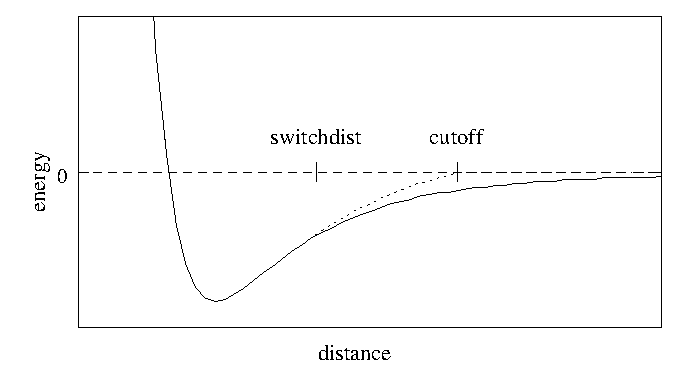
\psfig{file=figures/switching.eps}}
  \caption[Graph of van der Waals potential with and without switching]
  {\small Graph of van der Waals potential with and without the
  application of the switching function.  With the switching function
  active, the potential is smoothly reduced to 0 at the cutoff distance.
  Without the switching function, there is a discontinuity where the
  potential is truncated.}
  \label{fig:switching}
\end{figure}

The details of the switching function are given in the \PG.
The switching function used is based on the X-PLOR switching
function.  The parameter {\tt switchdist} specifies the distance
at which the switching function should start taking effect to
bring the van der Waals potential to 0 smoothly at the cutoff distance.  
Thus, the value of {\tt switchdist} must always be less than that 
of {\tt cutoff}.


\subsubsection{Non-bonded electrostatic interactions}
The handling of electrostatics is slightly
more complicated due to the incorporation of multiple timestepping for full
electrostatic interactions.  There are two cases to consider, one where
full electrostatics is employed and the other where electrostatics
are truncated at a given distance.
\prettypar
First let us consider the latter case, where electrostatics are truncated at
the cutoff distance.  Using this scheme, all electrostatic interactions
beyond a specified distance are ignored, or assumed to be zero.  If
{\tt switching} is set to {\tt on}, rather than having a discontinuity
in the potential
at the cutoff distance, a shifting function is applied to the electrostatic
potential as shown in Figure \ref{fig:shifting}.  As this figure shows, the
shifting function shifts the entire potential curve so that the curve
intersects the x-axis at the cutoff distance.  This shifting function
is fully described in the \PG\ and is based on the
shifting function used by X-PLOR.

\begin{figure}[htb]
  \center{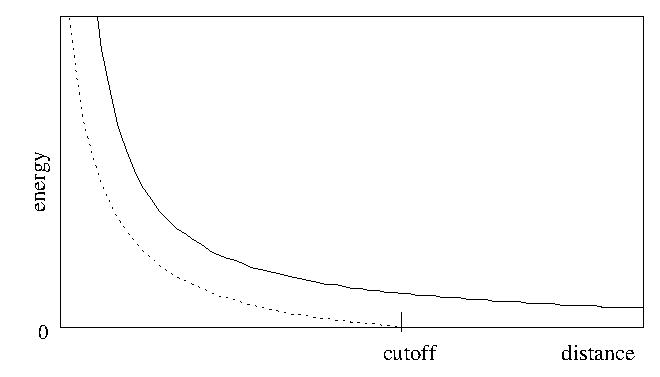
\psfig{file=figures/shifting.eps}}
  \caption[Graph of electrostatic potential with and without shifting function]
  {\small Graph showing an electrostatic potential with and without the
  application of the shifting function.}
  \label{fig:shifting}
\end{figure}

Next, consider the case where full electrostatics are calculated.  In this
case, the electrostatic interactions are not truncated at any distance.  In
this scheme, the {\tt cutoff} parameter has a slightly different meaning
for the electrostatic interactions --- it represents
the {\it local interaction distance\/}, or distance within which electrostatic
pairs will be directly calculated every timestep.  Outside of this distance,
interactions will be calculated only periodically.  These forces
will be applied using a multiple timestep integration scheme as described in
Section \ref{section:fmadesc}.

\begin{figure}[htb]
  \center{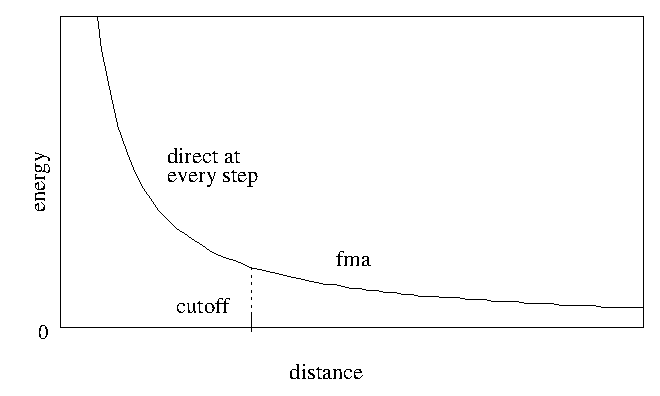
\psfig{file=figures/fmaOn.eps}}
  \caption[Graph of electrostatic split between short and long range forces]
  {\small Graph showing an electrostatic potential 
  when full electrostatics are used within \NAMD, 
  with one curve portion calculated directly 
  and the other calculated using DPMTA.}
  \label{fig:fmaOn}
\end{figure}

\subsubsection{Nonbonded interaction distance-testing}
The last critical parameter for non-bonded
interaction calculations is the parameter {\tt pairlistdist}.  To reduce the
cost of performing the non-bonded interactions, \NAMD\ 1.X used a {\it non-bonded
pair list} which contained all pairs of atoms for which
non-bonded interactions
should be calculated.  Performing the search for pairs of atoms that
should have their interactions calculated is an expensive operation.  Thus,
the pair list is only calculated periodically, once per cycle.   Unfortunately,
pairs of atoms move relative to each other during the steps between preparation
of the pair list.  Because of this, if the pair list were built to include
only
those pairs of atoms that are within the cutoff distance
when the list is generated, it would
be possible 
for atoms to drift closer together
than the cutoff distance during subsequent timesteps and yet not
have their non-bonded interactions calculated.  
\prettypar
Let us consider a concrete example to better understand this.  Assume that the
pairlist is built once every ten timesteps and that the cutoff
distance is 8.0 \AA.  Consider a pair
of atoms A and B that are 8.1 \AA\ apart when the pairlist is built.
If the pair list
includes only those atoms within the cutoff distance, this pair would not
be included in the list.  Now assume that after five timesteps, atoms
A and B have moved to only 7.9 \AA\ apart.  A and B are now within the
cutoff distance of each other, and should have their
non-bonded interactions calculated.
However, because the non-bonded interactions are based solely on the pair list
and the pair list will not be rebuilt for another five timesteps, this pair
will be ignored for five timesteps causing energy not to be conserved 
within the system.  
\prettypar
To avoid this problem, the parameter {\tt pairlistdist} allowed the user
to specify a distance greater than the {\tt cutoff} distance for pairs
to be included in the pair list, as shown in Figure \ref{fig:pairlistdist}.
Pairs that are included in the pair list but are outside the cutoff distance
are simply ignored.  So in the above example, if the {\tt pairlistdist}
were set to $10.0$ \AA, then 
the atom pair A and B would be included in the pair list, even though
the pair would initially be ignored because they are further apart than
the cutoff distance.  As the pair moved closer and entered the cutoff
distance, because the pair was already in the pair list, the non-bonded
interactions would immediately be calculated and energy conservation
would be preserved.  The value of {\tt pairlistdist} should be chosen
such that no atom pair moves more than 
$\mbox{{\tt pairlistdist}}-\mbox{{\tt cutoff}}$ 
in one cycle.  This will insure energy conservation.

\begin{figure}[htb]
  \center{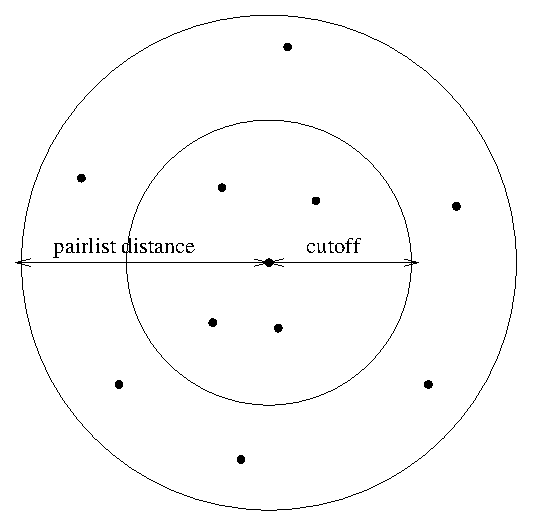
\psfig{file=figures/pairlistdist.eps}}
  \caption[Example of cutoff and pairlist distance uses]
  {{\small Depiction of the difference between the cutoff distance and the
  pair list distance.  The pair list distance specifies a sphere that is
  slightly larger than that of the cutoff so that pairs are allowed to
  move in and out of the cutoff distance without causing energy conservation
  to be disturbed.}}
  \label{fig:pairlistdist}
\end{figure}

NAMD 2.X eliminated the explicit use of pairlists in order to reduce memory usage in light of equally efficient distance-testing algorithms.
Specifically, it was realized that building a pairlist on top of the existing spatial decomposition was only marginally more efficient than actually testing atom distances at every timestep given efficient methods for dealing with nonbonded exclusions.
The {\tt pairlistdist} parameter now serves the same function, but is instead used to determine the minimum patch size.
Unless the {\tt splitPatch} parameter is explicitly set to {\tt position}, hydrogen atoms will be placed on the same patch as the ``mother atom'' to which they are bonded.
These {\em hydrogen groups} are then distance tested against each other using only a cutoff increased by the the value of the {\tt hgroupCutoff} parameter.
The size of the patches is also increased by this amount.
\NAMD\ functions correctly even if a hydrogen atom and its mother atom are separated by more than half of {\tt hgroupCutoff} by breaking that group into its individual atoms for distance testing.
Warning messages are printed if an atom moves outside of a safe zone surrounding the patch to which it is assigned, indicating that {\tt pairlistdist} should be increased in order for forces to be calculated correctly and energy to be conserved.

\subsection{Full electrostatic integration}
\label{section:fmadesc}

To further reduce the cost of computing full electrostatics, 
\NAMD\ uses a multiple timestepping integration scheme.  In this scheme, 
the total force acting on each atom is broken into two pieces, a quickly varying local 
component and a slower long range component.  
The local force component is defined in terms of a {\it splitting function}.  The local force component consists of all bonded and van der Waals interactions
as well as that portion of electrostatic interactions for pairs that are separated by less than the local interaction distance determined by the splitting function.  
The long range component consists only of 
electrostatic interactions outside of the local interaction distance.
Since the long range forces are slowly varying, they are not evaluated
every timestep.  Instead, they are evaluated every $k$ timesteps, and
each set of $k$ timesteps is referred to as a $cycle$.
The value of $k$ is specified by the \NAMD\ parameter
{\tt stepspercycle}.  
An impulse of $k$ times the long range force is applied to the system
every $k$ timesteps (i.e., the r-RESPA integrator is used).
For appropriate values of $k$,
it is believed that the error introduced by this infrequent evaluation
is modest compared to the error already incurred by the use of the numerical
(Verlet) integrator.  
%The performance of \NAMD\ with the use of DPMTA to provide 
%full electrostatics approximately doubles the 
%run time of a simulation as compared to \NAMD\ with an 
%$8.0$ \AA\ electrostatic cutoff.  
Improved methods for incorporating these long range forces
are currently being investigated, 
with the intention of improving accuracy as well as 
reducing the frequency of long range force evaluations.  
\prettypar
In the scheme described above, the van der Waals forces are still 
truncated at the local interaction distance.  
Thus, the van der Waals cutoff distance 
forms a lower limit to the local interaction distance.  While this is
believed to be sufficient, there are investigations underway to remove
this limitation and provide full van der Waals calculations in 
${\mathcal O}(N)$ time as well.  


\subsection{\NAMD\ configuration parameters}
\label{section:config_basic}

\subsubsection{Timestep parameters}

\begin{itemize}
\item
\NAMDCONF{numsteps}{number of timesteps}{positive integer}
{\label{param:numsteps}
%% This parameter is {\it required\/} for every simulation.
The number of simulation timesteps to be performed.  
An integer greater than 0 is acceptable.  
The total amount of simulation 
time is $\mbox{{\tt numsteps}} \times \mbox{{\tt timestep}}$.}

\item
\NAMDCONFWDEF{timestep}{timestep size (fs)}{non-negative decimal}{1.0}
{The timestep size to use when integrating each step of the simulation.  
The value is specified in femtoseconds.}

\item
\NAMDCONFWDEF{firsttimestep}{starting timestep value}{non-negative integer}{0}
{The number of the first timestep.  This value is typically used only 
when a simulation is a continuation of a previous simulation.  In this 
case, rather than having the timestep restart at 0, a specific timestep 
number can be specified.}

\item
\NAMDCONFWDEF{stepspercycle}{timesteps per cycle}{positive integer}{20}
{Number of timesteps in each cycle.  Each cycle represents the number 
of timesteps between pairlist generation and atom reassignment.  
If full electrostatics are active, it is also the number of timesteps 
between full electrostatic evaluation unless {\tt fullElectFrequency} is
also specified.  
It is recommended that {\tt stepspercycle} ({\tt fullElectFrequency}) be chosen so that 
the product of {\tt stepspercycle} and {\tt timestep} does 
not exceed $4.0$ unless {\tt rigidBonds all} is specified, 
in which case the upper limit is perhaps doubled.  
For more details on the 
use of full electrostatics, see Section \ref{section:fmadesc}.  
For more details
on non-bonded force evaluation and pairlist generation, see
Section \ref{section:electdesc}.}


\end{itemize}

\subsubsection{Simulation space partitioning}

\begin{itemize}
%\item
%\NAMDCONF{eleccutoff}%
%{local interaction distance for electrostatic calculations (\AA)}%
%{positive decimal}%
%{If DPMTA is active, this distance defines the local interaction length
%for the DPMTA algorithm.
%Otherwise, this value specifies the distance at which
%electrostatic interactions are truncated.
%If {\tt eleccutoff} is defined, it supersedes {\tt cutoff}.
%If {\tt eleccutoff} is not defined, then \verb }cutoff} {\em must}
%be defined.
%See Section \ref{section:electdesc} for a further discussion
%of this configuration value.}

%\item
%\NAMDCONF{vdwcutoff}%
%{local interaction distance for van der Waals calculations (\AA)}%
%{positive decimal}%
%{This value specifies the distance at which
%van der Waals interactions are truncated.
%If {\tt vdwcutoff} is defined, it supersedes {\tt cutoff}.
%If {\tt vdwcutoff} is not defined, then \verb }cutoff} {\em must}
%be defined.
%See Section \ref{section:electdesc} for a further discussion
%of this configuration value.}

\item
\NAMDCONF{cutoff}
{local interaction distance common to both electrostatic 
and van der Waals calculations (\AA)}
{positive decimal}
{%This value can substitute for either {\tt eleccutoff}
%or {\tt vdwcutoff} if either of those is undefined.
See Section \ref{section:electdesc} for more information.}

\item
\NAMDCONFWDEF{switching}{use switching function?}{{\tt on} or {\tt off}}
{{\tt off}}
{If {\tt switching} is
specified to be {\tt off}, then a truncated cutoff is performed.
If {\tt switching} is turned {\tt on}, then smoothing functions
are applied to both the electrostatics and van der Waals forces.
For a complete description of the non-bonded force parameters see
Section \ref{section:electdesc}.  If {\tt switching} is set to
{\tt on}, then {\tt switchdist} must also be defined.}

%\item
%\NAMDCONF{elecswitchdist}{distance at which to activate switching function for %electrostatic calculations (\AA)}{positive decimal $\leq$ {\tt eleccutoff}}
%{Distance at which the switching function
%used to smooth the truncation of
%electrostatic forces should begin to take effect.  
%This parameter only has meaning if {\tt switching} is 
%set to {\tt on}.  
%The value of {\tt elecswitchdist} must be less than
%or equal to the value of {\tt eleccutoff}, since the switching function
%is only applied on the range from {\tt elecswitchdist} to {\tt eleccutoff}.
%If {\tt elecswitchdist} is defined, it supersedes {\tt switchdist}.
%If {\tt elecswitchdist} is not defined and {\tt switching} is
%{\tt on}, then \verb }switchdist} {\em must} be defined.
%For a complete description of the non-bonded force parameters, see
%Section \ref{section:electdesc}.
%}

%\item
%\NAMDCONF{vdwswitchdist}%
%{distance at which to activate switching function 
%for van der Waals calculations (\AA)}%
%{positive decimal $\leq$ {\tt vdwcutoff}}%
%{Distance at which the switching function
%used to smooth the truncation of
%van der Waals forces should begin to take effect.  
%This parameter only has meaning if {\tt switching} is 
%set to {\tt on}.  
%The value of {\tt vdwswitchdist} must be less than
%or equal to the value of {\tt vdwcutoff}, since the switching function
%is only applied on the range from {\tt vdwswitchdist} to {\tt vdwcutoff}.
%If {\tt vdwswitchdist} is defined, it supersedes {\tt switchdist}.
%If {\tt vdwswitchdist} is not defined and {\tt switching} is
%{\tt on}, then \verb }switchdist} {\em must} be defined.
%For a complete description of the non-bonded force parameters, see
%Section \ref{section:electdesc}.
%}

\item
\NAMDCONF{switchdist}
{distance at which to activate switching function 
for electrostatic and van der Waals calculations (\AA)}
{positive decimal $\leq$ {\tt cutoff}}
{Distance at which the switching function
should begin to take effect.  
This parameter only has meaning if {\tt switching} is 
set to {\tt on}.  
The value of {\tt switchdist} must be less than
or equal to the value of {\tt cutoff}, since the switching function
is only applied on the range from {\tt switchdist} to {\tt cutoff}.  
For a complete description of the non-bonded force parameters see
Section \ref{section:electdesc}.}

\item
\NAMDCONFWDEF{pairlistdist}
{distance between pairs for inclusion in pair lists (\AA)}
{positive decimal $\geq$ {\tt cutoff}}
{{\tt cutoff}}
{
A pair list is generated each cycle, 
containing pairs of atoms for which 
electrostatics and van der Waals interactions will be calculated.
This parameter is used when {\tt switching} is set to {\tt on} to
specify the allowable distance between atoms for inclusion in the
pair list.  
This parameter is equivalent to the X-PLOR parameter {\tt CUTNb}.
If no atom moves more than {\tt pairlistdist}$-${\tt cutoff} during
one cycle, then there will be no jump in electrostatic or van der
Waals energies when the next pair list is built.  Since such a jump
is unavoidable when truncation is used, this parameter may only
be specified when {\tt switching} is set to {\tt on}.  If this
parameter is not specified and {\tt switching} is set to {\tt on},
the value of {\tt cutoff} is used.  
A value of at least one greater than {\tt cutoff} is recommended.  
}

\item
\NAMDCONFWDEF{splitPatch}
{how to assign atoms to patches}
{{\tt position} or {\tt hydrogen}}
{{\tt hydrogen}}
{
When set to {\tt hydrogen}, hydrogen atoms are kept on the same patch as their parents, allowing faster distance checking and rigid bonds.
}

\item
\NAMDCONFWDEF{hgroupCutoff (\AA)}
{used for group-based distance testing}
{positive decimal}
{2.5}
{
This should be set to twice the largest distance which will ever occur between a hydrogen atom and its mother.  Warnings will be printed if this is not the case.  This value is also added to the margin.
}

\item
\NAMDCONFWDEF{margin}
{extra length in patch dimension (\AA)}{positive decimal}{1.0}
{An internal tuning parameter used in determining the size of the cubes 
of space with which \NAMD\ uses to partition the system.  The value of 
this parameter will not change the physical results of the simulation.  
For more details about this parameter see the \PG.  
Unless you are very motivated to get the {\it very} best 
possible performance, just leave this value at the default.}

%\item
%\NAMDCONFWDEF{plMarginCheck}%
%{perform pairlist margin check?}{{\tt yes} or {\tt no}}{{\tt no}}%
%{\label{param:margincheck}
%If this parameter is activated, a check will be performed during 
%each timestep to detect atoms that may have violated the margin 
%between the {\tt pairlistdist} and {\tt cutoff} distances.  
%Such violations will be output by \NAMD.}

\end{itemize}

\subsubsection{Basic dynamics}

\begin{itemize}
\item
\NAMDCONF{exclude}
{exclusion policy to use}
{{\tt none}, {\tt 1-2}, {\tt 1-3}, {\tt 1-4}, or {\tt scaled1-4}}
{\label{param:exclude}
%% This parameter is {\it required\/} for every simulation.
This parameter specifies which pairs of bonded atoms should
be excluded from non-bonded
interactions.  With the value of {\tt none}, no bonded pairs of atoms 
will be excluded.  With the value of {\tt 1-2}, all atom pairs that
are directly connected via a linear bond will be excluded.  With the
value of {\tt 1-3}, all {\tt 1-2} pairs will be excluded along with
all pairs of atoms that are bonded to a common
third atom (i.e., if atom A is bonded to atom B and atom B is bonded
to atom C, then the atom pair A-C would be excluded).
With the value of {\tt 1-4}, all {\tt 1-3} pairs will be excluded along
with all pairs connected by a set of two bonds (i.e., if atom A is bonded
to atom B, and atom B is bonded to atom C, and atom C is bonded to
atom D, then the atom pair A-D would be excluded).  With the value
of {\tt scaled1-4}, all {\tt 1-3} pairs are excluded and all pairs
that match the {\tt 1-4} criteria are modified.  The electrostatic
interactions for such pairs are modified by the constant factor
defined by {\tt 1-4scaling}.  
The van der Waals interactions are modified
by using the special 1-4 parameters defined in the parameter files.}

\item
\NAMDCONF{temperature}{initial temperature (K)}{positive decimal}
{\label{param:temperature}
Initial temperature value for the system.  
Using this option will generate a random
velocity distribution for the initial velocities 
for all the atoms such that the system 
is at the desired temperature.  
Either the {\tt temperature} 
or the {\tt velocities}/{\tt binvelocities}
option must be defined to determine an initial set of velocities.  
Both options cannot be used together.}

\item
\NAMDCONFWDEF{COMmotion}{allow center of mass motion?}
{{\tt yes} or {\tt no}}{{\tt no}}
{
Specifies whether or not motion of 
the center of mass of the entire system is allowed.  
If this option is set to {\tt no}, the initial velocities of the system 
will be adjusted to remove center of mass motion of the system.
Note that this does not preclude later center-of-mass motion due to 
external forces such as random noise in Langevin dynamics, boundary
potentials, and harmonic restraints.}

\item
\NAMDCONFWDEF{dielectric}{dielectric constant for system}
{decimal $\geq$ 1.0}{1.0}
{Dielectric constant for the system.  A value of 1.0 implies no modification
of the electrostatic interactions.  Any larger value will lessen the
electrostatic forces acting in the system.}

\item
\NAMDCONFWDEF{1-4scaling}{scaling factor for 1-4 interactions}
{0 $\leq$ decimal $\leq$ 1}{1.0}
{Scaling factor for 1-4 interactions.  This factor is only used when the
{\tt exclude} parameter is set to {\tt scaled1-4}.  In this case, this
factor is used to modify the electrostatic interactions between 1-4 atom
pairs.  If the {\tt exclude} parameter is set to anything but 
{\tt scaled1-4}, this parameter has no effect regardless of its value.}

\item
\NAMDCONFWDEF{seed}{random number seed}{positive integer}
{pseudo-random value based on current UNIX clock time}
{Number used to seed the random number generator 
if {\tt temperature} or {\tt langevin} is selected.  This can be
used so that consecutive simulations produce the same results.
If no value is specified, \NAMD\ will choose a pseudo-random
value based on the current UNIX clock time.  The random number
seed will be output during the simulation startup so that
its value is known and can be reused for subsequent simulations.
Note that if Langevin dynamics are used in a parallel simulation 
(i.e., a simulation using more than one processor) 
even using the same seed will {\it not} guarantee reproducible results.
}

\item
\NAMDCONFWDEF{rigidBonds}{controls if and how ShakeH is used}{{\tt none},
{\tt water}, {\tt all}}{{\tt none}} 
{When {\tt rigidBonds} is {\tt all}, the bond between each hydrogen
and its mother atom is fixed to the nominal bond length given in the
parameter file.  When {\tt water} is selected, only the bonds between
the hydrogens and the oxygen in water molecules are constrained.  
For the default case {\tt none}, no lengths are constrained.
}

\item
\NAMDCONFWDEF{rigidTolerance}{allowable bond-length error for ShakeH (\AA)}
{positive decimal}{0.00001}
{
The ShakeH algorithm is assumed to have converged when all constrained
bonds differ from the nominal bond length by less than this amount.
}

\item
\NAMDCONFWDEF{rigidIterations}{maximum ShakeH iterations}{positive integer}{100}
{
The maximum number of iterations ShakeH will perform before giving up
on constraining the bond lengths.  If the bond lengths do not
converge, a warning message is printed, and the atoms are left at the
final value achieved by ShakeH.  
Although the default value is 100, 
convergence is usually reached after fewer than 10 iterations.
}

\end{itemize}

\subsubsection{DPMTA parameters}

These parameters control the options to DPMTA, an algorithm
used to provide full electrostatic interactions.  DPMTA is a
modified version of the FMA (Fast Multipole Algorithm) and, 
unfortunately, most of the parameters still refer to FMA
rather than DPMTA for historical reasons.  Don't be confused!
\prettypar
For a further description of how exactly full electrostatics
are incorporated into \NAMD, see Section \ref{section:fmadesc}.
For a greater level of detail about DPMTA and the specific
meaning of its options, see the DPMTA distribution which is
available via anonymous FTP from the site {\tt ftp.ee.duke.edu}
in the directory {\tt /pub/SciComp/src}.

\begin{itemize}

\item
\NAMDCONFWDEF{FMA}{use full electrostatics?}{{\tt on} or {\tt off}}{{\tt off}}
{Specifies whether or not 
the DPMTA algorithm from Duke University should be used 
to compute the full electrostatic interactions.  If set to 
{\tt on}, DPMTA will be used with a multiple timestep integration scheme 
to provide full electrostatic interactions as detailed in Section 
\ref{section:fmadesc}. }

\item
\NAMDCONFWDEF{FMALevels}{number of levels to use in multipole expansion}{positive integer}{5}
{Number of levels to use for the multipole expansion.  This parameter
is only used if {\tt FMA} is set to {\tt on}.  
A value of 4 should be sufficient for systems with less than 10,000 atoms.  
A value of 5 or greater should be used for larger systems. }

\item
\NAMDCONFWDEF{FMAMp}{number of multipole terms to use for FMA}{positive integer}{8}
{Number of terms to use in the multipole expansion.  
This parameter is only used if {\tt FMA} is set to {\tt on}.  
If the {\tt FMAFFT} is set to {\tt on}, then this value must 
be a multiple of 4.  The default value of 8 should be suitable
for most applications.}

\item
\NAMDCONFWDEF{FMAFFT}{use DPMTA FFT enhancement?}{{\tt on} or {\tt off}}{{\tt on}}
{Specifies whether or not the DPMTA code should use the FFT enhancement 
feature.  This parameter is only used if {\tt FMA} is set to {\tt on}.  
If {\tt FMAFFT} is set to {\tt on}, the value of {\tt FMAMp} must be 
set to a multiple of 4.  
This feature offers substantial benefits only for values 
of {\tt FMAMp} of 8 or greater.  This feature will substantially 
increase the amount of memory used by DPMTA.}

%%  REMOVE THIS AS A DOCUMENTED FEATURE.  WE USE stepspercycle INSTEAD.  
%%
%%  \item
%%  \NAMDCONF{FMAfrequency}{number of timesteps between DPMTA calculations}{positive integer}
%%  {This parameter specifies the number of timesteps between each
%%  invocation of the DPMTA algorithm.}

\item
\NAMDCONFWDEF{FMAtheta}{DPMTA theta parameter (radians)}{decimal}{0.715}
{This parameter specifies the value of the theta parameter
used in the DPMTA calculation.  The default value is based on
recommendations by the developers of the code.}

\item
\NAMDCONFWDEF{FMAFFTBlock}{blocking factor for FMA FFT}{positive integer}{4}
{The blocking factor for the FFT enhancement to DPMTA.
This parameter is only used if both {\tt FMA} and {\tt FMAFFT} 
are set to {\tt on}.  The default value of 4 should be suitable
for most applications.}

\end{itemize}

\subsubsection{DPME parameters}

DPME stands for Distributed Particle Mesh Ewald and is an efficient
full electrostatics method for use with periodic boundary conditions.
None of the parameters should affect energy conservation, although they may affect the accuracy of the results and momentum conservation.

\begin{itemize}

\item
\NAMDCONFWDEF{PME}{Use particle mesh Ewald for electrostatics?}{{\tt yes} or {\tt no}}{{\tt no}}
{Turns on DPME.}

\item
\NAMDCONFWDEF{PMETolerance}{PME direct space tolerance}{positive decimal}{$10^{-6}$}
{Affects the value of the Ewald coefficient and the overall accuracy of the results.}

\item
\NAMDCONFWDEF{PMEInterpOrder}{PME interpolation order}{positive integer}{4 (cubic)}
{Charges are interpolated onto the grid and forces are interpolated off using this many points, equal to the order of the interpolation function plus one.}

\item
\NAMDCONF{PMEGridSizeX}{PME grid in x dimension}{positive integer}
{The grid size partially determines the accuracy and efficiency of DPME.
For speed, {\tt PMEGridSizeX} should have only small integer factors (2, 3 and 5).}

\item
\NAMDCONF{PMEGridSizeY}{PME grid in y dimension}{positive integer}
{The grid size partially determines the accuracy and efficiency of DPME.
For speed, {\tt PMEGridSizeY} should have only small integer factors (2, 3 and 5).}

\item
\NAMDCONF{PMEGridSizeZ}{PME grid in z dimension}{positive integer}
{The grid size partially determines the accuracy and efficiency of DPME.
For speed, {\tt PMEGridSizeZ} should have only small integer factors (2, 3 and 5).}

\end{itemize}

\subsubsection{Full direct parameters}

The direct computation of electrostatics 
is not intended to be used during 
real calculations, but rather as a testing or 
comparison measure.  Because of the ${\mathcal O}(N^2)$ 
computational complexity for performing 
direct calculations, this is {\it much} 
slower than using DPMTA or DPME to compute full 
electrostatics for large systems.
In the case of periodic boundary conditions,
the nearest image convention is used rather than a
full Ewald sum.

\begin{itemize}

\item
\NAMDCONFWDEF{FullDirect}{calculate full electrostatics directly?}{{\tt yes} or {\tt no}}{{\tt no}}
{Specifies whether or not direct computation of 
full electrostatics should be performed.}

\end{itemize}

\subsubsection{Multiple timestep parameters}

One of the areas of current research being studied using \NAMD\ is the
exploration of better methods for performing multiple timestep integration.
The parameters in this Section are part of this exploration.  These parameters
are still rather experimental and are not fully documented yet, but the
brave at heart may try them.  By default, the naive scheme described
in the \PG\ is used.

\begin{itemize}

\item
\NAMDCONFWDEF{fullElectFrequency}{number of timesteps between DPMTA calculations}{positive integer factor of {\tt stepspercycle}}{{\tt stepspercycle}}
{This parameter specifies the number of timesteps between each full electrostatics evaluation.
It is recommended that {\tt fullElectFrequency} be chosen so that 
the product of {\tt fullElectFrequency} and {\tt timestep} does 
not exceed $4.0$ unless {\tt rigidBonds all} is specified, 
in which case the upper limit is perhaps doubled.}

\item
\NAMDCONFWDEF{nonbondedFreq}{timesteps between nonbonded evaluation}{positive integer factor of {\tt fullElectFrequency}}{1}
{This parameter specifies how often short-range nonbonded interactions should be calculated.  Setting {\tt nonbondedFreq} between 1 and {\tt fullElectFrequency} allows triple timestepping where, for example, one could evaluate bonded forces every 1 fs, short-range nonbonded forces every 2 fs, and long-range electrostatics every 4 fs.} 

\item
\NAMDCONFWDEF{MTSAlgorithm}{MTS algorithm to be used}{{\tt verletI}}{{\tt verletI}}
{Specifies the multiple timestep algorithm used to integrate the 
long and short range forces.  {\tt verletI} is the same as r-RESPA.}

\item
\NAMDCONFWDEF{longSplitting}{how should long and short range forces be split?}{{\tt xplor}, {\tt c1}}{{\tt c1}}
{Specifies the method used to split electrostatic forces between long 
and short range potentials.  
The {\tt xplor} option uses the X-PLOR shifting function, 
and the {\tt c1} splitting uses 
the following $C^1$ continuous shifting 
function \mycite{Humphreys \ETAL}{HUMP94}:  
\begin{list}{}{}
\item
$SW(r_{ij}) = 0$ if $|{{\vec{r}}_{ij}}| > R_{\mathit off}$
\item
$SW(r_{ij}) = 1$ if $|{{\vec{r}}_{ij}}| \leq R_{\mathit on}$
\item
$SW(r_{ij}) = \frac{ {\left({R_{\mathit off}}^2 - {r_{ij}}^2\right)}^2
\left({R_{\mathit off}}^2 + 2{r_{ij}}^2 - 3{R_{\mathit on}}^2\right)}
{{\left({R_{\mathit off}}^2 - {R_{\mathit on}}^2\right)}^3}$
if $R_{\mathit off} > |{{\vec{r}}_{ij}}| \geq R_{\mathit on}$
\end{list}
}
where
\begin{list}{}{}
\item
$R_{\mathit on}$ is a constant defined using the configuration value 
{\tt switchdist} 
\item
$R_{\mathit off}$ is specified using the configuration value {\tt cutoff}
\end{list}

\end{itemize}



% Additional simulation parameters
\newpage

\section{Additional Simulation Parameters}
\label{section:add}

\subsection{Constraints and Restraints}
\label{section:config_add}

\subsubsection{Harmonic constraint parameters}

The following describes the parameters for the 
harmonic constraints feature of \NAMD.  Actually, this feature 
should be referred to as harmonic restraints rather than 
constraints, but for historical reasons the terminology of 
harmonic constraints has been carried over from X-PLOR.  
This feature allows a harmonic restraining force to be applied 
to any set of atoms in the simulation.

\begin{itemize}

\item
\NAMDCONFWDEF{constraints}{are constraints active?}{{\tt on} or {\tt off}}{{\tt off}}
{Specifies whether or not harmonic constraints are active.  If it 
is set to {\tt off}, then no harmonic constraints are computed.  
If it is set to {\tt on}, then 
harmonic constraints are calculated using the values specified 
by the parameters {\tt consref}, {\tt conskfile}, {\tt conskcol}, 
and {\tt consexp}.}

\item
\NAMDCONFWDEF{consexp}{exponent for harmonic constraint energy function}{positive, even integer}{2}
{Exponent to be use in the harmonic constraint energy function.  
This value must be a positive integer, and only even values really make 
sense.  This parameter is used only if {\tt constraints} is set to 
{\tt on}.}

\item
\NAMDCONFWDEF{consref}{PDB file containing constraint reference positions}{UNIX file name}{{\tt coordinates}}
{PDB file to use for reference positions for harmonic constraints.  
Each atom that has an active constraint will be constrained about 
the position specified in this file.  If no value is given and constraints 
are active, then the same PDB file specified by {\tt coordinates} will be 
used instead, constraining atoms about their initial positions.}

\item
\NAMDCONFWDEF{conskfile}{PDB file containing force constant values}{UNIX filename} {{\tt coordinates}}
{PDB file to use for force constants for 
harmonic constraints.  
If this parameter is not specified, then 
the PDB file containing initial coordinates specified by 
{\tt coordinates} is used.}

\item
\NAMDCONFWDEF{conskcol}{column of PDB file containing force constant}{{\tt X}, {\tt Y}, {\tt Z}, {\tt O}, or {\tt B}}{{\tt O}}
{Column of the PDB file to use for the harmonic constraint force constant.
This parameter may specify any of the floating point fields of the PDB file, 
either X, Y, Z, occupancy, or beta-coupling (temperature-coupling).  
Regardless of which column is used, a value of 0 indicates that the atom 
should not be constrained.  
Otherwise, the value specified is used as the force constant for 
that atom's restraining potential.}

\item
\NAMDCONFWDEF{selectConstraints}{Restrain only selected Cartesian components of the coordinates?}{{\tt on} or {\tt off}}{{\tt off}}
{This option is useful to restrain the positions of atoms to a plane or a line in space. If active,
 this option will ensure that only selected Cartesian components of the coordinates are restrained.
 E.g.: Restraining the positions of atoms to their current z values with no restraints
 in x and y will allow the atoms to move in the x-y plane while retaining their original z-coordinate.
 Restraining the x and y values will lead to free motion only along the z coordinate.}

\item
\NAMDCONFWDEF{selectConstrX}{Restrain X components of coordinates}{{\tt on} or {\tt off}}{{\tt off}}
{Restrain the Cartesian x components of the positions.}
\item
\NAMDCONFWDEF{selectConstrY}{Restrain Y components of coordinates}{{\tt on} or {\tt off}}{{\tt off}}
{Restrain the Cartesian y components of the positions.}
\item
\NAMDCONFWDEF{selectConstrZ}{Restrain Z components of coordinates}{{\tt on} or {\tt off}}{{\tt off}}
{Restrain the Cartesian z components of the positions.}

\end{itemize}

\subsubsection{Fixed atoms parameters}

Atoms may be held fixed during a simulation.  \NAMD\ avoids calculating most interactions in which all affected atoms are fixed unless {\tt fixedAtomsForces} is specified.

\begin{itemize}

\item
\NAMDCONFWDEF{fixedAtoms}{are there fixed atoms?}{{\tt on} or {\tt off}}{{\tt off}}
{Specifies whether or not fixed atoms are present.} 

\item
\NAMDCONFWDEF{fixedAtomsForces}{are forces between fixed atoms calculated?}{{\tt on} or {\tt off}}{{\tt off}}
{Specifies whether or not forces between fixed atoms are calculated.  This option is required for constant pressure or to turn fixed atoms off in the middle of a simulation.}

\item
\NAMDCONFWDEF{fixedAtomsFile}{PDB file containing fixed atom parameters}
{UNIX filename}{{\tt coordinates}}
{PDB file to use for the fixed atom flags for each atom.  
If this parameter is not specified, then 
the PDB file specified by {\tt coordinates} is used.}

\item
\NAMDCONFWDEF{fixedAtomsCol}{column of PDB containing fixed atom parameters}
{{\tt X}, {\tt Y}, {\tt Z}, {\tt O}, or {\tt B}}{{\tt O}} 
{Column of the PDB file to use for the containing fixed atom parameters for 
each atom.  The coefficients can be read from any 
floating point column of the PDB file.  
A value of 0 indicates that the atom is not fixed.}

\end{itemize}

\subsection{Energy Minimization}

\subsubsection{Conjugate gradient parameters}

The default minimizer uses a sophisticated conjugate gradient and
line search algorithm with much better performance than the older
velocity quenching method.
The method of conjugate gradients is used to select successive search
directions (starting with the initial gradient) which eliminate
repeated minimization along the same directions.
Along each direction, a minimum is first bracketed (rigorously bounded)
and then converged upon by either a golden section search, or, when
possible, a quadratically convergent method using gradient information.

For most systems, it just works.

\begin{itemize}

\item
\NAMDCONFWDEF{minimization}{Perform conjugate gradient energy minimization?}{{\tt on} or {\tt off}}{{\tt off}}
{Turns efficient energy minimization {\tt on} or {\tt off}.}

\item
\NAMDCONFWDEF{minTinyStep}{first initial step for line minimizer}{positive decimal}{1.0e-6}
{If your minimization is immediately unstable, make this smaller.}

\item
\NAMDCONFWDEF{minBabyStep}{max initial step for line minimizer}{positive decimal}{1.0e-2}
{If your minimization becomes unstable later, make this smaller.}

\item
\NAMDCONFWDEF{minLineGoal}{gradient reduction factor for line minimizer}{positive decimal}{1.0e-4}
{Varying this might improve conjugate gradient performance.}

\end{itemize}

\subsubsection{Velocity quenching parameters}

You can perform energy minimization using a simple quenching
scheme.   While this algorithm is not the most rapidly convergent, it
is sufficient for most applications.  There are only two parameters
for minimization:  one to activate minimization and another
to specify the maximum movement of any atom.  

\begin{itemize}

\item
\NAMDCONFWDEF{velocityQuenching}{Perform old-style energy minimization?}{{\tt on} or {\tt off}}{{\tt off}}
{Turns slow energy minimization {\tt on} or {\tt off}.}

\item
\NAMDCONFWDEF{maximumMove}{maximum distance an atom can move during each step (\AA)}
{positive decimal}
{$0.75\times\mbox{{\tt cutoff}}/\mbox{{\tt stepsPerCycle}}$}
{Maximum distance that an atom can move during any single timestep of
minimization.  This is to insure that atoms do not go flying off into
space during the first few timesteps when the largest energy conflicts
are resolved.}

\end{itemize}

\subsection{Temperature Control and Equilibration}

\subsubsection{Langevin dynamics parameters}

\NAMD\ is capable
of performing Langevin dynamics, where additional damping and
random forces are introduced to the system.  This capability
is based on that implemented in X-PLOR which is detailed
in the X-PLOR {\it User's Manual} \mycite{(Br\"unger, 1992)}{BRUN92b},
although a different integrator is used.

\begin{itemize}

\item
\NAMDCONFWDEF{langevin}{use Langevin dynamics?}{{\tt on} or {\tt off}}{{\tt off}}
{Specifies whether or not Langevin dynamics active.  
If set to {\tt on}, then the parameter {\tt langevinTemp} must be set 
and the parameters {\tt langevinFile} and {\tt langevinCol} can
optionally be set to control the behavior of this feature.} 

\item
\NAMDCONF{langevinTemp}{temperature for Langevin calculations (K)}{positive decimal}
{Temperature to which atoms affected by Langevin dynamics will be adjusted.  
This temperature will be roughly maintained across the affected atoms 
through the addition of friction and random forces.}

\item
\NAMDCONFWDEF{langevinDamping}{damping coefficient for Langevin dynamics (1/ps)}{positive decimal}{per-atom values from PDB file}
{Langevin coupling coefficient to be applied to all atoms (unless {\tt langevinHydrogen} is {\tt off}, in which case only non-hydrogen atoms are affected).
If not given, a PDB file is used to obtain coefficients for each atom (see {\tt langevinFile} and {\tt langevinCol} below).}

\item
\NAMDCONFWDEF{langevinHydrogen}{Apply Langevin dynamics to hydrogen atoms?}{{\tt on} or {\tt off}}{{\tt on}}
{If {\tt langevinDamping} is set then setting {\tt langevinHydrogen} to {\tt off} will turn off Langevin dynamics for hydrogen atoms.  This parameter has no effect if Langevin coupling coefficients are read from a PDB file.}

\item
\NAMDCONFWDEF{langevinFile}{PDB file containing Langevin parameters}
{UNIX filename}{{\tt coordinates}}
{PDB file to use for the Langevin coupling coefficients for each atom.  
If this parameter is not specified, then 
the PDB file specified by {\tt coordinates} is used.}

\item
\NAMDCONFWDEF{langevinCol}{column of PDB from which to read coefficients}
{{\tt X}, {\tt Y}, {\tt Z}, {\tt O}, or {\tt B}}{{\tt O}} 
{Column of the PDB file to use for the Langevin coupling coefficients for 
each atom.  The coefficients can be read from any 
floating point column of the PDB file.  
A value of 0 indicates that the atom will remain unaffected.}

\end{itemize}

\subsubsection{Temperature coupling parameters}

\NAMD\ is capable
of performing temperature coupling, in which forces are added or 
reduced to simulate the coupling of the system to a heat bath 
of a specified temperature.  
This capability is based on that implemented in X-PLOR which is detailed
in the X-PLOR {\it User's Manual} \mycite{(Br\"unger, 1992)}{BRUN92b}.

\begin{itemize}

\item
\NAMDCONFWDEF{tCouple}{perform temperature coupling?}{{\tt on} or {\tt off}}{{\tt off}}
{Specifies whether or not temperature coupling is active.  
If set to {\tt on}, then the parameter {\tt tCoupleTemp} must be set and 
the parameters {\tt tCoupleFile} and {\tt tCoupleCol} can 
optionally be set to control the behavior of this feature.} 

\item
\NAMDCONF{tCoupleTemp}{temperature for heat bath (K)}{positive decimal}
{Temperature to which atoms affected 
by temperature coupling will be adjusted.  
This temperature will be roughly maintained across the affected atoms 
through the addition of forces.}

\item
\NAMDCONFWDEF{tCoupleFile}{PDB file with tCouple parameters}
{UNIX filename}{{\tt coordinates}}
{PDB file to use for the temperature coupling coefficient for each atom.  
If this parameter is not specified, then 
the PDB file specified by {\tt coordinates} is used.} 

\item
\NAMDCONFWDEF{tCoupleCol}{column of PDB from which to read coefficients}
{{\tt X}, {\tt Y}, {\tt Z}, {\tt O}, or {\tt B}}{{\tt O}} 
{Column of the PDB file to use for the temperature coupling coefficient for 
each atom.  This value can be read from any 
floating point column of the PDB file.  
A value of $0$ indicates that the atom will remain unaffected.}

\end{itemize}

\subsubsection{Temperature rescaling parameters}

\NAMD\ allows equilibration of a system by means of temperature 
rescaling.  Using this method, all of the velocities in the system 
are periodically rescaled so that the entire system is set to the 
desired temperature.  The following parameters specify how often 
and to what temperature this rescaling is performed.  

\begin{itemize}

\item
\NAMDCONF{rescaleFreq}{number of timesteps between temperature rescaling}{positive integer}
{The equilibration feature of \NAMD\ is activated by 
specifying the number of timesteps between each temperature rescaling.  
If this value is given, then the {\tt rescaleTemp} parameter must also 
be given to specify the target temperature. }

\item
\NAMDCONF{rescaleTemp}{temperature for equilibration (K)}{positive decimal}
{The temperature to which all velocities will be rescaled
every {\tt rescaleFreq} timesteps.  
This parameter is valid only if {\tt rescaleFreq} has been set.}

\end{itemize}

\subsubsection{Temperature reassignment parameters}

\NAMD\ allows equilibration of a system by means of temperature 
reassignment.  Using this method, all of the velocities in the system 
are periodically reassigned so that the entire system is set to the 
desired temperature.  The following parameters specify how often 
and to what temperature this reassignment is performed.  

\begin{itemize}

\item
\NAMDCONF{reassignFreq}{number of timesteps between temperature reassignment}{positive integer}
{The equilibration feature of \NAMD\ is activated by 
specifying the number of timesteps between each temperature reassignment.
If this value is given, then the {\tt reassignTemp} parameter must also 
be given to specify the target temperature. }

\item
\NAMDCONFWDEF{reassignTemp}{temperature for equilibration (K)}{positive decimal}{{\tt temperature} if set, otherwise none}
{The temperature to which all velocities will be reassigned
every {\tt reassignFreq} timesteps.  
This parameter is valid only if {\tt reassignFreq} has been set.}

\item
\NAMDCONFWDEF{reassignIncr}{temperature increment for equilibration (K)}{decimal}{0}
{In order to allow simulated annealing or other slow heating/cooling protocols, {\tt reassignIncr} will be added to {\tt reassignTemp} after each reassignment.
(Reassignment is carried out at the first timestep.)  The {\tt reassignHold} parameter may be set to limit the final temperature.
This parameter is valid only if {\tt reassignFreq} has been set.}

\item
\NAMDCONF{reassignHold}{holding temperature for equilibration (K)}{positive decimal}
{The final temperature for reassignment when {\tt reassignIncr} is set; {\tt reassignTemp} will be held at this value once it has been reached.
This parameter is valid only if {\tt reassignIncr} has been set.}

\end{itemize}

\subsection{Boundary Conditions}

\subsubsection{Spherical harmonic boundary conditions}

\NAMD\ provides spherical harmonic boundary conditions.  These 
boundary conditions can consist of a single potential or a 
combination of two potentials.
The following parameters are used to define these boundary conditions.  

\begin{itemize}

\item
\NAMDCONFWDEF{sphericalBC}{use spherical boundary conditions?}{{\tt on} or {\tt off}}{{\tt off}}
{Specifies whether or not spherical boundary conditions 
are to be applied to the system.  If 
set to {\tt on}, then {\tt sphericalBCCenter}, {\tt sphericalBCr1} and {\tt sphericalBCk1} 
must be defined, and {\tt sphericalBCexp1}, {\tt sphericalBCr2}, 
{\tt sphericalBCk2}, and {\tt sphericalBCexp2} can optionally be 
defined.}

\item
\NAMDCONF{sphericalBCCenter}{center of sphere (\AA)}{position}
{Location around which sphere is centered.}

\item
\NAMDCONF{sphericalBCr1}{radius for first boundary condition (\AA)}{positive decimal}
{Distance at which the first potential of the boundary conditions takes
effect.  This distance is a radius from the center.}

\item
\NAMDCONF{sphericalBCk1}{force constant for first potential}{non-zero decimal}
{Force constant for the first harmonic potential.  A positive
value will push atoms toward the center, and a negative
value will pull atoms away from the center.}

\item
\NAMDCONFWDEF{sphericalBCexp1}{exponent for first potential}{positive, even integer}{2}
{Exponent for first boundary potential.  The only likely values to
use are 2 and 4.}

\item
\NAMDCONF{sphericalBCr2}{radius for second boundary condition (\AA)}{positive decimal}
{Distance at which the second potential of the boundary conditions takes
effect.  This distance is a radius from the center.
If this parameter is defined, then {\tt spericalBCk2} must also
be defined.}

\item
\NAMDCONF{sphericalBCk2}{force constant for second potential}{non-zero decimal}
{Force constant for the second harmonic potential.  A positive
value will push atoms toward the center, and a negative
value will pull atoms away from the center.}

\item
\NAMDCONFWDEF{sphericalBCexp2}{exponent for second potential}{positive, even integer}{2}
{Exponent for second boundary potential.  The only likely values to
use are 2 and 4.}

\end{itemize}

\subsubsection{Cylindrical harmonic boundary conditions}

\NAMD\ provides cylindrical harmonic boundary conditions.  These 
boundary conditions can consist of a single potential or a 
combination of two potentials.
The following parameters are used to define these boundary conditions.  

\begin{itemize}

\item
\NAMDCONFWDEF{cylindricalBC}{use cylindrical boundary conditions?}{{\tt on} or {\tt off}}{{\tt off}}
{Specifies whether or not cylindrical boundary conditions 
are to be applied to the system.  If 
set to {\tt on}, then {\tt cylindricalBCCenter}, {\tt cylindricalBCr1}, {\tt cylindricalBCl1} and {\tt cylindricalBCk1} 
must be defined, and {\tt cylindricalBCAxis}, {\tt cylindricalBCexp1}, {\tt cylindricalBCr2}, {\tt cylindricalBCl2},
{\tt cylindricalBCk2}, and {\tt cylindricalBCexp2} can optionally be 
defined.}

\item
\NAMDCONF{cylindricalBCCenter}{center of  cylinder (\AA)}{position}
{Location around which cylinder is centered.}

\item
\NAMDCONF{cylindricalBCAxis}{axis of  cylinder (\AA)}{{\tt x}, {\tt y}, or {\tt z}}
{Axis along which cylinder is aligned.}

\item
\NAMDCONF{cylindricalBCr1}{radius for first boundary condition (\AA)}{positive decimal}
{Distance at which the first potential of the boundary conditions takes
effect along the non-axis plane of the cylinder.}

\item
\NAMDCONF{cylindricalBCl1}{distance along cylinder axis for first boundary condition (\AA)}{positive decimal}
{Distance at which the first potential of the boundary conditions takes
effect along the cylinder axis.}

\item
\NAMDCONF{cylindricalBCk1}{force constant for first potential}{non-zero decimal}
{Force constant for the first harmonic potential.  A positive
value will push atoms toward the center, and a negative
value will pull atoms away from the center.}

\item
\NAMDCONFWDEF{cylindricalBCexp1}{exponent for first potential}{positive, even integer}{2}
{Exponent for first boundary potential.  The only likely values to
use are 2 and 4.}

\item
\NAMDCONF{cylindricalBCr2}{radius for second boundary condition (\AA)}{positive decimal}
{Distance at which the second potential of the boundary conditions takes
effect along the non-axis plane of the cylinder.
If this parameter is defined, then {\tt cylindricalBCl2} and {\tt spericalBCk2} must also
be defined.}

\item
\NAMDCONF{cylindricalBCl2}{radius for second boundary condition (\AA)}{positive decimal}
{Distance at which the second potential of the boundary conditions takes
effect along the cylinder axis.
If this parameter is defined, then {\tt cylindricalBCr2} and {\tt spericalBCk2} must also
be defined.}

\item
\NAMDCONF{cylindricalBCk2}{force constant for second potential}{non-zero decimal}
{Force constant for the second harmonic potential.  A positive
value will push atoms toward the center, and a negative
value will pull atoms away from the center.}

\item
\NAMDCONFWDEF{cylindricalBCexp2}{exponent for second potential}{positive, even integer}{2}
{Exponent for second boundary potential.  The only likely values to
use are 2 and 4.}

\end{itemize}


\subsubsection{Periodic boundary conditions}

\NAMD\ provides periodic boundary conditions in 1, 2 or 3 dimensions.
The following parameters are used to define these boundary conditions.  

\begin{itemize}

\item
\NAMDCONFWDEF{cellBasisVector1}{basis vector for periodic boundaries (\AA)}{vector}{0 0 0}
{Specifies a basis vector for periodic boundary conditions.}

\item
\NAMDCONFWDEF{cellBasisVector2}{basis vector for periodic boundaries (\AA)}{vector}{0 0 0}
{Specifies a basis vector for periodic boundary conditions.}

\item
\NAMDCONFWDEF{cellBasisVector3}{basis vector for periodic boundaries (\AA)}{vector}{0 0 0}
{Specifies a basis vector for periodic boundary conditions.}

\item
\NAMDCONFWDEF{cellOrigin}{center of periodic cell (\AA)}{position}{0 0 0}
{When position rescaling is used to control pressure, this location will remain constant.  Also used as the center of the cell for wrapped output coordinates.}

\item
\NAMDCONF{extendedSystem}{XSC file to read cell parameters from}{file name}
{In addition to .coor and .vel output files, \NAMD\ generates a .xsc (eXtended System Configuration) file which contains the periodic cell parameters and extended system variables, such as the strain rate in constant pressure simulations.  Periodic cell parameters will be read from this file if this option is present, ignoring the above parameters.}

\item
\NAMDCONF{XSTfile}{XST file to write cell trajectory to}{file name}
{\NAMD\ can also generate a .xst (eXtended System Trajectory) file which contains a record of the periodic cell parameters and extended system variables during the simulation.  If {\tt XSTfile} is defined, then {\tt XSTfreq} must also be defined.}

\item
\NAMDCONF{XSTfreq}{how often to append state to XST file}{positive integer}
{Like the {\tt DCDfreq} option, controls how often the extended system configuration will be appended to the XST file.}

\item
\NAMDCONFWDEF{wrapWater}{wrap water coordinates around periodic boundaries?}{on or off}{off}
{Coordinates are normally output relative to the way they were read in.  Hence, if part of a molecule crosses a periodic boundary it is not translated to the other side of the cell on output.  This option alters this behavior for water molecules only.}

\item
\NAMDCONFWDEF{wrapAll}{wrap all coordinates around periodic boundaries?}{on or off}{off}
{Coordinates are normally output relative to the way they were read in.  Hence, if part of a molecule crosses a periodic boundary it is not translated to the other side of the cell on output.  This option alters this behavior for all contiguous clusters of bonded atoms.}

\item
\NAMDCONFWDEF{wrapNearest}{use nearest image to cell origin when wrapping coordinates?}{on or off}{off}
{Coordinates are normally wrapped to the diagonal unit cell centered on the origin.  This option, combined with {\tt wrapWater} or {\tt wrapAll}, wraps coordinates to the nearest image to the origin, providing hexagonal or other cell shapes.}

\end{itemize}

\subsection{Pressure Control}

The following options affect all pressure control methods.

\begin{itemize}

\item
\NAMDCONFWDEF{useGroupPressure}{group or atomic quantities}
{{\tt yes} or {\tt no}}{{\tt no}}
{Pressure can be calculated using either the atomic virial and kinetic
energy (the default) or a hydrogen-group based pseudo-molecular
virial and kinetic energy.  The latter fluctuates less and is
required in conjunction with rigidBonds (SHAKE).}

\item
\NAMDCONFWDEF{useFlexibleCell}{anisotropic cell fluctuations}
{{\tt yes} or {\tt no}}{{\tt no}}
{\NAMD\ allows the three orthogonal dimensions of the periodic cell
to fluctuate independently when this option is enabled.}

\item
\NAMDCONFWDEF{useConstantRatio}{constant shape in first two cell dimensions}
{{\tt yes} or {\tt no}}{{\tt no}}
{When enabled, \NAMD\ keeps the ratio of the unit cell in the x-y plane 
constant while allowing fluctuations along all axes.  The {\tt useFlexibleCell} option is required for this option.}

\item
\NAMDCONFWDEF{useConstantArea}{constant area and normal pressure conditions}
{{\tt yes} or {\tt no}}{{\tt no}}
{When enabled, \NAMD\ keeps the dimension of the unit cell in the x-y plane 
constant while allowing fluctuations along the z axis.
This is not currently implemented in Berendsen's method.}

\end{itemize}

\subsubsection{Berendsen pressure bath coupling}

\NAMD\ provides constant pressure simulation using Berendsen's method.  
The following parameters are used to define the algorithm.  

\begin{itemize}

\item
\NAMDCONFWDEF{BerendsenPressure}{use Berendsen pressure bath coupling?}{{\tt on} or {\tt off}}{{\tt off}}
{Specifies whether or not Berendsen pressure bath coupling is active.  
If set to {\tt on}, then the parameters {\tt BerendsenPressureTarget}, {\tt BerendsenPressureCompressibility} and {\tt BerendsenPressureRelaxationTime} must be set 
and the parameter {\tt BerendsenPressureFreq} can
optionally be set to control the behavior of this feature.} 

\item
\NAMDCONF{BerendsenPressureTarget}{target pressure (bar)}{positive decimal}
{Specifies target pressure for Berendsen's method.}

\item
\NAMDCONF{BerendsenPressureCompressibility}{compressibility (bar$^{-1}$)}{positive decimal}
{Specifies compressibility for Berendsen's method.}

\item
\NAMDCONF{BerendsenPressureRelaxationTime}{relaxation time (fs)}{positive decimal}
{Specifies relaxation time for Berendsen's method.}

\item
\NAMDCONFWDEF{BerendsenPressureFreq}{how often to rescale positions}{positive multiple of {\tt nonbondedFrequency} and {\tt fullElectFrequency}}{{\tt nonbondedFrequency} or {\tt fullElectFrequency} if used}
{Specifies number of timesteps between position rescalings for Berendsen's method.}

\end{itemize}

\subsubsection{Nos\'{e}-Hoover Langevin piston pressure control}

\NAMD\ provides constant pressure simulation using a modified Nos\'{e}-Hoover method in which Langevin dynamics is used to control fluctuations in the barostat.
This method should be combined with a method of temperature control, such as Langevin dynamics, in order to simulate the NPT ensemble.
The following parameters are used to define the algorithm.  

\begin{itemize}

\item
\NAMDCONFWDEF{LangevinPiston}{use Langevin piston pressure control?}{{\tt on} or {\tt off}}{{\tt off}}
{Specifies whether or not Langevin piston pressure control is active.  
If set to {\tt on}, then the parameters {\tt LangevinPistonTarget}, {\tt LangevinPistonPeriod}, {\tt LangevinPistonDecay} and {\tt LangevinPistonTemp} must be set.}

\item
\NAMDCONF{LangevinPistonTarget}{target pressure (bar)}{positive decimal}
{Specifies target pressure for Langevin piston method.}

\item
\NAMDCONF{LangevinPistonPeriod}{oscillation period (fs)}{positive decimal}
{Specifies barostat oscillation time scale for Langevin piston method.}

\item
\NAMDCONF{LangevinPistonDecay}{damping time scale (fs)}{positive decimal}
{Specifies barostat damping time scale for Langevin piston method.}

\item
\NAMDCONF{LangevinPistonTemp}{noise temperature (K)}{positive decimal}
{Specifies barostat noise temperature for Langevin piston method.
This should be set equal to the target temperature for the chosen method of temperature control.}

\item
\NAMDCONFWDEF{SurfaceTensionTarget}{Surface tension target (dyn/cm)}
{decimal}{0.0}{Specifies surface tension target.  Must be used with 
{\tt useFlexibleCell} and periodic boundary conditions.  The pressure 
specified in {\tt LangevinPistonTarget} becomes the pressure along the z
axis, and surface tension is applied in the x-y plane.}

\item
\NAMDCONFWDEF{StrainRate}{initial strain rate}{decimal triple (x y z)}
{0. 0. 0.}
{Optionally specifies the initial strain rate for pressure control.
Is overridden by value read from file specified with {\tt extendedSystem}.}

\item
\NAMDCONFWDEF{ExcludeFromPressure}{Should some atoms be excluded from pressure
rescaling?}{{\tt on} or {\tt off}}{{\tt off}}
{Specifies whether or not to exclude some atoms from pressure rescaling.  The
coordinates and velocites of such atoms are not rescaled during constant
pressure simulations, though they do contribute to the virial calculation. 
May be useful for membrane protein simulation.  EXPERIMENTAL.}

\item
\NAMDCONFWDEF{ExcludeFromPressureFile}{File specifying excluded atoms}
{PDB file}{coordinates file}
{PDB file with one column specifying which atoms to exclude from pressure
rescaling.  Specify 1 for excluded and 0 for not excluded.}

\item
\NAMDCONFWDEF{ExcludeFromPressureCol}{Column in PDB file for specifying
excluded atoms}{O, B, X, Y, or Z}{O}
{Specifies which column of the pdb file to check for excluded atoms.}

\end{itemize}

\subsection{Applied Forces and Analysis}

There are several ways to apply external forces to simulations with \NAMD.
These are described below.


\subsubsection{Constant Forces}

NAMD provides the ability to apply constant forces to some atoms.
There are two parameters that control this feature.

\begin{itemize}

\item
\NAMDCONFWDEF{constantforce}{Apply constant forces?}{yes or no}{no}
{Specifies whether or not constant forces are applied.}

\item
\NAMDCONF{consforcefile}{PDB file containing forces to be applied}{UNIX filename}
{
The X, Y, Z and occupancy (O) fields of this file are read to
determine the constant force vector of each atom, which is
(X,Y,Z)*O, in unit of Kcal/(mol*\AA). The occupancy (O) serves as
a scaling factor, which could expand the range of the force
applied. (One may be unable to record very large or very small
numbers in the data fields of a PDB file due to limited space).
Zero forces are ignored.

Specifying {\tt consforcefile} is optional; constant forces may be specifed
or updated between runs by using the consForceConfig command.
}

\end{itemize}


\subsubsection{External Electric Field}

\NAMD\ provides the ability to apply a constant electric field to the molecular
system being simulated.
Energy due to the external field will be reported in the MISC column
and may be discontinuous in simulations using periodic boundary conditions if,
for example, a charged hydrogen group moves outside of the central cell.
There are two parameters that control this feature.

\begin{itemize}

\item
\NAMDCONFWDEF{eFieldOn}{apply electric field?}{{\tt yes} or {\tt no}}{{\tt no}}
{Specifies whether or not an electric field is applied.}

\item
\NAMDCONF{eField}{electric field vector}{vector of decimals (x y z)}
{Vector which describes the electric field to be applied.
Units are ${\rm kcal} / ({\rm mol \; \AA} \; e)$, which is natural for simulations.
This parameter may be changed between {\tt run} commands, allowing a square
wave or other approximate wave form to be applied.}

\end{itemize}


\subsubsection{Moving Constraints}

Moving constraints feature works in conjunction with the Harmonic
Constraints (see an appropriate section of the User's guide).
The reference positions of all constraints
will move according to
\begin{equation}
\label{eq:smdrefpos}
   \vec r(t) \; = \; \vec r_0 \, + \, \vec v t \,.
\end{equation}

A velocity vector $\vec v$ ({\tt movingConsVel}) needs to be specified.

The way the moving constraints work is that the moving reference
position is calculated every integration time step using
Eq.~\ref{eq:smdrefpos}, where $\vec v$ is in \AA/timestep, and $t$ is the
current timestep (i.e., {\tt firstTimestep} plus however many
timesteps have passed since the beginning of \NAMD\ run). Therefore,
one should be careful when restarting simulations to appropriately
update the {\tt firstTimestep} parameter in the \NAMD\ configuration
file or the reference position specified in the reference PDB file.

\noindent {\bf NOTE: } \NAMD\ actually calculates the constraints
potential with $U = k (x-x_0)^d$ and the force with $F = d k (x-x_0)$,
where $d$ is the exponent {\tt consexp}. The result is that if one
specifies some value for the force constant $k$ in the PDB file,
effectively, the force constant is $2 k$ in calculations. This caveat
was removed in SMD feature.

The following parameters describe the parameters for the
moving harmonic constraint feature of \NAMD.

\begin{itemize}

\item
\NAMDCONFWDEF{movingConstraints}{Are moving constraints active}
{{\tt on} or {\tt off}}{{\tt off}}
{Should moving restraints be applied to the system. If set
to {\tt on}, then  {\tt movingConsVel} must be defined.
May not be used with {\tt rotConstraints}.}

\item
\NAMDCONF{movingConsVel}{Velocity of the reference position movement}
{vector in \AA/timestep}
{The velocity of the reference position movement. Gives both absolute
value and direction}

\end{itemize}

\subsubsection{Rotating Constraints}

The constraints parameters are specified in the same manner as for
usual (static) harmonic constraints. The reference positions of all
constrained atoms are then rotated with a given angular velocity
about a given axis. If the force constant of the constraints is
sufficiently
large, the constrained atoms will follow their reference positions.

A rotation matrix $M$ about the axis unit vector $v$ is calculated every
timestep
for the angle of rotation corresponding to the current timestep.
    angle = $\Omega t$,
where $\Omega$ is the angular velocity of rotation.

From now on, all quantities are 3D vectors, except the matrix $M$ and the
force constant $K$.

The current reference position $R$ is calculated from the initial
reference
position $R_0$ (at $t=0$),
    $R = M (R_0 - P) + P$,
where $P$ is the pivot point.

%geometry of rotation:
%
%
%
%                        * R
%                      / |
%                    /   |
%                  /     | normal to axis
%                /       |
%            P /         |
%        ----*--->-------*---------------------> axis
%                v       N

Coordinates of point N can be found as
   $N = P + ( (R - P) \cdot v ) v$.
Normal from the atom pos to the axis is, similarly,
   normal $= ( P + ( (X - P) \cdot v ) v ) - X$
The force is, as usual,
   $F = K (R - X)$;
This is the force applied to the atom in NAMD (see below).
NAMD does not know anything about the torque
applied. However, the torque applied to the atom can be calculated
as a vector product
   torque $= F \times normal$
Finally, the torque applied to the atom with respect to the axis
is the projection of the torque on the axis, i.e.,
   $torque_{proj} = torque \cdot v$

If there are atoms that have to be constrained, but not moved,
this implementation is not suitable, because it will move {\em all}
reference positions.

Only one of the moving and rotating constraints can be used at a
time.

Using very soft springs for rotating constraints leads to the system
   lagging behind the reference positions, and then the force is applied
   along a direction different from the "ideal" direction along the
   circular path.

Pulling on N atoms at the same time with a spring of stiffness K
   amounts to pulling on the whole system by a spring of stiffness NK,
   so the overall behavior of the system is as if you are pulling with a
   very stiff spring if N is large.

In both moving and rotating constraints the force constant that you
   specify in the constraints pdb file is multiplied by 2 for the force
   calculation, i.e., if you specified $K = 0.5 \; {\rm kcal}/{\rm mol}/{\rm \AA}^2$ in the pdb
file,
   the force actually calculated is $F = 2 K (R-X) = 1 \; {\rm kcal}/{\rm mol}/{\rm \AA}^2 \; (R-X)$.
   SMD feature of namd2 does the calculation without multiplication of
the
   force constant specified in the config file by 2.


\begin{itemize}

\item
\NAMDCONFWDEF{rotConstraints}{Are rotating constraints active}
{{\tt on} or {\tt off}}{{\tt off}}
{Should rotating restraints be applied to the system. If set
to {\tt on}, then {\tt rotConsAxis}, {\tt rotConsPivot} and
{\tt rotConsVel} must be defined.
May not be used with {\tt movingConstraints}.}

\item
\NAMDCONF{rotConsAxis}{Axis of rotation}
{vector (may be unnormalized)}
{Axis of rotation. Can be any vector. It gets
normalized before use. If the vector is 0,
no rotation will be performed, but the calculations
will still be done.}

\item
\NAMDCONF{rotConsPivot}{Pivot point of rotation}
{position in \AA}
{Pivot point of rotation. The rotation axis vector
only gives the direction of the axis. Pivot point
places the axis in space, so that the axis goes
through the pivot point.}

\item
\NAMDCONF{rotConsVel}{Angular velocity of rotation}
{rate in degrees per timestep}
{Angular velocity of rotation, degrees/timestep.}

\end{itemize}


\subsubsection{Steered Molecular Dynamics (SMD)}

The SMD feature is independent from the harmonic constraints, although it
follows the same ideas.  In both SMD and harmonic constraints, one specifies
a PDB file which indicates which atoms are 'tagged' as constrained.  The PDB
file also gives initial coordinates for the constraint positions.  One also
specifies such parameters as the force constant(s) for the constraints, 
and the velocity with which the constraints move.  

There are two major differences between SMD and
harmonic constraints:
\begin{itemize}
\item In harmonic constraints, each tagged atom is harmonically constrained
  to a reference point which moves with constant velocity.  In SMD, it is
  the {\em center of mass} of the tagged atoms which is constrained to move
  with constant velocity.

\item In harmonic constraints, each tagged atom is constrained in all three
  spatial dimensions.  In SMD, tagged atoms are constrained {\em only along
  the constraint direction}.
\end{itemize}

The center of mass of the SMD atoms will be harmonically constrained with 
force constant $k$ ({\tt SMDk}) to move with velocity $v$ ({\tt SMDVel}) in 
the direction $\vec n$ ({\tt SMDDir}).  SMD thus results in the following
potential being applied to the system:
\begin{equation}
\label{eq:SMDpotential}
U(\vec r_1, \vec r_2, ..., t) \; = \; \frac{1}{2} 
  k\left[vt - (\vec R(t) - \vec R_0)\cdot \vec n \right]^2.
\end{equation}
Here, $t \equiv N_{ts} dt$ where $N_{ts}$ is the number of elapsed timesteps
in the simulation and $dt$ is the size of the timestep in femtoseconds.
Also, $\vec R(t)$ is the current center of mass of the SMD atoms and $R_0$ is
the initial center of mass as defined by the coordinates in {\tt SMDFile}.
Vector $\vec n$ is normalized by \NAMD\ before being used.  

\paragraph*{Output}

\NAMD\ provides output of the current SMD data. The frequency of
output is specified by the {\tt SMDOutputFreq} parameter in the
configuration file. Every {\tt SMDOutputFreq} timesteps \NAMD\ will
print the current timestep, current position of the center of mass of the
restrained atoms, and
the current force applied to the center of mass (in piconewtons, pN).
The output line starts with word {\tt SMD}

\paragraph*{Parameters}

The following parameters describe the parameters for the 
SMD feature of \NAMD.
\begin{itemize}
\item 
\NAMDCONFWDEF{SMD}{Are SMD features active}
{{\tt on} or {\tt off}}{{\tt off}}
{Should SMD harmonic constraint be applied to the system. If set 
to {\tt on}, then  {\tt SMDk}, {\tt SMDFile}, {\tt SMDVel}, and
{\tt SMDDir} must be defined.  Specifying {\tt SMDOutputFreq} 
is optional.}

\item
\NAMDCONF{SMDFile}{SMD constraint reference position}
{UNIX filename} {File to use for the initial reference position for the SMD
harmonic constraints.  All atoms in this PDB file with a nonzero value in the
{\em occupancy} column will be tagged as SMD atoms.  The coordinates of the
tagged SMD atoms will be used to calculate the initial center of mass.
During the simulation, this center of mass will move with velocity
{\tt SMDVel} in the direction {\tt SMDDir}.}

\item
\NAMDCONF{SMDk}{force constant to use in SMD simulation}
{positive real}
{SMD harmonic constraint force constant. Must be specified in
kcal/mol/\AA$^2$. The conversion factor is 1 kcal/mol = 69.479 pN \AA.} 

\item
\NAMDCONF{SMDVel}{Velocity of the SMD reference position movement}
{nonzero real, \AA/timestep}
{The velocity of the SMD center of mass movement. Gives the absolute
value.}

\item
\NAMDCONF{SMDDir}{Direction of the SMD center of mass movement}
{non-zero vector}
{The direction of the SMD reference position movement. The vector does
not have to be normalized, it is normalized by \NAMD before being used.}

\item
\NAMDCONFWDEF{SMDOutputFreq}{frequency of SMD output}
{positive integer}{1} {The frequency in timesteps with which the
current SMD data values are printed out.}
\end{itemize}


\subsubsection{Interactive Molecular Dynamics (IMD)}

\NAMD\ now works directly with \VMD\ to allow you to view and interactively
steer your simulation.  With IMD enabled, you can connect to NAMD at any
time during the simulation to view the current state of the system or perform
interactive steering. 

\begin{itemize}
\item
\NAMDCONFWDEF{IMDon}{is IMD active?}{{\tt on} or {\tt off}}{{\tt off}}
{Specifies whether or not to listen for an IMD connection.}

\item
\NAMDCONF{IMDport}{port number to expect a connection on}
{positive integer}
{This is a free port number on the machine that node 0 is running on.
This number will have to be entered into \VMD.}

\item
\NAMDCONF{IMDfreq}{timesteps between sending coordinates}
{positive integer}
{This allows coordinates to be sent less often, which may increase
\NAMD\ performance or be necessary due to a slow network.}

\item 
\NAMDCONFWDEF{IMDwait}{wait for an IMD connection?}{{\tt yes} or {\tt no}}{{\tt no}}
{If {\tt no}, NAMD will proceed with calculations whether a connection is
present or not.  If {\tt yes}, NAMD will pause at startup until a connection is
made, and pause when the connection is lost.}

\item 
\NAMDCONFWDEF{IMDignore}{ignore interactive steering forces}{{\tt yes} or {\tt no}}{{\tt no}}
{If {\tt yes}, NAMD will ignore any steering forces generated by \VMD\ to allow
a simulation to be monitored without the possibility of perturbing it.}

\end{itemize}


\subsubsection{Tcl interface}

\NAMD\ provides a limited Tcl scripting interface designed for applying forces and performing on-the-fly analysis.
This interface is efficient if only a few coordinates, either of individual atoms or centers of mass of groups of atoms, are needed.
In addition, information must be requested one timestep in advance.
The following configuration parameters are used to enable the Tcl interface:

\begin{itemize}

\item
\NAMDCONFWDEF{tclForces}{is Tcl interface active?}{{\tt on} or {\tt off}}{{\tt off}}
{Specifies whether or not Tcl interface is active.  If it 
is set to {\tt off}, then no Tcl code is executed.  
If it is set to {\tt on}, then Tcl code specified in
{\tt tclForcesScript} parameters is executed.}

\item
\NAMDCONF{tclForcesScript}{input for Tcl interface}{file or \{script\}}
{Must contain either the name of a Tcl script file or the script 
itself between \{ and \} (may include multiple lines).
This parameter may occur multiple times and scripts will be executed
in order of appearance.
The script(s) should perform any required initialization on the Tcl interpreter, including requesting data needed during the first timestep, and define a procedure {\tt calcforces \{ \}} to be called every timestep.
}

\end{itemize}

At this point only low-level commands are defined.
In the future this list will be expanded.  Current commands are:

\begin{itemize}

\item
{\tt print <anything>} \\
This command should be used instead of {\tt puts} to display output.
For example, ``\verb&print Hello World&''.

\item
{\tt atomid <segname> <resid> <atomname>} \\
Determines atomid of an atom from its segment, residue, and name.
For example, ``{\tt atomid br 2 N}''.

\item
{\tt addatom <atomid>} \\
Request coordinates of this atom for next force evaluation, and
the calculated total force on this atom for current force evaluation.
Request remains in effect until {\tt clearconfig} is called.
For example, ``{\tt addatom 4}'' or ``{\tt addatom [atomid br 2 N]}''.

\item
{\tt addgroup <atomid list>} \\
Request center of mass coordinates of this group for next force evaluation.
Returns a group ID which is of the form {\tt gN} where {\tt N} is a small integer.
This group ID may then be used to find coordinates and apply forces just like a regular atom ID.
Aggregate forces may then be applied to the group as whole.
Request remains in effect until {\tt clearconfig} is called.
For example, ``{\tt set groupid [addgroup \{ 14 10 12 \}]}''.

\item
{\tt clearconfig} \\
Clears the current list of requested atoms.  After {\tt clearconfig},
calls to {\tt addatom} and {\tt addgroup} can be used to build a new
configuration.

\item
{\tt loadcoords <varname>} \\
Loads requested atom and group coordinates (in \AA) into a local array.
{\tt loadcoords} should only be called from within the {\tt calcforces} procedure.
For example, ``{\tt loadcoords p}'' and ``{\tt print \$p(4)}''.

\item
{\tt loadforces <varname>} \\
Loads the forces applied in the previous timestep (in kcal mol$^{-1}$
\AA$^{-1}$) into a local array.
{\tt loadforces} should only be called from within the {\tt
calcforces} procedure.
For example, ``{\tt loadforces f}'' and ``{\tt print \$f(4)}''.

\item
{\tt loadtotalforces <varname>} \\
Loads the total forces on each requested atom in the previous
time step (in kcal mol$^{-1}$\AA$^{-1}$) into a local array. The
total force also includes external forces. Note that the
``{\tt loadforces}'' command returns external forces applied by
the user. Therefore, one can subtract the external force on an
atom from the total force on this atom to get the pure force
arising from the simulation system.

\item
{\tt loadmasses <varname>} \\
Loads requested atom and group masses (in amu) into a local array.
{\tt loadmasses} should only be called from within the {\tt calcforces} procedure.
For example, ``{\tt loadcoords m}'' and ``{\tt print \$m(4)}''.

\item
{\tt addforce <atomid|groupid> <force vector>} \\
Applies force (in kcal mol$^{-1}$ \AA$^{-1}$) to atom or group.
{\tt addforce} should only be called from within the {\tt calcforces} procedure.
For example, ``\verb!addforce $groupid { 1. 0. 2. }!''.

\end{itemize}

Several vector routines from the VMD Tcl interface are also defined.


\subsection{Free Energy of Conformational Change Calculations}
\label{section:fenergy}

\NAMD\ incorporates methods for performing free energy of conformational change perturbation calculations.
The system is efficient if only a few coordinates, either of individual atoms or centers of mass of groups of atoms, are needed.
The following configuration parameters are used to enable free energy perturbation:

\begin{itemize}

\item
\NAMDCONFWDEF{freeEnergy}{is free energy perturbation active?}{{\tt on} or {\tt off}}{{\tt off}}
{Specifies whether or not free energy perturbation is active.  If it 
is set to {\tt off}, then no free energy perturbation is performed.  
If it is set to {\tt on}, then the free energy perturbation calculation specified in
{\tt freeEnergyConfig} parameters is executed.}

\item
\NAMDCONF{freeEnergyConfig}{free energy perturbation script}{file or \{script\}}
{Must contain either the name of a free energy perturbation script file or the script 
itself between \{ and \} (may include multiple lines).
This parameter may occur multiple times and scripts will be executed
in order of appearance.
The format of the free energy perturbation script is described below.
}

\end{itemize}

The following sections describe the format of the free energy perturbation script.

% Free energy perturbation parameters

\subsection{Free Energy of Conformational Change Calculations}

\subsubsection{User-Supplied Conformational Restraints}

These restraints extend the scope of the available restraints beyond that
provided by the harmonic position restraints. Each restraint is imposed with
a potential energy term, whose form depends on the type of the
restraint.\medskip

\paragraph*{Fixed Restraints}

{\em Position restraint (1 atom):} force constant $K_{f}$, and reference
position $\overrightarrow{r_{ref}}$

$\qquad \qquad \qquad \qquad E=\left( K_{f}/2\right) \left( \left| 
\overrightarrow{r_{i}}-\overrightarrow{r_{ref}}\right| \right) ^{2}$

{\em Stretch restraint (2 atoms):} force constant $K_{f}$, and reference
distance $d_{ref}$

$\qquad \qquad \qquad \qquad E=\left( K_{f}/2\right) \left(
d_{i}-d_{ref}\right) ^{2}$

{\em Bend restraint (3 atoms):} force constant $K_{f}$, and reference angle $%
\theta _{ref}$

$\qquad \qquad \qquad \qquad E=\left( K_{f}/2\right) \left( \theta
_{i}-\theta _{ref}\right) ^{2}$

{\em Torsion restraint (4 atoms):} energy barrier $E_{0}$, and reference
angle $\chi _{ref}$

$\qquad \qquad \qquad \qquad E=\left( E_{0}/2\right) \left\{ 1-\cos \left(
\chi _{i}-\chi _{ref}\right) \right\} $

\paragraph*{Forcing restraints}

{\em Position restraint (1 atom):} force constant $K_{f}$, and two reference
positions $\overrightarrow{r_{0}}$ and $\overrightarrow{r_{1}}$

$\qquad \qquad \qquad \qquad E=\left( K_{f}/2\right) \left( \left| 
\overrightarrow{r_{i}}-\overrightarrow{r_{ref}}\right| \right) ^{2}$

$\qquad \qquad \qquad \qquad \overrightarrow{r_{ref}}$ $=\lambda 
\overrightarrow{r_{1}}+\left( 1-\lambda \right) $ $\overrightarrow{r_{0}}$

{\em Stretch restraint (2 atoms):} force constant $K_{f}$, and two reference
distances $d_{0}$ and $d_{1}$

$\qquad \qquad \qquad \qquad E=\left( K_{f}/2\right) \left(
d_{i}-d_{ref}\right) ^{2}$

$\qquad \qquad \qquad \qquad d_{ref}=d_{1}+\left( 1-\lambda \right) d_{0}$

{\em Bend restraint (3 atoms):} force constant $K_{f}$, and two reference
angles $\theta _{0}$ and $\theta _{1}$

$\qquad \qquad \qquad \qquad E=\left( K_{f}/2\right) \left( \theta
_{i}-\theta _{ref}\right) ^{2}$

$\qquad \qquad \qquad \qquad \theta _{ref}=\lambda \theta _{1}+\left(
1-\lambda \right) \theta _{0}$

{\em Torsion restraint (4 atoms):} energy barrier E$_{0}$, and two reference
angles $\chi _{0}$ and $\chi _{1}$

$\qquad \qquad \qquad \qquad E=\left( E_{0}/2\right) \left\{ 1-\cos \left(
\chi _{i}-\chi _{ref}\right) \right\} $

$\qquad \qquad \qquad \qquad \chi _{ref}=\lambda \chi _{1}+\left( 1-\lambda
\right) \chi _{0}$

The forcing restraints depend on the coupling parameter, $\lambda $,
specified in a conformational forcing calculation. For example, the
restraint distance, $d_{ref}$, depends on $\lambda $, and as $\lambda $
changes two atoms or centers-of-mass are forced closer together or further
apart. In this case $K_{f}$ = $K_{f,0}$, the value supplied at input.

Alternatively, the value of $K_{f}$ may depend upon the coupling parameter $%
\lambda $ according to:

$K_{f}$ = $K_{f,0}$\pagebreak $\lambda $

\paragraph*{Bounds}

\begin{tabular}{ll}
{\em Position bound (1 atom):} & Force constant $K_{f}$, reference position $%
\overrightarrow{r_{ref}}$, \\ 
& and upper or lower reference distance, $d_{ref}$%
\end{tabular}

\qquad Upper bound:

$\qquad \qquad \qquad \qquad E=\left( K_{f}/2\right) \left(
d_{i}-d_{ref}\right) ^{2}$ for $d_{i}>d_{ref}$, else $E=0$.

\qquad Lower bound:

$\qquad \qquad \qquad \qquad E=\left( K_{f}/2\right) \left(
d_{i}-d_{ref}\right) ^{2}$ for $d_{i}$ $<$ $d_{ref}$, else $E=0$.\smallskip

$\qquad \qquad \qquad \qquad d_{i}^{2}=\left( \left| \overrightarrow{r_{i}}-%
\overrightarrow{r_{ref}}\right| \right) ^{2}\medskip \medskip $

\begin{tabular}{ll}
{\em Distance bound (2 atoms):} & Force constant $K_{f}$, \\ 
& and upper or lower reference distance, $d_{ref}$%
\end{tabular}

\qquad Upper bound:

$\qquad \qquad \qquad \qquad E=\left( K_{f}/2\right) \left(
d_{ij}-d_{ref}\right) ^{2}$ for $d_{ij}>d_{ref}$, else $E=0$.

\qquad Lower bound:

$\qquad \qquad \qquad \qquad E=\left( K_{f}/2\right) \left(
d_{ij}-d_{ref}\right) ^{2}$ for $d_{ij}<d_{ref}$, else $E=0$.\medskip
\medskip 

\begin{tabular}{ll}
{\em Angle bound (3 atoms):} & Force constant $K_{f}$, \\ 
& and upper or lower reference angle, $\theta _{ref}$%
\end{tabular}

\qquad Upper bound:

$\qquad \qquad \qquad \qquad E=\left( K_{f}/2\right) \left( \theta -\theta
_{ref}\right) ^{2}$ for $\theta >\theta _{ref},$ else $E=0$.

\qquad Lower bound:

$\qquad \qquad \qquad \qquad E=\left( K_{f}/2\right) \left( \theta -\theta
_{ref}\right) ^{2}$ for $\theta <\theta _{ref},$ else $E=0.\medskip \medskip
\medskip $

\begin{tabular}{ll}
{\em Torsion bound (4 atoms):} & An upper and lower bound must be provided
together. \\ 
& Energy gap $E_{0}$, lower AND upper reference angles, $\chi _{1}$ and $%
\chi _{2}$, \\ 
& and angle~interval, $\Delta \chi .$%
\end{tabular}

$\qquad \qquad 
\begin{tabular}{llll}
$\chi _{1}$ & $<\chi $ & $<\chi _{2}$ : & $E=0$ \\ 
$\left( \chi _{1}-\Delta \chi \right) $ & $<\chi $ & $<\chi _{1}$ : & $%
E=\left( G/2\right) \left\{ 1-\cos \left( \chi -\chi _{1}\right) \right\} $
\\ 
$\chi _{2}$ & $<\chi $ & $\left( \chi _{2}+\Delta \chi \right) $: & $%
E=\left( G/2\right) \left\{ 1-\cos \left( \chi -\chi _{2}\right) \right\} $
\\ 
$\left( \chi _{2}+\Delta \chi \right) ~$ & $<\chi $ & $\left( \chi
_{1}-\Delta \chi +2\pi \right) $ : & $E=G$%
\end{tabular}
$

$\qquad \qquad G=E_{0}/\left\{ 1-\cos \left( \Delta \chi \right) \right\}
\bigskip $

Bounds may be used in pairs, to set a lower and upper bound. Torsional
bounds always are defined in pairs.\pagebreak

\subsubsection{Free Energy Calculations}

\paragraph*{Conformational forcing / Potential of mean force}

In conformational forcing calculations, structural parameters such as atomic
positions, inter-atomic distances, and dihedral angles are forced to change
by application of changing restraint potentials. For example, the distance
between two atoms can be restrained by a potential to a mean distance that
is varied during the calculation. The free energy change (or potential of
mean force, pmf) for the process can be estimated during the simulation.

The potential is made to depend on a coupling parameter, $\lambda $, whose
value changes during the simulation. In potential of mean force
calculations, the reference value of the restraint potential depends on $%
\lambda $. Alternately, the force constant for the restraint potential may
change in proportion to the coupling parameter. Such a calculation gives the
value of a restraint free energy, i.e., the free energy change of the
syste\bigskip m due to imposition of the restraint potential.

\paragraph*{Methods for computing the free energy}

With conformational forcing (or with molecular transformation calculations)
one obtains a free energy difference for a process that is forced on the
system by changing the potential energy function that determines the
dynamics of the system. One always makes the changing potential depend on a
coupling parameter, $\lambda $. By convention, $\lambda $ can have values
only in the range from $0$ to $1$, and a value of $\lambda =0$ corresponds
to one defined state and a value of $\lambda =1$ corresponds to the other
defined state. Intermediate values of $\lambda $ correspond to intermediate
states; in the case of conformational forcing calculations these
intermediate states are physically realizable, but in the case of molecular
transformation calculations they are not.

The value of $\lambda $ is changed during the simulation. In the first
method provided here, the change in $\lambda $ is stepwise, while in the
second method it is virtually continuous.\medskip

\subparagraph*{Multi-configurational thermodynamic integration (MCTI).}

In MCTI one accumulates $\,\left\langle \partial U/\partial \lambda
\right\rangle $ at several values of $\lambda $, and from these averages
estimates the integral

\qquad \qquad \qquad \qquad $-\Delta A=\int \,\left\langle \partial U/%
\partial \lambda \right\rangle d\lambda $

With this method, the precision of each $\left\langle \partial U/\partial %
\lambda \right\rangle $ can be estimated from the fluctuations of the time
series of $\partial U/\partial \lambda $.\bigskip 

\subparagraph*{Slow growth.}

In slow growth, $\lambda $ is incremented by $\delta \lambda =\pm 1/N_{step}$
after each dynamics integration time-step, and the pmf is estimated as

\qquad \qquad \qquad \qquad $-\Delta A=\Sigma $ $\left( \partial U/\partial
\lambda \right) $ $\delta \lambda $

Typically, slow growth is done in cycles of: equilibration at $\lambda =0$,
change to $\lambda =1$, equilibration at $\lambda =1$, change to $\lambda =0$%
. It is usual to estimate the precision of slow growth simulations from the
results of successive cycles.\pagebreak 

\subsubsection{Options for Conformational Restraints}

\paragraph*{User-supplied restraint and bounds specifications}

\qquad \qquad urestraint $\{$

\qquad \qquad \quad n * (restraint or bound specification)\qquad \qquad //
see below

\qquad \qquad $\}\medskip $

\paragraph*{Restraint Specifications (not coupled to pmf calculations)}

\qquad \qquad 
\begin{tabular}{llll}
posi & ATOM & kf = KF & ref = (X Y Z) \\ 
dist & 2 x ATOM & kf = KF & ref = D \\ 
angle & 3 x ATOM & kf = KF & ref = A \\ 
dihe & 4 x ATOM & barr = B & ref = A
\end{tabular}
\bigskip 

\paragraph*{Bound Specifications (not coupled to pmf calculations)}

\qquad \qquad 
\begin{tabular}{llll}
posi bound & ATOM & kf = KF & [low = (X Y Z D) or hi = (X Y Z D)] \\ 
dist bound & 2 x ATOM & kf = KF & [low = D or hi = D] \\ 
angle bound & 3 x ATOM & kf = KF & [low = A or hi = A] \\ 
dihe bound & 4 x ATOM & gap = E & low = A0\quad hi = A1\quad delta = A2
\end{tabular}
\bigskip 

\paragraph*{Forcing Restraint Specifications (coupled to pmf calculations)}

\qquad \qquad 
\begin{tabular}{llll}
posi pmf & ATOM & kf=KF & low = (X0 Y0 Z0)\quad hi = (X1 Y1 Z1) \\ 
dist pmf & 2 x ATOM & kf=KF & low = D0\quad hi = D1 \\ 
angle pmf & 3 x ATOM & kf=KF & low = A0\quad hi = A1 \\ 
dihe pmf & 4 x ATOM & barr=B & low = A0\quad hi = A1
\end{tabular}
\bigskip 

\paragraph*{Units}

\qquad \qquad 
\begin{tabular}{|c|c|}
\hline
Input item & Units \\ \hline
E, B & kcal/mol \\ 
X, Y, Z, D & %TCIMACRO{\UNICODE{0xc5}{}}
\\ 
A & degrees \\ 
$K_{f}$ & kcal/(mol %TCIMACRO{\UNICODE{0xc5}{}}
$^{2}$) or kcal/(mol rad$^{2}$) \\ \hline
\end{tabular}

\pagebreak

\subsubsection{Options for ATOM Specification}

The designation ATOM, above, stands for one of the following forms:\medskip

\paragraph*{A single atom}

(segname, resnum, atomname)

{\em Example:} (insulin, 10, ca)\medskip 

\paragraph*{All atoms of a single residue}

(segname, resnum)

{\em Example:} (insulin, 10)\medskip 

\paragraph*{A list of atoms}

group $\{$ (segname, resnum, atomname), (segname, resnum, atomname), $\ldots 
$ $\}$

{\em Example:} group $\{$ (insulin, 10, ca), (insulin, 10, cb), (insulin,
11, cg) $\}\medskip $

\paragraph*{All atoms in a list of residues}

group $\{$ (segname, resnum), (segname, resnum), $\ldots $ $\}$

{\em Example:} group $\{$ (insulin, 10), (insulin, 12), (insulin, 14) $%
\}\medskip $

\paragraph*{All atoms in a range of residues}

group $\{$ (segname, resnum) to (segname, resnum) $\}$

{\em Example:} group $\{$ (insulin, 10) to (insulin, 12) $\}\medskip $

\paragraph*{One or more atomnames in a list of residues}

\begin{tabular}{l}
group $\{$ atomname: (segname, resnum), (segname, resnum), $\ldots $ $\}$ \\ 
group $\{$ (atomname, atomname, $\ldots $ ): (segname, resnum), (segname,
resnum), $\ldots $ $\}$%
\end{tabular}

\begin{tabular}{ll}
{\em Examples:} & group $\{$ ca: (insulin, 10), (insulin, 12), (insulin, 14) 
$\}$ \\ 
& group $\{$ (ca, cb, cg): (insulin, 10), (insulin, 12), (insulin, 14) $\}$
\\ 
& group $\{$ (ca, cb): (insulin, 10), (insulin, 12) cg: (insulin, 11),
(insulin, 12) $\}\smallskip $%
\end{tabular}
\medskip 

{\em Note: }Within a group, atomname is in effect until a new atomname is
used, or the keyword all is used. atomname will not carry over from group to
group. This note applies to the paragraph below.\medskip 

\paragraph*{One or more atomnames in a range of residues}

\begin{tabular}{l}
group $\{$ atomname: (segname, resnum) to (segname, resnum) $\}$ \\ 
group $\{$ (atomname, atomname, $\ldots $ ): (segname, resnum) to (segname,
resnum) $\}$%
\end{tabular}

\begin{tabular}{ll}
{\em Examples:} & group $\{$ ca: (insulin, 10) to (insulin, 14) $\}$ \\ 
& group $\{$ (ca, cb, cg): (insulin, 10) to (insulin, 12) $\}$ \\ 
& group $\{$ (ca, cb): (insulin, 10) to (insulin, 12) all: (insulin, 13) $\}$
\pagebreak 
\end{tabular}
\pagebreak 

\subsubsection{Options for Potential of Mean Force Calculation}

The pmf and mcti blocks, below, are used to simultaneously control all
forcing restraints specified in urestraint above. These blocks are performed
consecutively, in the order they appear in the config file. The pmf block is
used to either a) smoothly vary $\lambda $ from 0 $\rightarrow $1 or 1 $%
\rightarrow $0, or b) set lambda. The mcti block is used to vary $\lambda $
from 0 $\rightarrow $1 or 1 $\rightarrow $0 in steps, so that $\lambda $ is
fixed while $dU/d\lambda $ is accumulated.\medskip

\paragraph*{Lamba control for slow growth}

pmf $\{$

~~task = [up, down, stop, grow, fade, or nogrow]

~~time = T [fs, ps, or ns] (default = ps)

~~lambda = Y (value of $\lambda $; only needed for stop and nogrow)

~~lambdat = Z (value of $\lambda _{t}$; only needed for grow, fade, and
nogrow) (default = 0)

~~print = P [fs, ps, or ns] or noprint (default = ps)

$\}\medskip $

\begin{tabular}{ll}
up, down, stop: & $\lambda $ is applied to the reference values. \\ 
grow, fade, nogrow: & $\,\lambda $ is applied to $K_{f}$. A fixed value, $%
\lambda _{t}$, is used to determine the ref. values. \\ 
up, grow: & $\lambda $ changes from 0 $\rightarrow $1. (no value of $
\,\lambda $ is required) \\ 
down, fade: & $\lambda $ changes from 1 $\rightarrow $0. (no value of $%
\,\lambda $ is required) \\ 
stop, nogrow: & dU/d$\lambda $ is accumulated (for single point
MCTI)\medskip \smallskip
\end{tabular}
\bigskip

\paragraph*{Lambda control for automated MCTI}

mcti $\{$

~~task = [stepup, stepdown, stepgrow, or stepfade]

~~equiltime = T1 [fs, ps, or ns] (default = ps)

~~accumtime = T2 [fs, ps, or ns] (default = ps)

~~numsteps = N

~~lambdat = Z (value of $\lambda _{t}$; only needed for stepgrow, and
stepfade) (default = 0)

~~print = P [fs, ps, or ns] or noprint (default = ps)

$\}\medskip $

\begin{tabular}{ll}
stepup, stepdown: & $\lambda $ is applied to the reference values. \\ 
stepgrow, stepfade: & $\lambda $ is applied to $K_{f}$. A fixed value, $%
\lambda _{t}$, is used to determine the ref. values. \\ 
stepup, stepgrow: & $\lambda $ changes from 0 $\rightarrow $1. (no value of $%
\lambda $ is required) \\ 
stepdown, stepfade: & $\lambda $ changes from 1 $\rightarrow $0. (no value
of $\lambda $ is required)\medskip
\end{tabular}

For each task, $\lambda $ changes in steps of (1.0/N) from 0 $\rightarrow $1
or 1 $\rightarrow $0. At each step, no data is accumulated for the initial
period T1, then dU/d$\lambda $ is accumulated for T2. Therefore, the total
duration of an mcti block is (T1+T2) x N.

\subsubsection{Examples}

\paragraph*{Fixed restraints}

\begin{tabular}{l}
{\footnotesize // 1. restrain the position of the ca atom of residue 0.} \\ 
{\footnotesize // 2. restrain the distance between the ca's of residues 0
and 10 to 5.2\AA } \\ 
{\footnotesize // 3. restrain the angle between the ca's of residues 0-10-20
to 90}$^{o}${\footnotesize \ .} \\ 
{\footnotesize // 4. restrain the dihedral angle between the ca's of
residues 0-10-20-30 to 180}$^{o}${\footnotesize \ .} \\ 
{\footnotesize // 5. restrain the angle between the centers-of-mass of
residues 0-10-20 to 90}$^{o}${\footnotesize \ .}
\end{tabular}

urestraint $\{$

~~posi (insulin, 0, ca) kf=20 ref=(10, 11, 11)

~~dist (insulin, 0, ca) (insulin, 10, ca) kf=20 ref=5.2

~~angle (insulin, 0, ca) (insulin, 10, ca) (insulin, 20, ca) kf=20 ref=90

~~dihe (insulin, 0, ca) (insulin, 10, ca) (insulin, 20, ca) (insulin, 30,
ca) barr=20 ref=180

~~angle (insulin, 0) (insulin, 10) (insulin, 20) kf=20 ref=90

$\}\bigskip $

\begin{tabular}{ll}
{\footnotesize // 1. } & {\footnotesize restrain the center of mass of three
atoms of residue 0.} \\ 
{\footnotesize // 2.} & {\footnotesize restrain the distance between (the
COM of 3 atoms of residue 0) to  (the COM of 3 atoms of residue 10).} \\ 
{\footnotesize // 3.} & {\footnotesize \ restrain the dihedral angle of
(10,11,12)-(15,16,17,18)-(20,22)-(30,31,32,34,35) to 90}$^{o}$ \\ 
{\footnotesize //} & {\footnotesize ( (ca of 10 to 12), (ca, cb, cg of 15 to
18), (all atoms of 20 and 22), (ca of 30, 31, 32, 34, all atoms of 35) ).}
\end{tabular}

urestraint $\{$

~~posi group $\{$(insulin, 0, ca), (insulin, 0, cb), (insulin, 0, cg)$\}$
kf=20 ref=(10, 11, 11)

~~
\begin{tabular}{ll}
dist & group $\{$(insulin, 0, ca), (insulin, 0, cb), (insulin, 0, cg)$\}$ \\ 
& group $\{$(insulin, 10, ca), (insulin, 10, cb), (insulin, 10, cg)$\}$
kf=20 ref=6.2
\end{tabular}

~~
\begin{tabular}{ll}
dihe & group $\{$ca: (insulin, 10) to (insulin, 12)$\}$ \\ 
& group $\{$(ca, cb, cg): (insulin, 15) to (insulin, 18)$\}$ \\ 
& group $\{$(insulin, 20), (insulin, 22)$\}$ \\ 
& group $\{$ca: (insulin, 30) to (insulin, 32), (insulin, 34), all:
(insulin, 35)$\}$ barr=20 ref=90
\end{tabular}

$\}$

\paragraph*{Bound specifications}

\begin{tabular}{ll}
{\footnotesize // 1. } & {\footnotesize impose an upper bound if an atom's
position strays too far from a reference position.} \\ 
{\footnotesize // } & {\footnotesize (add an energy term if the atom is more
than 10\AA\ {}from (2.0, 2.0, 2.0) ).} \\ 
{\footnotesize // 2\&3.} & {\footnotesize \ impose lower and upper bounds on
the distance between the ca's of residues 5 and 15.} \\ 
{\footnotesize //} & {\footnotesize (if the separation is less than 5.0\AA\ %
{}or greater than 12.0\AA\ {}add an energy term).} \\ 
{\footnotesize // 4.} & {\footnotesize \ impose a lower bound on the angle
between the centers-of-mass of residues 3-6-9.} \\ 
{\footnotesize //} & {\footnotesize (if the angle goes lower than 90}$^{o}$%
{\footnotesize \ apply a restraining potential).}
\end{tabular}

urestraint $\{$

~~posi bound (insulin, 3, cb) kf=20 hi = (2.0, 2.0, 2.0, 10.0)

~~dist bound (insulin, 5, ca) (insulin, 15, ca) kf=20 low = 5.0

~~dist bound (insulin, 5, ca) (insulin, 15, ca) kf=20 hi = 12.0

~~angle bound (insulin, 3) (insulin, 6) (insulin, 9) kf=20 low=90.0

$\}\bigskip $

\begin{tabular}{l}
{\footnotesize // torsional bounds are defined as pairs. this example
specifies upper and lower bounds on the} \\ 
{\footnotesize // dihedral angle, }$\chi ${\footnotesize {}, separating the
planes of the 1-2-3 residues and the 2-3-4 residues.}
\end{tabular}

%\begin{Body Text}
\begin{tabular}{llll}
{\footnotesize // The energy is 0 for:} & {\footnotesize -90}$^{o}$ & 
{\footnotesize < }$\chi $ & {\footnotesize <\ 120}$%
^{o}$ \\ 
{\footnotesize // The energy is 20 kcal/mol for:} & {\footnotesize 130}$^{o}$
& {\footnotesize <\ }$\chi $ & {\footnotesize <\
260}$^{o}$%
\end{tabular}

\begin{tabular}{l}
{\footnotesize // Energy rises from 0 }$\rightarrow ${\footnotesize \ 20
kcal/mol as }$\chi ${\footnotesize \ {}increases from 120}$^{o}\rightarrow $%
{\footnotesize \ 130}$^{o}${\footnotesize \ , and decreases from --90}$%
^{o}\rightarrow ${\footnotesize \ --100}$^{o}${\footnotesize .}
\end{tabular}
%\end{Body Text}

urestraint $\{$

~~dihe bound (insulin 1) (insulin 2) (insulin 3) (insulin 4) gap=20 low=-90
hi=120 delta=10

$\}$

\paragraph*{Forcing restraints}

\begin{tabular}{l}
{\footnotesize // a forcing restraint will be imposed on the distance
between the centers-of-mass of residues (10 to 15) and} \\ 
{\footnotesize // residues (30 to 35). low=20.0, hi=10.0, indicates that the
reference distance is 20.0%TCIMACRO{\UNICODE{0xc5}{}}
at }$\lambda ${\footnotesize =0, and 10.0%TCIMACRO{\UNICODE{0xc5}{}}
at }$\lambda ${\footnotesize =1.}
\end{tabular}

urestraint $\{$

~~
\begin{tabular}{ll}
dist pmf & group $\{$ (insulin, 10) to (insulin, 15) $\}$ \\ 
& \hspace{0pt}group $\{$ (insulin, 30) to (insulin, 35) $\}$ kf=20,
low=20.0, hi=10.0
\end{tabular}

$\}\medskip $

\begin{tabular}{l}
{\footnotesize // 1. during the initial 10 ps, increase the strength of the
forcing restraint to full strength: 0 }$\rightarrow $ {\footnotesize 20
kcal/(mol %TCIMACRO{\UNICODE{0xc5}{}}
}$^{2}${\footnotesize )} \\ 
{\footnotesize // 2. next, apply a force to slowly close the distance from
20 %TCIMACRO{\UNICODE{0xc5}{}}
to 10 %TCIMACRO{\UNICODE{0xc5}{}}
(}$\lambda ${\footnotesize \ changes from 0 }$\rightarrow ${\footnotesize \
1)} \\ 
{\footnotesize // 3. accumulate dU/d}$\lambda ${\footnotesize \ for another
10 ps. ( stays fixed at 1)} \\ 
{\footnotesize // 4. force the distance back to its initial value of 20 
%TCIMACRO{\UNICODE{0xc5}{}}
( changes from 1 }$\rightarrow $ {\footnotesize 0)}
\end{tabular}

pmf $\{$

~~task = grow

~~time = 10 ps

~~print = 1 ps

$\}$

pmf $\{$

~~task = up

~~time = 100 ps

$\}$

pmf $\{$

~~task = stop

~~time = 10 ps

$\}$

pmf $\{$

~~task = down

~~time = 100 ps

$\}\medskip $

\begin{tabular}{ll}
{\footnotesize // 1. } & {\footnotesize force the distance to close from 20 
%TCIMACRO{\UNICODE{0xc5}{}}
to 10 %TCIMACRO{\UNICODE{0xc5}{}}
in 5 steps. (}$\lambda ${\footnotesize \ changes from 0 }$\rightarrow $%
{\footnotesize \ 1: ~~0.2, 0.4, 0.6, 0.8, 1.0)} \\ 
{\footnotesize // } & {\footnotesize at each step equilibrate for 10 ps,
then collect dU/d}$\lambda ${\footnotesize \ for another 10 ps.} \\ 
{\footnotesize //} & {\footnotesize ref = 18, 16, 14, 12, 10 
%TCIMACRO{\UNICODE{0xc5}{}}
, duration = (10 + 10) x 5 = 100 ps.} \\ 
{\footnotesize // 2.} & {\footnotesize \ reverse the step above (}$\lambda $%
{\footnotesize \ changes from 1 }$\rightarrow $ {\footnotesize 0: ~~0.8,
0.6, 0.4, 0.2, 0.0)}
\end{tabular}

mcti $\{$

~~task = stepup

~~equiltime = 10 ps

~~accumtime = 10 ps

~~numsteps = 5

~~print = 1 ps

$\}$

mcti $\{$

~~task = stepdown

$\}$\pagebreak

\subsubsection{Appendix}

\paragraph*{Gradient for position restraint}

$E=\left( K_{f}/2\right) \left( \left| \overrightarrow{r_{i}}-%
\overrightarrow{r_{ref}}\right| \right) ^{2}$

$E=\left( K_{f}/2\right) \left\{ \left( x_{i}-x_{ref}\right) ^{2}+\left(
y_{i}-y_{ref}\right) ^{2}+\left( z_{i}-z_{ref}\right) ^{2}\right\} $

$\nabla (E)=K_{f}\left\{ \left( x_{i}-x_{ref}\right) \overrightarrow{i}%
+\left( y_{i}-y_{ref}\right) \overrightarrow{j}+\left( z_{i}-z_{ref}\right) 
\overrightarrow{k}\right\} $

\paragraph*{Gradient for stretch restraint}

$E=\left( K_{f}/2\right) \left( d_{i}-d_{ref}\right) ^{2}$

$d_{i}=\left\{ \left( x_{2}-x_{1}\right) ^{2}+\left( y_{2}-y_{1}\right)
^{2}+\left( z_{2}-z_{1}\right) ^{2}\right\} ^{1/2}$

$\nabla (E)=K_{f}\left( d_{i}-d_{ref}\right) \cdot \nabla (di)\medskip $

\subparagraph*{for atom 2 moving, and atom 1 fixed}

$\nabla (d_{i})=1/2\left\{ \left( x_{2}-x_{1}\right) ^{2}+\left(
y_{2}-y_{1}\right) ^{2}+\left( z_{2}-z_{1}\right) ^{2}\right\}
^{-1/2}\left\{ 2\left( x_{2}-x_{1}\right) +2\left( y_{2}-y_{1}\right)
+2\left( z_{2}-z_{1}\right) \right\} $

$\nabla (d_{i})=\left\{ \left( x_{2}-x_{1}\right) \overrightarrow{i}+\left(
y_{2}-y_{1}\right) \overrightarrow{j}+\left( z_{2}-z_{1}\right) 
\overrightarrow{k}\right\} /d_{i}$

$\nabla (E)=K_{f}\left\{ \left( d_{i}-d_{ref}\right) /d_{i}\right\} \left\{
\left( x_{2}-x_{1}\right) \overrightarrow{i}+\left( y_{2}-y_{1}\right) 
\overrightarrow{j}+\left( z_{2}-z_{1}\right) \overrightarrow{k}\right\} $

\paragraph*{Gradient for bend restraint}

$E=\left( K_{f}/2\right) \left( \theta _{i}-\theta _{ref}\right) ^{2}$

Atoms at positions A-B-C

distances: (A to B) = c; (A to C) = b; (B to C) = a;

$\theta _{i}=\cos ^{-1}(u)=\cos ^{-1}\left\{ \left( a^{2}+c^{2}-b^{2}\right)
/\left( 2ac\right) \right\} $

$\nabla (E)=K_{f}\left( \theta _{i}-\theta _{ref}\right) \cdot \nabla
(\theta _{i})$

$\nabla (\theta _{i})=\frac{-1}{\sqrt{1-u^{2}}}\cdot \nabla (u)\medskip $

\subparagraph*{for atom A moving, atoms B \& C fixed (distances b and c
change)}

$\nabla (u)=\left\{ -b/\left( ac\right) \right\} \cdot \nabla (b)+\left\{
-a/\left( 2c^{2}\right) +1/\left( 2a\right) +b^{2}/\left( 2ac^{2}\right)
\right\} \cdot \nabla (c)$

$\nabla (b)=\left\{ \left( x_{A}-x_{C}\right) \overrightarrow{i}+\left(
y_{A}-y_{C}\right) \overrightarrow{j}+\left( z_{A}-z_{C}\right) 
\overrightarrow{k}\right\} /b$

$\nabla (c)=\left\{ \left( x_{A}-x_{B}\right) \overrightarrow{i}+\left(
y_{A}-y_{B}\right) \overrightarrow{j}+\left( z_{A}-z_{B}\right) 
\overrightarrow{k}\right\} /c\medskip $

\subparagraph*{for atom B moving, atoms A \& C fixed (distances a and c
change)}

$\nabla (u)=\left\{ 1/(2c)+-c/(2a^{2})+b^{2}/(2a^{2}c)\right\} \cdot \nabla
(a)+\left\{ -a/\left( 2c^{2}\right) +1/(2a)+b^{2}/\left( 2ac^{2}\right)
\right\} \cdot \nabla (c)$

$\nabla (a)=\left\{ (x_{B}-x_{C})\overrightarrow{i}+(y_{B}-y_{C})%
\overrightarrow{j}+(z_{B}-z_{C})\overrightarrow{k}\right\} /a$

$\nabla (c)=\left\{ (x_{B}-x_{A})\overrightarrow{i}+(y_{B}-y_{A})%
\overrightarrow{j}+(z_{B}-z_{A})\overrightarrow{k}\right\} /c\medskip $

\subparagraph*{for atom C moving, atoms A \& B fixed (distances a and b
change)}

$\nabla (u)=\left\{ -b/\left( ac\right) \right\} \cdot \nabla (b)+\left\{
-c/\left( 2a^{2}\right) +1/(2c)+b^{2}/\left( 2ac^{2}\right) \right\} \cdot 
\nabla (a)$

$\nabla (b)=\left\{ (x_{C}-x_{A})\overrightarrow{i}+(y_{C}-y_{A})%
\overrightarrow{j}+(z_{C}-z_{A})\overrightarrow{k}\right\} /b$

$\nabla (a)=\left\{ (x_{C}-x_{B})\overrightarrow{i}+(y_{C}-y_{B})%
\overrightarrow{j}+(z_{C}-z_{B})\overrightarrow{k}\right\} /a $

\paragraph*{Gradient for dihedral angle restraint}

$E=(E_{0}/2)\left\{ 1-\cos \left( \chi _{i}-\chi _{ref}\right) \right\} $

Atoms at positions A-B-C-D

$\chi _{i}=\cos ^{-1}(u)=$ $\cos ^{-1}\left( \frac{\overrightarrow{(CD}%
\times \overrightarrow{CB})\bullet (\overrightarrow{BC}\times 
\overrightarrow{BA})}{\left| \overrightarrow{CD}\times \overrightarrow{CB}%
\right| \left| \overrightarrow{BC}\times \overrightarrow{BA}\right| }\right)
\qquad $AND

$\chi _{i}=\sin ^{-1}(v)=$ $\sin ^{-1}\left( \frac{\overrightarrow{(CD}%
\times \overrightarrow{CB})\times (\overrightarrow{BC}\times \overrightarrow{%
BA})}{\left| \overrightarrow{CD}\times \overrightarrow{CB}\right| \left| 
\overrightarrow{BC}\times \overrightarrow{BA}\right| }\bullet \frac{%
\overrightarrow{CB}}{\left| \overrightarrow{CB}\right| }\right) $

$\nabla (E)=(E_{0}/2)\left\{ \sin \left( \chi _{i}-\chi _{ref}\right)
\right\} \cdot \nabla (\chi _{i})$

$\nabla (\chi _{i})=\frac{-1}{\sqrt{1-u^{2}}}\cdot \nabla (u)\smallskip
\medskip $

\begin{tabular}{ll}
$\overrightarrow{CD}\times \overrightarrow{CB}$ $=$ & $%
((y_{D}-y_{C})(z_{B}-z_{C})-(z_{D}-z_{C})(y_{B}-y_{C}))\overrightarrow{i}+$
\\ 
& $((z_{D}-z_{C})(x_{B}-x_{C})-(x_{D}-x_{C})(z_{B}-z_{C}))\overrightarrow{j}+
$ \\ 
& $((x_{D}-x_{C})(y_{B}-y_{C})-(y_{D}-y_{C})(x_{B}-x_{C}))\overrightarrow{k}$
\\ 
\multicolumn{1}{c}{$=$} & $p_{1}\overrightarrow{i}+p_{2}\overrightarrow{j}%
+p_{3}\overrightarrow{k}$%
\end{tabular}
\medskip \medskip 

\begin{tabular}{ll}
$\overrightarrow{BC}\times \overrightarrow{BA}=$ & $%
((y_{C}-y_{B})(z_{A}-z_{B})-(z_{C}-z_{B})(y_{A}-y_{B}))\overrightarrow{i}+$
\\ 
& $((z_{C}-z_{B})(x_{A}-x_{B})-(x_{C}-x_{B})(z_{A}-z_{B}))\overrightarrow{j}+
$ \\ 
& $((x_{C}-x_{B})(y_{A}-y_{B})-(y_{C}-y_{B})(x_{A}-x_{B}))\overrightarrow{k}$
\\ 
\multicolumn{1}{c}{$=$} & $p_{4}\overrightarrow{i}+p_{5}\overrightarrow{j}
+p_{6}\overrightarrow{k}$%
\end{tabular}
\medskip \medskip 

$u=\frac{p_{1}p_{4}+p_{2}p_{5}+p_{3}p_{6}}{\sqrt{%
p_{1}^{2}+p_{2}^{2}+p_{3}^{2}}\sqrt{p_{4}^{2}+p_{5}^{2}+p_{6}^{2}}}\medskip
\medskip $

\begin{tabular}{ll}
$\nabla (u)=$ & $\frac{p_{1}\cdot \nabla (p_{4})+p_{2}\cdot \nabla
(p_{5})+p_{3}\cdot \nabla (p_{6})}{\sqrt{p_{1}^{2}+p_{2}^{2}+p_{3}^{2}}\sqrt{%
p_{4}^{2}+p_{5}^{2}+p_{6}^{2}}}$ $+$ \\ 
& $\frac{p_{1}p_{4}+p_{2}p_{5}+p_{3}p_{6}}{\sqrt{%
p_{1}^{2}+p_{2}^{2}+p_{3}^{2}}}$ $\left( -1/2\left(
p_{4}^{2}+p_{5}^{2}+p_{6}^{2}\right) ^{-3/2}\left( 2p_{4}\cdot \nabla
(p_{4})+2p_{5}\cdot \nabla (p_{5})+2p_{6}\cdot \nabla (p_{6})\right) \right) 
$ $+$ \\ 
& $\frac{p_{1}p_{4}+p_{2}p_{5}+p_{3}p_{6}}{\sqrt{%
p_{4}^{2}+p_{5}^{2}+p_{6}^{2}}}$ $\left( -1/2\left(
p_{1}^{2}+p_{2}^{2}+p_{3}^{2}\right) ^{-3/2}\left( 2p_{1}\cdot \nabla
(p_{1})+2p_{2}\cdot \nabla (p_{2})+2p_{3}\cdot \nabla (p_{3})\right) \right) 
$%
\end{tabular}
\pagebreak 

\subparagraph*{for atom A moving, atoms B, C, \& D fixed}

\begin{tabular}{lrrr}
$\nabla (p_{1})=$ & $(0.0)\overrightarrow{i}+$ & $(0.0)\overrightarrow{j}+$
& $(0.0)\overrightarrow{k}$ \\ 
$\nabla (p_{2})=$ & $(0.0)\overrightarrow{i}+$ & $(0.0)\overrightarrow{j}+$
& $(0.0)\overrightarrow{k}$ \\ 
$\nabla (p_{3})=$ & $(0.0)\overrightarrow{i}+$ & $(0.0)\overrightarrow{j}+$
& $(0.0)\overrightarrow{k}$ \\ 
$\nabla (p_{4})=$ & $(0.0)\overrightarrow{i}+$ & $(z_{B}-z_{C})%
\overrightarrow{j}+$ & $(y_{C}-y_{B})\overrightarrow{k}$ \\ 
$\nabla (p_{5})=$ & $(z_{C}-z_{B})\overrightarrow{i}+$ & $(0.0)%
\overrightarrow{j}+$ & $(x_{B}-x_{C})\overrightarrow{k}$ \\ 
$\nabla (p_{6})=$ & $(y_{B}-y_{C})\overrightarrow{i}+$ & $(x_{C}-x_{B})%
\overrightarrow{j}+$ & $(0.0)\nolinebreak \bigskip \overrightarrow{k}$%
\end{tabular}
\bigskip 

\subparagraph*{for atom B moving, atoms A, C, \& D fixed}

\begin{tabular}{lrrr}
$\nabla (p_{1})=$ & $(0.0)\overrightarrow{i}+$ & $(z_{C}-z_{D})%
\overrightarrow{j}+$ & $(y_{D}-y_{C})\overrightarrow{k}$ \\ 
$\nabla (p_{2})=$ & $(z_{D}-z_{C})\overrightarrow{i}+$ & $(0.0)%
\overrightarrow{j}+$ & $(x_{C}-x_{D})\overrightarrow{k}$ \\ 
$\nabla (p_{3})=$ & $(y_{C}-y_{D})\overrightarrow{i}+$ & $(x_{D}-x_{C})%
\overrightarrow{j}+$ & $(0.0)\overrightarrow{k}$ \\ 
$\nabla (p_{4})=$ & $(0.0)\overrightarrow{i}+$ & $(z_{C}-z_{A})%
\overrightarrow{j}+$ & $(y_{A}-y_{C})\overrightarrow{k}$ \\ 
$\nabla (p_{5})=$ & $(z_{A}-z_{C})\overrightarrow{i}+$ & $(0.0)%
\overrightarrow{j}+$ & $(x_{C}-x_{A})\overrightarrow{k}$ \\ 
$\nabla (p_{6})=$ & $(y_{C}-y_{A})\overrightarrow{i}+$ & $(x_{A}-x_{C})%
\overrightarrow{j}+$ & $(0.0)\overrightarrow{k}$%
\end{tabular}
\pagebreak 

\paragraph*{Gradient for forcing position restraint, $\partial U/\partial \lambda $}

$E=(K_{f}/2)\left( \left| \overrightarrow{r_{i}}-\overrightarrow{r_{ref}}%
\right| \right) ^{2}$

$r_{ref}=\lambda \overrightarrow{r_{1}}+\left( 1-\lambda \right) 
\overrightarrow{r_{0}}$

\begin{tabular}{lll}
$dE/d\lambda =$ & $K_{f}\times $ & $\left( \left( x_{i}-x_{ref}\right)
^{2}+\left( y_{i}-y_{ref}\right) ^{2}+\left( z_{i}-z_{ref}\right)
^{2}\right) ^{1/2}\times $ \\ 
&  & $1/2\left( \left( x_{i}-x_{ref}\right) ^{2}+\left( y_{i}-y_{ref}\right)
^{2}+\left( z_{i}-z_{ref}\right) ^{2}\right) ^{-1/2}\times $ \\ 
&  & $\left( 2\left( x_{i}-x_{ref}\right) \left( x_{0}-x_{1}\right) +2\left(
y_{i}-y_{ref}\right) \left( y_{0}-y_{1}\right) +2\left( z_{i}-z_{ref}\right)
\left( z_{0}-z_{1}\right) \right) $%
\end{tabular}

$dE/d\lambda =K_{f}\times \left( \left( x_{i}-x_{ref}\right) \left(
x_{0}-x_{1}\right) +\left( y_{i}-y_{ref}\right) \left( y_{0}-y_{1}\right)
+\left( z_{i}-z_{ref}\right) \left( z_{0}-z_{1}\right) \right) \bigskip $

\paragraph*{Gradient for forcing stretch restraint, $\partial U/\partial \lambda $}

$E=\left( K_{f}/2\right) \left( d_{i}-d_{ref}\right) ^{2}$

$d_{ref}=\lambda d_{1}+\left( 1-\lambda \right) d_{0}$

$dE/d\lambda =K_{f}~\times ~\left( d_{i}-d_{ref}\right) ~\times ~\left(
d_{0}-d_{1}\right) \bigskip $

\paragraph*{Gradient for forcing bend restraint, $\partial U/\partial \lambda $}

$E=\left( K_{f}/2\right) \left( \theta _{i}-\theta _{ref}\right) ^{2}$

$\theta _{ref}=\lambda \theta _{1}+\left( 1-\lambda \right) \theta _{0}$

$dE/d\lambda =K_{f}~\times ~\left( \theta _{i}-\theta _{ref}\right) ~\times %
~\left( \theta _{0}-\theta _{1}\right) \bigskip $

\paragraph*{Gradient for forcing dihedral restraint, $\partial U/\partial \lambda $}

$E=\left( E_{0}/2\right) \left( 1-\cos \left( \chi _{i}-\chi _{ref}\right)
\right) $

$\chi _{ref}=\lambda \chi _{1}+\left( 1-\lambda \right) \chi _{0}$

$dE/d\lambda =\left( E_{0}/2\right) ~\times ~\sin \left( \chi _{i}-\chi
_{ref}\right) ~\times ~\left( \chi _{0}-\chi _{1}\right) $




\subsection{Alchemical Free Energy Perturbation Calculations}
\label{section:alchemy}

This feature has been contributed to \NAMD\ by the following authors:

\begin{quote}
   Surjit B. Dixit and Christophe Chipot          \\[0.4cm]
   {\it Equipe de dynamique des assemblages membranaires }\\
   {\it Institut nanc\'eien de chimie mol\'eculaire,  }\\
   {\it UMR CNRS/UHP 7565,                            }\\
   {\it Universit\'e Henri Poincar\'e,                }\\
   {\it BP 239,                                       }\\
   {\it 54506 Vand\oe uvre--l\`es--Nancy cedex, France}
\end{quote}



\subsubsection{Introduction and theoretical background}


A method to perform alchemical free energy perturbation (\FEP)
~\cite{zwan_54_1,Beveridge.89,Gunsteren.89,Straatsma.92,Kollman.93,Gilson.97,
Mark.98,chip_01_1} within \NAMD\ has now been implemented. 
In \FEP, the free energy difference between two states,
$a$ and $b$, is expressed by:

\begin{equation}
\label{master}
\Delta A_{a \rightarrow b} = -k_B T \ \ln
\left< \exp\left[-\frac{{\cal H}_b({\bf r}, {\bf p}) - 
                         {\cal H}_a({\bf r}, {\bf p})}
                        {k_B T}\right]
\right>_a
\end{equation}

wherein $k_B$ is the Boltzmann constant, $T$ is the temperature,
and ${\cal H}_a({\bf r}, {\bf p})$ and ${\cal H}_b({\bf r}, {\bf p})$
are the Hamiltonians characteristic of states $a$ and $b$, respectively.
$\left< \cdots \right>_a$ denotes an ensemble average over configurations
representative of the initial state, $a$.
In practice, the transformation between the two thermodynamic states
is replaced by a series of transformations between non--physical,
intermediate states along a pathway that connects $a$ to $b$.
This pathway is characterized by a variable, referred to as
``coupling parameter'',~\cite{Beveridge.89,Mark.98,king_93_1} 
$\lambda$, that makes the free energy
a continuous function of this parameter between $a$ and $b$:

\begin{equation}
\Delta A_{a \rightarrow b} = -k_B T \ \sum_{k = 1}^N \ln
\left< \exp\left[-\frac{{\mathcal H}({\bf r}, {\bf p}; \lambda_{k+1}) - 
                        {\mathcal H}({\bf r}, {\bf p}; \lambda_k)}
                        {k_B T}\right]
\right>_k
\end{equation}

Here, $N$ stands for the number of intermediate states, or ``windows''
between the initial and the final states.


In a typical \FEP\ setup, that involves the transformation
of one chemical species 
into another one, the atoms in the molecular topology can be 
separated into three groups: (i) a group of atoms that do not change 
during the simulation --- \eg the environment, (ii) 
those atoms describing the initial state, $a$, of the system, and (iii) 
those that correspond to the final state, $b$, at the end of the 
alchemical transformation. 
The atoms representative of state $a$
do not interact with those of state $b$ throughout the 
entire molecular dynamics simulation. 
Such a setup, in which atoms pertaining to both the initial and the
final states of the system are present in the molecular topology file --- \ie 
the {\tt psf} file --- is referred to as ``dual topology'' 
paradigm.~\cite{Axelsen.98,Pearlman.94}
The hybrid Hamiltonian of the system, which is a function of the
coupling parameter $\lambda$, that smoothly connects state $a$
to state $b$, is evaluated as:

\begin{equation}
{\mathcal H}(\lambda) = {\mathcal H}_0 
                      + \lambda {\mathcal H}_a 
                      + (1-\lambda) {\mathcal H}_b
\end{equation}

where ${\mathcal H}_a$ is the Hamiltonian for the group of atoms representative
of the initial state, $a$, and ${\mathcal H}_b$ characterizes the final state,
$b$. ${\mathcal H}_0$ is the Hamiltonian for those atoms that do not undergo any 
transformation during the MD simulation.


For instance, in a transformation involving the mutation of an
alanine side chain into that of glycine, using the \FEP \ methodology, 
the topology of both the methyl group of alanine
and the hydrogen borne by the C$_\alpha$ in glycine co--exist
throughout the simulation (see Figure~\ref{fig:dual_top}).


\begin{figure}[ht]
  \center{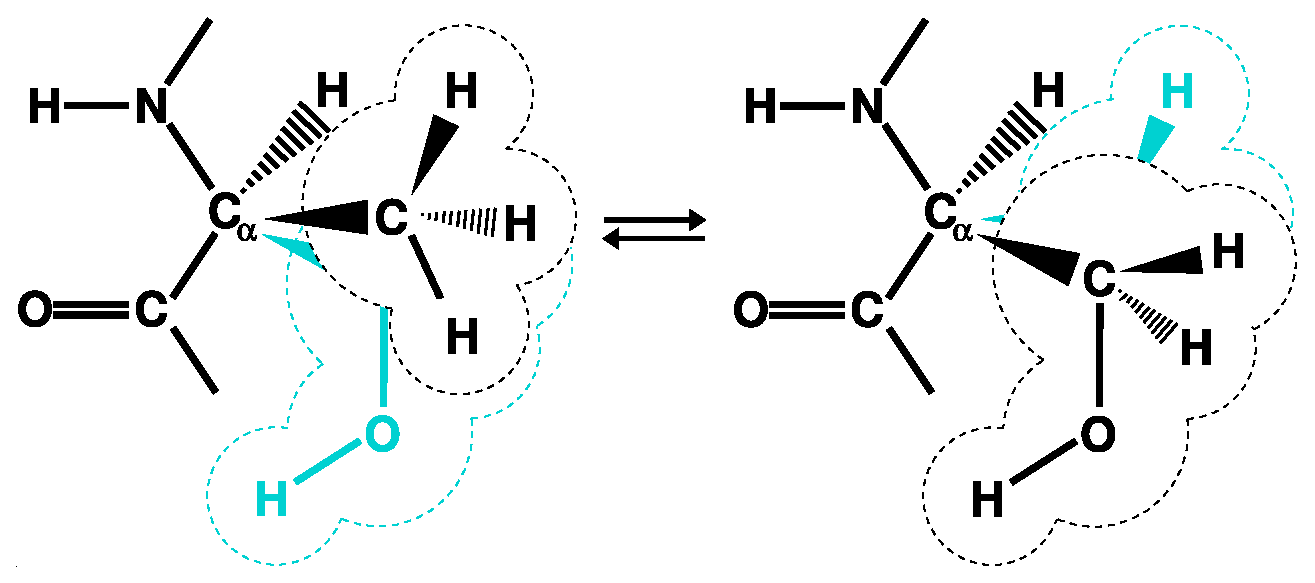
\includegraphics[width=14.5cm]{figures/dual_top}}
  \caption{Dual topology description for an alchemical simulation.
         Case example of the mutation of alanine into glycine.
         The lighter color denotes the non--interacting, alternate
         state.}
  \label{fig:dual_top}
\end{figure}


The energy and forces
are defined as a function of $\lambda$, in such a fashion that 
the interaction of the methyl group of alanine with the rest of 
the protein is effective at the beginning of the simulation,
\ie $\lambda$ = 0, while
the glycine C$_\alpha$ hydrogen does not interact with the rest
of the protein, and {\it vice versa} at the end of the
simulation, \ie $\lambda$ = 1.
For intermediate values of $\lambda$, both the alanine and the glycine
side chains participate in the non--bonded interactions with the rest 
of the protein, scaled on the basis of the current value of $\lambda$.
It should be emphasized that these side chains, however,
do not interact with each other.


It is, therefore, necessary to exclude {\it explicitly} in the setup
those atoms 
that are created from those that will be annihilated in the 
course of the \FEP\ calculation (see ``A tutorial to set up 
alchemical free energy perturbation calculations in \NAMD''
available from the \NAMD\ website).


It is also worth noting that
the free energy calculation does not alter intramolecular
potentials, \ie bond stretch, valence angle deformation, torsions
{\it etc}, during the simulation.
In calculations targetted at the estimation
of free energy differences between two states characterized by
distinct environments --- \eg a ligand bound to a protein in
the first simulation,
and solvated in water, in the second --- as is the 
case for most free energy calculations that make use of a thermodynamic 
cycle, perturbation of intramolecular terms, 
\eg chemical bonds, can be safely
avoided.~\cite{Boresch.99a}



\subsubsection{Implementation of free energy perturbation in \NAMD}


The procedure implemented in \NAMD\ is particularly
adapted for performing free 
energy calculations that split the reaction path into a number of non--physical,
intermediate $\lambda$--states, or ``windows''. Separate simulations 
can be started for each window.
Alternatively, the {\sc Tcl} scripting ability of 
\NAMD\ can be employed advantageously
to perform the complete simulation in a single run.
An example making use of such script is supplied at the end 
of this section.


The following keywords can be used to control free 
energy calculations aimed at alchemical transformations. 

\begin{itemize}

\item
\NAMDCONFWDEF{fep}{ Is alchemical \FEP\ to be performed? }
{{\tt on} or {\tt off}}
{{\tt off}}
{Turns on Hamiltonian scaling and ensemble averaging for alchemical \FEP.}

\item
\NAMDCONF{lambda}{ Coupling parameter value }
{positive decimal between 0.0 and 1.0}
{The coupling parameter value determining the progress of the
perturbation. The non--bonded interactions involving the atoms vanishing
in the course of the MD simulation are scaled by (1-{\tt lambda}), while
those of the growing atoms are scaled by {\tt lambda}.}

\item
\NAMDCONF{lambda2}{Coupling parameter comparison value}
{positive decimal between 0.0 and 1.0}
{The {\tt lambda2} value corresponds to the coupling parameter to be
used for sampling in the next window.  The free energy difference
between {\tt lambda2} and {\tt lambda} is calculated.  Through simulations
at progressive values of {\tt lambda} and {\tt lambda2} the total free
energy difference may be determined.}

\item
\NAMDCONFWDEF{fepEquilSteps}{Number of equilibration steps in the window, 
before data collection}
{positive integer less than {\tt numSteps} or {\tt run}}
{0}
{In each window {\tt fepEquilSteps} steps of equilibration can be
performed before ensemble averaging is initiated. The output also contains
the data gathered during equilibration and is meant for analysis of
convergence properties of the \FEP\ calculation.}

\item
\NAMDCONFWDEF{fepFile}{{\tt pdb} file with perturbation flags}
{filename}
{coordinates}
{{\tt pdb} file to be used for indicating the \FEP\ status for each of
the atoms pertaining to the system. 
If this parameter is not declared specifically, then the
{\tt pdb} file containing the initial coordinates specified by
{\tt coordinates} is utilized for this information.}

\item
\NAMDCONFWDEF{fepCol}{Column in the {\tt fepFile} that carries 
                      the perturbation flag}
{X, Y, Z, O or B}
{B}
{Column of the {\tt pdb} file to use for retrieving the \FEP\ status 
of each atom, \ie a flag that indicates which atom will be perturbed
in the course of the simulation.
A value of {\tt -1} in the specified column indicates the atom will
vanish during the \FEP\ calculation, whereas a value of {\tt 1} 
indicates that the atom will grow.}

\item
\NAMDCONFWDEF{fepOutFreq}{Frequency of \FEP\ energy output in time--steps}
{positive integer}
{5}
{Every {\tt fepOutFreq} number of MD steps, the output file
{\tt fepOutFile} is updated by dumping energies that are
used for ensemble averaging.
This variable could be set to {\tt 1} to include all the 
configurations for ensemble averaging. Yet, it is recommended
to update {\tt fepOutFile}  energies at longer intervals
to avoid large correlation between consecutive configurations.}

\item
\NAMDCONFWDEF{fepOutFile}{\FEP\ energy output filename}
{filename}
{outfilename}
{An output file named {\tt fepOutFile}.fep, generated by \NAMD,
contains the \FEP\ energies, dumped every {\tt fepOutFreq} steps.}

\item
\NAMDCONFWDEF{fepVdWShiftCoeff}{\FEP\ radius-shifting coefficient}
{positive decimal}
{5.}
{This is a radius-shifting coefficient of $\lambda$ that is used 
to construct the modified vdW interactions during alchemical FEP. Providing a positive value for {\tt fepVdWShiftCoeff} ensures that the vdW potential is finite everywhere for small values of $\lambda$, which significantly improves the accuracy and convergence of FEP calculations, and also prevents overlapping particles from making the simulation unstable. During FEP, the inter-atomic distances used in the Lennard-Jones potential are shifted
according to: \\
$r^2 \rightarrow r^2 + {\rm fepVdWShiftCoeff} \times (1. - \lambda)$
}

\item
\NAMDCONFWDEF{fepVdwScaleExp}{\FEP\ Lennerd-Jones parameter scaling exponent}
{decimal}
{0.}
{When constructing the modified vdW interactions during alchemical FEP, the Lennard-Jones parameters are scaled according to:\\
$A \rightarrow A \times \lambda^{2 \times {\rm fepVdwScaleExp}}$ \\
$B \rightarrow B \times \lambda^{\rm fepVdwScaleExp}$
}

%\item
%\NAMDCONFWDEF{fepElecLambdaDelay}{\FEP\ lambda ``delay" for electrostatics}
%{positive decimal}
%{0.}
%{In order to avoid the FEP ``end-point catastrophe", it is often important to make sure that a growing particle does not have an unbounded potential right when it is created (in case that it appears on top of another particle). One way to deal with this for electrostatic interactions, is to allow a bounded scaled vdW potential (using a positive fepVdWShiftCoeff) to first repel all overlapping particles at low values of $\lambda$. As $\lambda$ increases, once the particles are repelled, it is now safe to turn on FEP electrostatics. fepElecLambdaDelay is the value of $\lambda$ at which electrostatic interactins are turned on and start ramping up linearly.}


\end{itemize}


\noindent
{\it Note}: Free energy calculations that rely upon equation~({\ref{master}})
make use of an average temperature, which, in principle, should coincide with
the value of the thermostat. Rather than employing the computed average of $T$,
$\Delta A_{a \rightarrow b}$ is estimated with the target value of the
temperature defined by the user. It is, therefore, necessary to activate
some constant--temperature scheme to carry out \FEP\ calculations. 



\subsubsection{Example of an input file for running \FEP\ alchemical transformations}


The following example illustrates the use of {\sc Tcl} scripting for running
the alchemical \FEP\ feature of \NAMD: 

\begin{verbatim}
fep		on  
fepfile		ion.fep
fepCol		X
fepOutfile	ion.fepout
fepOutFreq	5
fepEquilSteps	5000

set step 0.0
set dstep 0.1

while {$step <= 0.9} {
 lambda $step
 set step [expr $step+$dstep]
 lambda2 $step
 run  10000
}
\end{verbatim}

\noindent
Here, the {\tt pdb} file read by \NAMD\ to extract the information
about perturbed atoms is {\tt biotin.fep}. The pertinent information 
is present in the {\tt X} column. The output file of the free energy
calculation is {\tt biotinr.fepout}, in which energies are written
every {\tt 5} steps.
$\delta \lambda$, the width of the windows, is set to {\tt 0.1}.
{\tt 5000} MD steps are performed in each window to
equilibrate the system. In this particular instance, 
the current value of $\lambda$
is controlled by the statement {\tt set step}. 
The \FEP\ calculation is run until $\lambda$ reaches the
value {\tt 0.9}. In every window, {\tt 10000} MD steps
are performed.


\subsubsection{Description of \FEP\ simulation output }

The {\tt fepOutFile} contains electrostatic and van der Waals energy
data calculated at $\lambda$ and $\lambda2$, written every
{\tt fepOutFreq} steps. The column {\tt dE} is the instantaneous energy
difference for the current configuration. {\tt dE\_avg} and {\tt dG}
are the accumulated energy ensemble average and the corresponding
free energy at the current time step, respectively.
The temperature is specified in the penultimate column. Upon completion
of {\tt fepEquilSteps} steps, the calculation of {\tt dE\_avg} and 
{\tt dG} is restarted. The accumulated net free energy change is output
at each $\lambda$--value and at the end of the simulation. The cumulative
average energy {\tt dE\_avg} value may be summed using, for instance, the 
trapezoidal rule, or a Gaussian quadrature, to obtain an approximate 
TI estimate for the free energy change during the run.





\subsection{Locally Enhanced Sampling}
\label{section:les}

Locally enhanced sampling (LES)~\cite{ROIT91,SIMM98,SIMM00} increases
sampling and transition rates for a portion of a molecule by the use of
multiple non-interacting copies of the enhanced atoms.  These enhanced
atoms experience an interaction (electrostatics, van der Waals, and
covalent) potential that is divided by the number of copies present.
In this way the enhanced atoms can occupy the same space, while the
multiple instances and reduces barriers increase transition rates.

\subsubsection{Structure Generation}

To use LES, the structure and coordinate input files must be modified to
contain multiple copies of the enhanced atoms.  \PSFGEN\ provides the
{\tt multiply} command for this purpose.  \NAMD\ supports a maximum of 15
copies, which should be sufficient.  

Begin by generating the complete molecular structure and guessing
coordinates as described in Sec.~\ref{section:psfgen}.  As the last
operation in your script, prior to writing the psf and pdb files, add
the {\tt multiply} command, specifying the number of copies desired and
listing segments, residues, or atoms to be multiplied.  For example,
\verb#multiply 4 BPTI:56 BPTI:57# will create four copies of the last
two residues of segment BPTI.  You must include all atoms to be
enhanced in a single {\tt multiply} command in order for the bonded
terms in the psf file to be duplicated correctly.  Calling {\tt multiply}
on connected sets of atoms multiple times will produce unpredictable
results, as may running other commands after {\tt multiply}.

The enhanced atoms are duplicated exactly in the structure---they have
the same segment, residue, and atom names.  They are distinguished only
by the value of the B (beta) column in the pdb file, which is 0 for
normal atoms and varies from 1 to the number of copies created for
enhanced atoms.  The enhanced atoms may be easily observed in VMD with
the atom selection \verb#beta != 0#.

\subsubsection{Simulation}

In practice, LES is a simple method used to increase sampling;
no special output is generated.
The following parameters are used to enable LES:

\begin{itemize}

\item
\NAMDCONFWDEF{les}{is locally enhanced sampling active?}{{\tt on} or {\tt
off}}{{\tt off}}
{Specifies whether or not LES is active.}

\item
\NAMDCONF{lesFactor}{number of LES images to use}
{positive integer equal to the number of images present}
{This should be equal to the factor used in {\tt multiply}
 when creating the structure.  The interaction potentials for images is
 divided by {\tt lesFactor}.  
}

\item
\NAMDCONFWDEF{lesFile}{PDB file containing LES flags}{UNIX filename} {{\tt coordinates}}
{PDB file to specify the LES image number of each atom.
If this parameter is not specified, then 
the PDB file containing initial coordinates specified by 
{\tt coordinates} is used.}

\item
\NAMDCONFWDEF{lesCol}{column of PDB file containing LES flags}{{\tt X}, {\tt Y}, {\tt Z}, {\tt O}, or {\tt B}}{{\tt B}}
{Column of the PDB file to specify the LES image number of each atom.
This parameter may specify any of the floating point fields of the PDB file, 
either X, Y, Z, occupancy, or beta-coupling (temperature-coupling).  
A value of 0 in this column indicates that the atom is not enhanced.
Any other value should be a positive integer less than {\tt lesFactor}.}

\end{itemize}

The parameter {\tt lesFactor} may be varied between simulations to
interpolate between full enhancement and normal simulation (although
multiple bonded images are present at all times).  If {\tt lesFactor}
is decreased, the images with flags greater than {\tt lesFactor} will
be decoupled from nonbonded terms, sample based only on bonded terms,
and should therefore be excluded from analysis.  When increasing
{\tt lesFactor} the coordinates of these abandoned images should be
reset to that of another image to avoid any bad initial contacts and
the resulting instability in the simulation.

\subsection{Pair Interaction Calculations}
\label{section:pairinteraction}
\NAMD supportes the calculation of interaction energy calculations between 
two groups of atoms.  When enabled, pair interaction information will be
calculated and printed in the standard output file on its own line at the
same frequency as energy output.  The format of the line is
{\tt PAIR INTERACTION: STEP: {\it step} VDW\_FORCE: {\it fx fy fz} 
ELECT\_FORCE: {\it fx fy fz}}.
The displayed force is the force on atoms in group 1 and is units of 
kcal/mol/\AA. 

For trajectory analysis the 
recommended way to use this set of options is to use the NAMD Tcl scripting 
interface as described in Sec.~\ref{section:tclscripting} to run for
0 steps, so that NAMD prints the energy without performing any dynamics.

\begin{itemize}

\item
\NAMDCONFWDEF{pairInteraction}{is pair interaction calculation active?}
{{\tt on} or {\tt off}}{{\tt off}}
{Specifies whether pair interaction calculation is active.}

\item
\NAMDCONFWDEF{pairInteractionFile}{PDB file containing pair interaction flags}
{UNIX filename}{{\tt coordinates}}
{PDB file to specify atoms to use for pair interaction calculations.  If 
this parameter is not specified, then the PDB file containing initial 
coordinates specified by {\tt coordinates} is used.}

\item
\NAMDCONFWDEF{pairInteractionCol}{column of PDB file containing pair 
interaction flags}{{\tt X}, {\tt Y}, {\tt Z}, {\tt O}, or {\tt B}}{{\tt B}}
{
Column of the PDB file to specify which atoms to use for pair interaction
calculations.  This parameter may specify any of the floating point
fields of the PDB file, either X, Y, Z, occupancy, or beta-coupling
(temperature-coupling).  
}

\item
\NAMDCONFWDEF{pairInteractionSelf}{compute within-group interactions instead of
bewteen groups}{{\tt on} or {\tt off}}{{\tt off}}
{
When active, NAMD will compute bonded and nonbonded interactions only for atoms 
within group 1.  
}
 
\item
\NAMDCONF{pairInteractionGroup1}{Flag to indicate atoms in
group 1?}{integer}{}

\item
\NAMDCONF{pairInteractionGroup2}{Flag to indicate atoms in
group 2?}{integer}{}
{
These options are used to indicate which atoms belong to each interaction 
group.  Atoms with a value in the column specified by {\tt pairInteractionCol} 
equal to {\tt pairInteractionGroup1} will be assigned to group 1; likewise
for group 2.
}

\subsection{Pressure Profile Calculations}
\NAMD\ supports the calculation of lateral pressure profiles as a function of
the z-coordinate in the system.  The algorithm is essentially that described
by Lindahl and Edholm.  The simulation space is partitioned into slabs, and
the virial due to the interaction between two particles is distributed across 
the slabs containing the particles as well as the slabs that lie between the
particles (taking periodic boundary conditions into account).  The diagonal
components of the pressure tensor for each slab are recorded in the 
\NAMD\ output file.  The units of pressure are the same as in the regular 
\NAMD\ pressure output; i.e., bar.

The total virial contains contributions from three components: kinetic energy,
bonded interactions, and nonbonded interactions.  The kinetic and bonded 
components are easily calculated every timestep, and thus may be computed 
during a normal simulation run.  The nonbonded component, however, adds 
significant overhead and has not been implemented for PME calculations.  
The calculation of the nonbonded contribution should be performed offline,
using the saved frames of the trajectory file and a long nonbonded cutoff.

Pressure profile calculations must be performed in a constant volume 
ensemble due to the way the simulation space is partitioned; this constraint
may be relaxed in future versions.  Periodic boundary conditions must also
be enabled.


\item
\NAMDCONFWDEF{pressureProfileOn}{compute pressure profile}{{\tt on} or {\tt off}}{{\tt off}}
{
When active, NAMD will compute kinetic and bonded contributions to the 
pressure profile.  Results will be recorded in the \NAMD\ output file
in lines with the format
{\tt PRESSUREPROFILE: ts Axx Ayy Azz Bxx Byy Bzz ... }, where {\tt ts} is the
timestep, followed by the three diagonal components of the pressure tensor 
in the first
slab (the slab with lowest {\it z}), then the next lowest slab, and so forth.
NAMD will also output the pressure profile averaged over all the steps since
the last output.  The format of this line is 
{\tt PRESSUREPROFILEAVG: ts Axx Ayy Azz ... }; i.e., exactly as for the
instantaneous pressure.  It is recommended to use the averaged pressure profile
instead of the instantaneous value as this will give better statistics and
may prevent artifacts when using multiple timestepping.
}
\item
\NAMDCONFWDEF{pressureProfileSlabs}{Number of slabs in the spatial partition}{Positive integer}{10}{
\NAMD\ divides the entire periodic cell into horizontal slabs of equal 
thickness; {\tt pressureProfileSlabs} specifies the number of such slabs.
}

\item
\NAMDCONFWDEF{pressureProfileFreq}{How often to output pressure profile
data}{Positive integer}{1}{
Specifies the number of timesteps between output of pressure profile data.
}

\item
\NAMDCONFWDEF{pressureProfileNonbonded}{Compute nonbonded pressure profile
contribution}{{\tt on} or {\tt off}}{{\tt off}}{
When enabled, only the nonbonded contribution to the pressure profile will be
computed.  For trajectory analysis the 
recommended way to use this option is to use the \NAMD\ Tcl scripting 
interface as described in Sec.~\ref{section:tclscripting} to run for
0 steps, so that NAMD prints the pressure profile without performing any 
dynamics.
}
\end{itemize}

Here is an example snippet from a \NAMD\ input that can be used to compute
the nonbonded component of the pressure profile.  It assumes that the 
coordinates were saved in three dcd files ({\tt pp01.dcd}, {\tt pp02.dcd},
and {\tt pp03.dcd}) every 500 timesteps.  The {\tt pressureProfileSlabs}
must be the same as was used for the calculation of the bonded part of
the pressure.
\begin{verbatim}
cutoff		     18.0
switching	     on
switchdist	   16.5	
pairlistdist	 18.5 

pressureProfile	on
pressureProfileSlabs 60 
pressureProfileFreq 100 
pressureProfileNonbonded on

# Assume that coordinates were written to the dcd files every 500 timesteps.
set ts 500
foreach dcd { pp01.dcd pp02.dcd pp03.dcd } {
  coorfile open dcd $dcd
  while { [coorfile read] != -1 } {
    firstTimestep $ts 
    run 0 
    incr ts 500
  }
  coorfile close
}
\end{verbatim}



% Equivalence with X-PLOR parameters
\newpage
\section{Translation between \NAMD\ and X-PLOR configuration parameters}
\label{section:xplorequiv}

\NAMD\ was designed to provide many of the same molecular dynamics functions that
X-PLOR provides.  As such, there are many similarities between the types of parameters
that must be passed to both X-PLOR and \NAMD.  This section describes relations
between similar \NAMD\ and X-PLOR parameters.  

\begin{itemize}

\item
\XNCOMP{cutoff, eleccutoff, vdwcutoff}{CTOFNB}
{When full electrostatics are not in use within \NAMD, 
these parameters have exactly the same meaning 
--- the distance at which electrostatic 
and van der Waals forces are truncated.  
When full electrostatics are in use
within \NAMD, the meaning is still very similar.  
The van der Waals force is still truncated at the specified distance, 
and the electrostatic force is still computed at every timestep 
for interactions within the specified distance.  
However, the \NAMD\ integration uses multiple time stepping to 
compute electrostatic force interactions beyond this distance 
every {\tt stepspercycle} timesteps.}

\item
\XNCOMP{vdwswitchdist}{CTONNB}
{Distance at which the van der Waals switching function becomes active.}

\item 
\XNCOMP{pairlistdist}{CUTNb}
{Distance within which interaction pairs will be included in pairlist.}

\item
\XNCOMP{1-4scaling}{E14Fac}{Scaling factor for 1-4 pair electrostatic interactions.}

\item
\XNCOMP{dielectric}{EPS}{Dielectric constant.}

\item
\XNCOMP{exclude}{NBXMod}
{Both parameters specify which atom pairs 
to exclude from non-bonded interactions.  
The ability to ignore explicit exclusions is {\it not} present within \NAMD, 
thus only positive values of {\tt NBXMod} have \NAMD\ equivalents.  
These equivalences are
\begin{itemize}
\item
{\tt NBXMod=1} is equivalent to {\tt exclude=none} 
--- no atom pairs excluded, 
\item
{\tt NBXMod=2} is equivalent to {\tt exclude=1-2} 
--- only 1-2 pairs excluded, 
\item
{\tt NBXMod=3} is equivalent to {\tt exclude=1-3} 
--- 1-2 and 1-3 pairs excluded, 
\item
{\tt NBXMod=4} is equivalent to {\tt exclude=1-4} 
--- 1-2, 1-3, and 1-4 pairs excluded, 
\item
{\tt NBXMod}=5 is equivalent to {\tt exclude=scaled1-4} 
--- 1-2 and 1-3 pairs excluded, 1-4 pairs modified. 
\end{itemize}}

\item
\XNCOMP{switching}{SHIFt, VSWItch, and TRUNcation}
{Activating the \NAMD\ option {\tt switching} is equivalent 
to using the X-PLOR options {\tt SHIFt} and {\tt VSWItch}.  
Deactivating {\tt switching} is equivalent 
to using the X-PLOR option {\tt TRUNcation}.}

\item
\XNCOMP{temperature}{FIRSttemp}
{Initial temperature for the system.}

\item
\XNCOMP{rescaleFreq}{IEQFrq}
{Number of timesteps between velocity rescaling.}

\item
\XNCOMP{rescaleTemp}{FINAltemp}
{Temperature to which velocities are rescaled.}

\item
\XNCOMP{restartname}{SAVE}{Filename prefix for the restart files.}

\item
\XNCOMP{restartfreq}{ISVFrq}
{Number of timesteps between the generation of restart files.}

\item
\XNCOMP{DCDfile}{TRAJectory}
{Filename for the position trajectory file.} 

\item
\XNCOMP{DCDfreq}{NSAVC}
{Number of timesteps between writing coordinates to the trajectory file.}

\item
\XNCOMP{velDCDfile}{VELOcity}
{Filename for the velocity trajectory file.}

\item
\XNCOMP{velDCDfreq}{NSAVV}
{Number of timesteps between writing velocities to the trajectory file.} 

\item
\XNCOMP{numsteps}{NSTEp}
{Number of simulation timesteps to perform.}

\end{itemize}



% Sample configuration files
\newpage
\section{Sample configuration files}
\label{section:sample}
This section contains some simple example \NAMD\ configuration files to serve
as templates.
\prettypar
This file shows a simple configuration file for alanin.  
It performs basic dynamics
with no output files or special features.

\begin{verbatim}

timestep        0.5
numsteps        10000

cwd             /scratch              #  Specify a working directory 

structure       alanin.psf
parameters      alanin.params
coordinates     alanin.pdb

exclude         scaled1-4
1-4scaling      0.4
outputname      output
margin          1.0
stepspercycle   10
temperature     300.0

switching       on
switchdist      7.0
cutoff          8.0
pairlistdist    9.0

\end{verbatim}

\newpage
This file is again for alanin, 
but shows a slightly more complicated configuration.  
A coordinate trajectory file and a set of restart files 
are produced every ten timesteps.  
Langevin dynamics are also active in this configuration.  

\begin{verbatim}
timestep        0.5

numsteps        10000

structure       alanin.psf
parameters      alanin.params
coordinates     alanin.pdb
exclude         scaled1-4
1-4scaling      0.4
outputname      output
margin          1.0
stepspercycle   10
temperature     300.0

switching       on
switchdist      7.0
cutoff          8.0
pairlistdist    9.0

DCDfile         alanin.dcd
DCDfreq         10

restartname     alanin.restart
restartfreq     10

langevin        on
langevinTemp    300.0
langevinCol     O
\end{verbatim}

\newpage
This file shows another simple configuration file for alanin, 
but this time with full electrostatics using DPMTA.  

\begin{verbatim}

timestep        0.5
numsteps        10000

cwd             /scratch        #  Specify a working directory 

structure       alanin.psf
parameters      alanin.params
coordinates     alanin.pdb

exclude         scaled1-4
1-4scaling      0.4
outputname      output
margin          1.0
stepspercycle   10
temperature     300.0

switching       on
switchdist      7.0
cutoff          8.0
pairlistdist    9.0

# DPMTA parameters
FMA             on
FMAMp           8
FMALevels       3
FMAFFT          on
FMAFFTBlock     4

\end{verbatim}
\newpage


% Description of how to run namd
\newpage
%%%%%%%%%%%%%%%%%%%%%%%%%%%%%%%%%%%%%%%%%%%%%%%%%%%%%%%%%%%%%%%%%%%%%%%%%%%%
%                                                                          %
%              (C) Copyright 1995 The Board of Trustees of the             %
%                          University of Illinois                          %
%                           All Rights Reserved                            %
%								  	   %
%%%%%%%%%%%%%%%%%%%%%%%%%%%%%%%%%%%%%%%%%%%%%%%%%%%%%%%%%%%%%%%%%%%%%%%%%%%%

\section{Running \NAMD}
\label{section:run}

NAMD runs on a variety of serial and parallel platforms.  While it is
trivial to launch a serial program, a parallel program depends on a
platform-specific library such as MPI to launch copies of itself on
other nodes and to provide access to a high performance network such
as Myrinet or InfiniBand if one is available.

For typical workstations (Windows, Linux, Mac OS X, or other Unix)
with only ethernet networking (hopefully gigabit), NAMD uses the
Charm++ native communications layer and the program charmrun to launch
namd2 processes for parallel runs (either exclusively on the local
machine with the ++local option or on other hosts as specified by a
nodelist file).  The namd2 binaries for these platforms can also be
run directly (known as standalone mode) for single process runs.

\subsection{Individual Windows, Linux, Mac OS X, or Other Unix Workstations}

Individual workstations use the same version of NAMD as workstation
networks, but running NAMD is much easier.  If your machine has only
one processor core you can run the any non-MPI namd2 binary directly:

\begin{verbatim}
  namd2 <configfile>
\end{verbatim}

For multicore workstations, Windows and Mac OX X (Intel) released binaries
are based on ``multicore'' builds of Charm++ that can run multiple threads.
These multicore builds lack a network layer, so they can only be used on a
single machine.
The Solaris (Sparc and x86-64) released binaries are based on ``smp''
builds of Charm++ that can be used with multiple threads on either a
single machine like a multicore build, or across a network.
For best performance use one thread per processor with the +p option:

\begin{verbatim}
  namd2 +p<procs> <configfile>
\end{verbatim}

For other multiprocessor workstations the included charmrun program is
needed to run multiple namd2 processes.  The ++local option is also
required to specify that only the local machine is being used:

\begin{verbatim}
  charmrun namd2 ++local +p<procs> <configfile>
\end{verbatim}

You may need to specify the full path to the namd2 binary.

\subsection{Linux Clusters with InfiniBand Or Other High-Performance Networks}

Charm++ provides a special ibverbs network layer that uses InfiniBand
networks directly through the OpenFabrics OFED ibverbs library.  This
avoids efficiency and portability issues associated with MPI.  Look for
pre-built ibverbs NAMD binaries or specify ibverbs when building Charm++.

Writing batch job scripts to run charmrun in a queueing system can be
challenging.  Since most clusters provide directions for using mpiexec
to launch MPI jobs, charmrun provides a ++mpiexec option to use mpiexec
to launch non-MPI binaries.  If "mpiexec -np {\em procs} ..." is not
sufficient to launch jobs on your cluster you will need to write an
executable mympiexec script like the following from TACC:

\begin{verbatim}
  #!/bin/csh
  shift; shift; exec ibrun $*
\end{verbatim}

The job is then launched (with full paths where needed) as:

\begin{verbatim}
  charmrun +p<procs> ++mpiexec ++remote-shell mympiexec namd2 <configfile>
\end{verbatim}

For workstation clusters and other massively parallel machines with
special high-performance networking, NAMD uses the system-provided MPI
library (with a few exceptions) and standard system tools such as mpirun
are used to launch jobs.  Since MPI libraries are very often incompatible
between versions, you will likely need to recompile NAMD and its
underlying Charm++ libraries to use these machines in parallel (the
provided non-MPI binaries should still work for serial runs.) The provided
charmrun program for these platforms is only a script that attempts to
translate charmrun options into mpirun options, but due to the diversity
of MPI libraries it often fails to work.

\subsection{Linux or Other Unix Workstation Networks}

The same binaries used for individual workstations as described above
(other than pure ``multicore'' builds and MPI builds)
can be used with charmrun to run in parallel on a workstation network.
The only difference is that you must provide a ``nodelist'' file listing
the machines where namd2 processes should run, for example:

\begin{verbatim}
  group main
  host brutus
  host romeo
\end{verbatim}

The ``group main'' line defines the default machine list.  Hosts brutus
and romeo are the two machines on which to run the simulation.  Note
that charmrun may run on one of those machines, or charmrun may run
on a third machine.  All machines used for a simulation must be of the
same type and have access to the same namd2 binary.

By default, the ``rsh'' command is used to start namd2
on each node specified in the nodelist file.  You can change this via
the CONV\_RSH environment variable, i.e., to use ssh instead of rsh run
``setenv CONV\_RSH ssh'' or add it to your login or batch script.  You
must be able to connect to each node via rsh/ssh without typing your
password; this can be accomplished via a .rhosts files in your home
directory, by an /etc/hosts.equiv file installed by your sysadmin, or
by a .ssh/authorized\_keys file in your home directory.  You should
confirm that you can run ``ssh hostname pwd'' (or ``rsh hostname pwd'')
without typing a password before running NAMD.  Contact your local
sysadmin if you have difficulty setting this up.  If you are unable to
use rsh or ssh, then add ``setenv CONV\_DAEMON'' to your script and run 
charmd (or charmd\_faceless, which produces a log file) on every node.

You should now be able to try running NAMD as:

\begin{verbatim}
  charmrun namd2 +p<procs> <configfile>
\end{verbatim}

If this fails or just hangs, try adding the ++verbose option to see
more details of the startup process.  You may need to specify the full
path to the namd2 binary.  Charmrun will start the number of processes
specified by the +p option, cycling through the hosts in the nodelist
file as many times as necessary.  You may list multiprocessor machines
multiple times in the nodelist file, once for each processor.

You may specify the nodelist file with the ``++nodelist'' option and the
group (which defaults to ``main'') with the ``++nodegroup'' option.  If
you do not use ``++nodelist'' charmrun will first look for ``nodelist''
in your current directory and then ``.nodelist'' in your home directory.

Some automounters use a temporary mount directory which is prepended
to the path returned by the pwd command.  To run on multiple machines
you must add a ``++pathfix'' option to your nodelist file.  For example:

\begin{verbatim}
  group main ++pathfix /tmp\_mnt /
  host alpha1
  host alpha2
\end{verbatim}

There are many other options to charmrun and for the nodelist file.
These are documented at in the Charm++ Installation and Usage Manual
available at http://charm.cs.uiuc.edu/manuals/ and a list of available
charmrun options is available by running charmrun without arguments.

If your workstation cluster is controlled by a queueing system you
will need build a nodelist file in your job script.  For example, if
your queueing system provides a HOST\_FILE environment variable:

\begin{verbatim}
  set NODES = `cat $HOST_FILE`
  set NODELIST = $TMPDIR/namd2.nodelist
  echo group main >! $NODELIST
  foreach node ( $nodes )
    echo host $node >> $NODELIST
  end
  @ NUMPROCS = 2 * $#NODES
  charmrun namd2 +p$NUMPROCS ++nodelist $NODELIST <configfile>
\end{verbatim}

Note that NUMPROCS is twice the number of nodes in this example.
This is the case for dual-processor machines.  For single-processor
machines you would not multiply \$\#NODES by two.

Note that these example scripts and the setenv command are for the csh
or tcsh shells.  They must be translated to work with sh or bash.

\subsection{Windows Workstation Networks}

These are no longer supported, but NAMD has been reported to compile
on Windows HPC Server.

\subsection{SGI Altix}

Be sure that the {\tt MPI\_DSM\_DISTRIBUTE} environment variable is set, then
use the Linux-Itanium-MPI-Altix version of NAMD along with the system mpirun:

\begin{verbatim}
mpirun -np <procs> <configfile>
\end{verbatim}

\subsection{IBM POWER Clusters}

Run the MPI version of NAMD as you would any POE program.  The options
and environment variables for poe are various and arcane, so you should
consult your local documentation for recommended settings.  As an
example, to run on Blue Horizon one would specify:

\begin{verbatim}
  poe namd2 <configfile> -nodes <procs/8> -tasks_per_node 8
\end{verbatim}

\subsection{CUDA GPU Acceleration}

NAMD only uses the GPU for nonbonded force evaluation.  Energy evaluation
is done on the CPU.  To benefit from GPU acceleration you should set
outputEnergies to 100 or higher in the simulation config file.  Some
features are unavailable in CUDA builds, including alchemical free
energy perturbation.

As this is a new feature you are encouraged to test all simulations
before beginning production runs.  Forces evaluated on the GPU differ
slightly from a CPU-only calculation, an effect more visible in reported
scalar pressure values than in energies.

To benefit from GPU acceleration you will need a CUDA build of NAMD
and a recent high-end NVIDIA video card.  CUDA builds will not function
without a CUDA-capable GPU.  You will also need to be running the
NVIDIA Linux driver version 195.17 or newer (NAMD 2.7b4 released binaries
are built with CUDA 2.3, but can be built with 3.0 or 3.1 as well).

Finally, the libcudart.so.2 included with the binary (the one copied from
the version of CUDA it was built with) must be in a directory in your
LD\_LIBRARY\_PATH before any other libcudart.so libraries.  For example:

\begin{verbatim}
  setenv LD_LIBRARY_PATH ".:$LD_LIBRARY_PATH"
  (or LD_LIBRARY_PATH=".:$LD_LIBRARY_PATH"; export LD_LIBRARY_PATH)
  ./namd2 +idlepoll <configfile>
  ./charmrun ++local +p4 ./namd2 +idlepoll <configfile>
\end{verbatim}

When running CUDA NAMD always add +idlepoll to the command line.  This
is needed to poll the GPU for results rather than sleeping while idle.

Each namd2 process can use only one GPU.  Therefore you will need to run
at least one process for each GPU you want to use.  Multiple processes
can share a single GPU, usually with an increase in performance.  NAMD
will automatically distribute processes equally among the GPUs on a node.
Specific GPU device IDs can be requested via the +devices argument on
the namd2 command line, for example:

\begin{verbatim}
  ./charmrun ++local +p4 ./namd2 +idlepoll +devices 0,2 <configfile>
\end{verbatim}

Devices are selected cyclically from those available, so in the above
example processes 0 and 2 will share device 0 and processes 1 and 3 will
share device 2.  One could also specify +devices 0,0,2,2 to cause device
0 to be shared by processes 0 and 1, etc.  GPUs with two or fewer
multiprocessors are ignored unless specifically requested with +devices.

While charmrun with ++local will preserve LD\_LIBRARY\_PATH, normal
charmrun does not.  You can use charmrun ++runscript to add the namd2
directory to LD\_LIBRARY\_PATH with the following executable runscript:

\begin{verbatim}
  #!/bin/csh
  setenv LD_LIBRARY_PATH "${1:h}:$LD_LIBRARY_PATH"
  $*
\end{verbatim}

For example:

\begin{verbatim}
  ./charmrun ++runscript ./runscript +p8 ./namd2 +idlepoll <configfile>
\end{verbatim}

An InfiniBand network is highly recommended when running CUDA-accelerated
NAMD across multiple nodes.  You will need either an ibverbs NAMD binary
(available for download) or an MPI NAMD binary (must build Charm++ and
NAMD as described above) to make use of the InfiniBand network.

The CUDA (NVIDIA's graphics processor programming platform) code in
NAMD is completely self-contained and does not use any of the CUDA
support features in Charm++.  When building NAMD with CUDA support
you should use the same Charm++ you would use for a non-CUDA build.
Do NOT add the cuda option to the Charm++ build command line.  The
only changes to the build process needed are to add --with-cuda and
possibly --cuda-prefix ... to the NAMD config command line.

\subsection{Memory Usage}

NAMD has traditionally used less than 100MB of memory even for systems
of 100,000 atoms.  With the reintroduction of pairlists in NAMD 2.5,
however, memory usage for a 100,000 atom system with a 12A cutoff can
approach 300MB, and will grow with the cube of the cutoff.  This extra
memory is distributed across processors during a parallel run, but a
single workstation may run out of physical memory with a large system.

To avoid this, NAMD now provides a pairlistMinProcs config file option
that specifies the minimum number of processors that a run must use
before pairlists will be enabled (on fewer processors small local
pairlists are generated and recycled rather than being saved, the
default is ``pairlistMinProcs 1'').  This is a per-simulation rather than
a compile time option because memory usage is molecule-dependent.

Additional information on reducing memory usage may be found at
http://www.ks.uiuc.edu/Research/namd/wiki/index.cgi?NamdMemoryReduction

\subsection{Improving Parallel Scaling}

While NAMD is designed to be a scalable program, particularly for
simulations of 100,000 atoms or more, at some point adding additional
processors to a simulation will provide little or no extra performance.
If you are lucky enough to have access to a parallel machine you should
measure NAMD's parallel speedup for a variety of processor counts when
running your particular simulation.  The easiest and most accurate way
to do this is to look at the ``Benchmark time:'' lines that are printed
after 20 and 25 cycles (usually less than 500 steps).  You can monitor
performance during the entire simulation by adding ``outputTiming {\em steps}''
to your configuration file, but be careful to look at the ``wall time''
rather than ``CPU time'' fields on the ``TIMING:'' output lines produced.
For an external measure of performance, you should run simulations of
both 25 and 50 cycles (see the stepspercycle parameter) and base your
estimate on the additional time needed for the longer simulation in
order to exclude startup costs and allow for initial load balancing.

We provide both standard (UDP) and TCP based precompiled binaries
for Linux clusters.  We have observed that the TCP version is better
on our dual processor clusters with gigabit ethernet while the basic
UDP version is superior on our single processor fast ethernet cluster.
When using the UDP version with gigabit you can add the +giga option
to adjust several tuning parameters.  Additional performance may be
gained by building NAMD against an SMP version of Charm++ such as
net-linux-smp or net-linux-smp-icc.  This will use a communication
thread for each process to respond to network activity more rapidly.
For dual processor clusters we have found it that running two separate
processes per node, each with its own communication thread, is faster
than using the charmrun ++ppn option to run multiple worker threads.
However, we have observed that when running on a single hyperthreaded
processor (i.e., a newer Pentium 4) there is an additional 15\% boost
from running standalone with two threads (namd2 +p2) beyond running
two processors (charmrun namd2 ++local +p2).  For a cluster of single
processor hyperthreaded machines an SMP version should provide very
good scaling running one process per node since the communication
thread can run very efficiently on the second virtual processor.  We
are unable to ship an SMP build for Linux due to portability problems
with the Linux pthreads implementation needed by Charm++.

Extremely short cycle lengths (less than 10 steps) will also limit
parallel scaling, since the atom migration at the end of each cycle
sends many more messages than a normal force evaluation.  Increasing
pairlistdist from, e.g., cutoff + 1.5 to cutoff + 2.5, while also
doubling stepspercycle from 10 to 20, may increase parallel scaling,
but it is important to measure.  When increasing stepspercycle, also
try increasing pairlistspercycle by the same proportion.

NAMD should scale very well when the number of patches (multiply the
dimensions of the patch grid) is larger or rougly the same as the
number of processors.  If this is not the case, it may be possible
to improve scaling by adding ``twoAwayX yes'' to the config file,
which roughly doubles the number of patches.  (Similar options
twoAwayY and twoAwayZ also exist, and may be used in combination,
but this greatly increases the number of compute objects.  twoAwayX
has the unique advantage of also improving the scalability of PME.)
\index{twoAwayX} \index{twoAwayY} \index{twoAwayZ}

Additional performance tuning suggestions and options are described
at http://www.ks.uiuc.edu/Research/namd/wiki/?NamdPerformanceTuning



% How to get and install namd
\newpage
%%%%%%%%%%%%%%%%%%%%%%%%%%%%%%%%%%%%%%%%%%%%%%%%%%%%%%%%%%%%%%%%%%%%%%%%%%%%
%                                                                          %
%              (C) Copyright 1995 The Board of Trustees of the             %
%                          University of Illinois                          %
%                           All Rights Reserved                            %
%								  	   %
%%%%%%%%%%%%%%%%%%%%%%%%%%%%%%%%%%%%%%%%%%%%%%%%%%%%%%%%%%%%%%%%%%%%%%%%%%%%

%%%%%%%%%%%%%%%%%%%%%%%%%%%%%%%%%%%%%%%%%%%%%%%%%%%%%%%%%%%%%%%%%%%%%%%%%%%%
% RCS INFORMATION:
%
%       $RCSfile: ug_avail.tex,v $
%       $Author: dhardy $        $Locker:  $                $State: Exp $
%       $Revision: 1.1 $      $Date: 1998/01/05 21:12:31 $
%
%%%%%%%%%%%%%%%%%%%%%%%%%%%%%%%%%%%%%%%%%%%%%%%%%%%%%%%%%%%%%%%%%%%%%%%%%%%%
% DESCRIPTION:
%	This section is part of the NAMD Users Guide and describes the
% the availability and installation of NAMD
%
%%%%%%%%%%%%%%%%%%%%%%%%%%%%%%%%%%%%%%%%%%%%%%%%%%%%%%%%%%%%%%%%%%%%%%%%%%%%
% REVISION HISTORY:
%
% $Log: ug_avail.tex,v $
% Revision 1.1  1998/01/05 21:12:31  dhardy
% user guide, first draft
%
% Revision 1.13  1997/08/07 17:28:20  dhardy
% minor revisions
%
% Revision 1.12  1997/08/07 15:54:32  dhardy
% edit presentation style, add control of precision during compile
%
% Revision 1.11  1997/02/25 22:35:20  dalke
% *** empty log message ***
%
% Revision 1.10  1996/06/06  18:02:01  dalke
% fixed typos for 1.4 release
%
% Revision 1.9  1996/05/15  19:21:07  jean
% ready (I hope) for 1.4 beta release
%
% Revision 1.8  1996/03/10 20:35:16  jean
% namd -> \NAMD\
%
% Revision 1.7  1996/03/10 20:11:27  jean
% minor polishing
%
% Revision 1.6  1995/10/04 14:41:39  nelson
% Fixed spelling and changed status of IBM SP1 and SP2
%
% Revision 1.5  95/06/30  15:56:19  15:56:19  gursoy (Attila Gursoy)
% added Power Challenge and SP2
% 
% Revision 1.4  95/06/30  15:49:44  15:49:44  gursoy (Attila Gursoy)
% *** empty log message ***
% 
% Revision 1.3  95/06/30  15:37:43  15:37:43  gursoy (Attila Gursoy)
% added platforms
% 
% Revision 1.2  95/06/28  23:55:46  23:55:46  gursoy (Attila Gursoy)
% first draft
% 
% Revision 1.1  95/06/19  16:08:15  16:08:15  nelson (Mark T. Nelson)
% Initial revision
% 
%%%%%%%%%%%%%%%%%%%%%%%%%%%%%%%%%%%%%%%%%%%%%%%%%%%%%%%%%%%%%%%%%%%%%%%%%%%%

\section{\NAMD\ Availability and Installation}

\NAMD\ is distributed freely for non-profit use.  Portability 
across various architectures is achieved by using widely available 
message-passing software layers.  \NAMD\ currently runs on 
PVM, a message-passing library available for distributed and 
parallel computers.  
%%  Charm is an object-based parallel programming environment
%% available from University of Illinois (\verb+http://charm.cs.uiuc.edu+).
%% Currently, at the ftp site, only the PVM version of \NAMD\ is available.
\prettypar
This section describes how to obtain \NAMD\ and how to install the PVM based 
version.  In order to compile and run this version, PVM 3.x must be 
installed on the target machines.  

\subsection{How to obtain \NAMD}

\NAMD\ is available as the compressed tar file 
{\tt namd-xxx.tar.gz} obtained via anonymous 
FTP from the server {\tt ftp.ks.uiuc.edu} in the directory 
{\tt pub/mdscope/namd}.  
Directories from this release and their content are as follows: 
\begin{tabbing}
xxxxx \= xxxxxxxx\= \kill \\
\> {\tt DPMTA} \>
         DPMTA for HPUX-9.x from the Scientific Computing group at Duke \\
\> {\tt doc} \> 
         Documentation for \NAMD\ \\
\> {\tt mdcomm} \> 
         MDComm software, currently available only for HPUX-9.x and 
IRIX-5.x \\ 
\> {\tt src} \>
         \NAMD\ source code \\
\> {\tt sample} \>
         Sample \NAMD\ configuration file and protein
\end{tabbing}

DPMTA is the Distributed Parallel Multipole Treecode Algorithm 
developed by the scientific computing group at Duke University.  
\NAMD\ is capable of interacting with DPMTA to provide full electrostatic 
calculations.  A pre-compiled version of DPMTA for HP systems is included 
with this release for convenience.  The source code, 
which can be compiled for other platforms, 
may be obtained directly from Duke via anonymous FTP from 
the server {\tt ftp.ee.duke.edu} in the directory {\tt /pub/SciComp/src}.
\prettypar
MDComm is a library and set of daemon processes that allow \NAMD\ to 
communicate with the graphics program \VMD\ running on a remote machine 
via TCP/IP.  This library is currently available only for HPUX-9.x and 
IRIX-5.x systems.  
\prettypar
MTS is the Memory Tuning Software from New Code, Inc\. which provides a 
faster memory allocation scheme than that available from most UNIX 
implementations.  On HPUX-9.x systems, it achieves an increase in overall 
\NAMD\ performance of about 10\%.  This software is available from
NewCode, Inc.
\prettypar
If any of 
DPMTA, MDComm, or MTS are not available or desired, simply comment 
out the corresponding 
section of the appropriate \verb+Makedata.<architecture>+ file.  

\subsection{Platforms on which \NAMD\ will currently run}
\NAMD\ is expected to run on any parallel platform with a C++ compiler
and PVM version 3.3.6 or later.
Some minor tuning of system parameters or compiler flags 
may be required.  Such parameters include PVM buffer sizes, etc.  
\NAMD\ has been compiled and tested on the following platforms:  
\begin{itemize}
\item HP workstations (HPUX)
\item SGI workstations  (IRIX5)
\item IBM workstations (AIX)
\item Cray T3D
\item Convex Exemplar
\item IBM SP1 and SP2 using PVMe
\end{itemize}
%% List of machines that we plan to test soon include the SGI Power
%% Challenge and Intel Paragon.

\subsection{Compiling \NAMD}
To compile \NAMD\ for a particular machine, follow these steps:  
%%  \begin{tabbing}
%%  xxxxx \= xxxxx \= \kill \\
%%  \> 1. \> Go to the {\tt src} directory. \\
%%  \> 2. \> Edit {\tt Makefile} and change the ARCH variable to the desired 
%%           system\\ 
%%  \>    \> \eg, one of HPUX9, IRIX5, AIX, T3D, or Exemplar. \\
%%  \> 3. \> Edit the \verb+Makedata.<architecture>+ file to get the 
%%           correct options\\
%%  \>    \>  and directory specifications for your platform.  \\
%%  \> 4. \> Type \verb!make!.
%%  \end{tabbing}
\begin{enumerate}
\item 
Go to the {\tt src} directory. 
\item
Edit {\tt Makefile} and change the ARCH variable to the desired system 
\eg, one of HPUX9, IRIX5, AIX, T3D, or Exemplar.  
\item 
Edit the \verb+Makedata.<architecture>+ file to get the 
correct options and directory specifications for your platform.  
For example, precision can be controlled at compile time 
to yield single rather than the default double precision.  
The \verb!ARCH_COPTS! (C compiler options) variable 
would need to be changed 
in \verb+Makedata.<architecture>+ 
to define \verb!SHORTREALS! to the preprocessor.  
\item
Type \verb!make!.
\end{enumerate}
Pre-compiled binaries are provided for HP and SGI workstations.

\subsection{Documentation}
The directory {\tt doc} contains three documents:
\begin{itemize}
\item the \UG\ ({\tt ug.ps}, this document) describes how to use \NAMD, 
\item the \PG\ ({\tt pg.ps}) provides a complete description of \NAMD\ and 
  its implementation, 
\item {\tt configsheet.ps} provides a one page summary of the 
  configuration options for \NAMD.  
\end{itemize}



\newpage
\bibliographystyle{abbrv}
%\bibliography{group,tbpub,ug}
\bibliography{ug}

% that's all, folks
\end{document}

